\documentclass[a4paper,12pt]{memoir}

\usepackage{hyperref}
\usepackage[margin=2.5cm,left=3.5cm]{geometry}
\usepackage[backend=biber,style=apa]{biblatex}
\usepackage[french,english]{babel}
\usepackage{amsmath}
\usepackage{amsfonts}
\usepackage{amsthm}
\usepackage{amssymb}
\usepackage{graphicx} % includegraphics
\usepackage{url} % url
\usepackage{tikz} % tikz images
\usepackage{bm} % bold font math
\usepackage{soul} % ???
\usepackage{tabularx} % Equal-size column tables
\usepackage{booktabs} % nice tables
\usepackage{algorithm}
\usepackage{algpseudocode}
\usepackage{enumerate} % improvement over lists
\usepackage{pifont} % ticks and cross characters
\usepackage{subcaption} % sub-figures
\usepackage{draftwatermark} % well, a draft watermark

\SetWatermarkLightness{0.9} % Greyness of the watermark

\definecolor{themeblue}{RGB}{20, 116, 230}
\definecolor{darkerblue}{RGB}{5, 71, 149}
\definecolor{lightblue}{RGB}{103,163,235}

\definecolor{themeyellow}{RGB}{255, 241, 1}
\definecolor{darkeryellow}{RGB}{228, 215, 0}
\definecolor{lightyellow}{RGB}{255,246,99}

\definecolor{themeorange}{RGB}{255, 156, 1}
\definecolor{darkerorange}{RGB}{228, 140, 0}
\definecolor{lightorange}{RGB}{255,195,99}

\definecolor{themepurple}{RGB}{126, 18, 231}
\definecolor{darkerpurple}{RGB}{81, 5, 154}
\definecolor{lightpurple}{RGB}{170,102,236}


\theoremstyle{definition}
\newtheorem{definition}{Definition}

\newcommand{\TP}{\textit{TP}}
\newcommand{\FP}{\textit{FP}}
\newcommand{\TN}{\textit{TN}}
\newcommand{\FN}{\textit{FN}}
\newcommand{\Fmeasure}{\textit{F1}}
\newcommand{\precision}{\textit{precision}}
\newcommand{\recall}{\textit{recall}}
\newcommand{\TPR}{\textit{TPR}}
\newcommand{\FPR}{\textit{FPR}}
\newcommand{\lift}{\textit{lift}}
\newcommand{\AUC}{\textit{AUC}}
\newcommand{\MB}{\textbf{MB}}
\DeclareMathOperator*{\argmax}{arg\,max}

\newcolumntype{Y}{>{\centering\arraybackslash}X} % Centered, equal-width table column

\newcommand{\ok}{\textcolor{green}{\ding{52}}} % Green check mark
\newcommand{\nok}{\textcolor{red}{\ding{53}}}  % Red cross mark

\usetikzlibrary{arrows.meta}
\usetikzlibrary{shapes}
\usetikzlibrary{positioning}
\usetikzlibrary{backgrounds}

\hypersetup{
	bookmarks = true,
    unicode = true,
	pdfauthor = {Théo Verhelst},
    pdftitle = {Churn Prediction and Causal Analysis on Telecom Customer Data},
}

\linespread{1.1}

\addbibresource{churn.bib}

\author{Théo Verhelst}
\title{Churn Prediction and Causal Analysis on Telecom Customer Data}

\begin{document}
\frontmatter
\clearpage
\thispagestyle{empty}

{\centering
\textbf{
    UNIVERSIT\'E LIBRE DE BRUXELLES\\
    Faculté des Sciences\\
    Département d'Informatique
}

\vfill{}

{\Huge Churn Prediction and Causal Analysis \\ on Telecom Customer Data\\}
\vspace{0.5cm}
{\LARGE Théo Verhelst}

\vfill{}


\includegraphics[width=5cm]{figures/seal.pdf}

\vfill{}

\begin{flushleft}
    {\large
    \textbf{Promotor :}    \hfill{} Mémoire présenté en vue de\\
    Prof. Gianluca Bontempi \hfill{} l’obtention du grade de \\
                            \hfill{} Master en Sciences Informatiques
    }
\end{flushleft}

\enlargethispage{1.5cm}
\vfill{}

\textbf{Academic year 2018~-~2019}\par
}

\cleartorecto

\thispagestyle{plain}
\begin{vplace}
\begin{abstract}

Telecommunication companies are evolving in a highly competitive market where
attracting new customers is more expensive than retaining existing ones.
Retention campaigns can be used to reduce the incentives of churn, but this
requires efficient churn prediction models. In this master thesis, we approach
this problem with Orange Belgium customer data. A descriptive analysis of the
dataset is conducted, and predictive modelling of churn is achieved with a random
forest classifier and the Easy Ensemble algorithm. We assess the impact of
different data preprocessing techniques such as feature selection and creation
of new features. The directionality of the impact of variables on churn is
estimated through a sensitivity analysis. Also, we explore the application of
data-driven causal inference, which allows to infer causal relationships between
variables purely from observational data.

\end{abstract}
\vfill{}
\begin{otherlanguage}{french}
\begin{abstract}

Les compagnies de télécommunication évoluent dans un marché hautement compétitif
où attirer de nouveaux clients est plus coûteux que retenir les clients déjà
présents. Des campagnes de rétention peuvent être utilisées pour réduire le taux
de résiliation, mais cela nécessite des modèles de prédiction de résiliation
efficaces. Dans ce mémoire de master, nous abordons le problème de prédiction de
résiliation avec des données client de Orange Belgium. Une analyse descriptive
du jeu de données est effectuée, et une modélisation prédictive de la
résiliation est obtenue en utilisant un classificateur random forest et
l'algorithme Easy Ensemble. Nous évaluons l'impact de différentes techniques de
prétraitement de données, telles que la sélection de variable et la création de
nouvelles variables. La directionalité de l'impact des variables sur la
résiliation est déduite avec une analyse de sensibilité. Nous explorons
également l'utilisation de l'inférence causale, qui permet de comprendre les
liens de causalité entre différentes variables à partir de données
d'observation.

\end{abstract}
\end{otherlanguage}
\end{vplace}


\clearpage
\chapter*{Acknowledgements}

\dots

\clearpage

\tableofcontents*
%\listoffigures
%\listoftables

\mainmatter
\chapter{Introduction}
\label{ch:intro}

\section{Churn in the telecommunication industry}

In recent years, the number of mobile phone users increased dramatically,
reaching more than 3 billion users worldwide. The number of mobile phone service
subscriptions is above the number of residents in several countries, including
Belgium \parencite{itu2018ict}. Telecommunication companies are evolving in a
saturated market, where customers are exposed to competitive offers from many
other companies. \textcite{hadden2007computer} show that attracting new
customers can be up to six times more expensive than retaining existing ones.
This led companies to switch from a selling-oriented to a customer-oriented
marketing approach. By building customer relationship based on trustworthiness
and commitment, a telecommunication company can reduce the incentives for their
client to churn, therefore increasing benefits through the subsequent customer
lifetime value.

One of the various marketing processes used to improve customer relationship is
to conduct retention campaigns. This traditionally consists in selecting clients
at random and offering them some a promotion or advantage. Typical promotions
include a reduced invoice, free calls, SMS or data volume. However, it is well
possible that the customers thus reached might never have planned to churn in
the first place. While this of course not a problem for the customer, it would
be far more beneficial for the telecommunication company to be able to focus the
retention campaigns on risky customers, in the hope of preventing attrition that
would otherwise occur if no action is taken. The problem of detecting churn can
be addressed with \emph{data mining}, by collecting data about customers and
using this information to infer typical patterns exhibited by risky clients.
This data-driven approach is nowadays taken by most major telecommunication
companies, and a part of the data mining literature is devoted to churn
detection. We will describe this approach further in the next section.



\section{Churn detection and prevention}

\begin{figure}[ht]
    \centering
    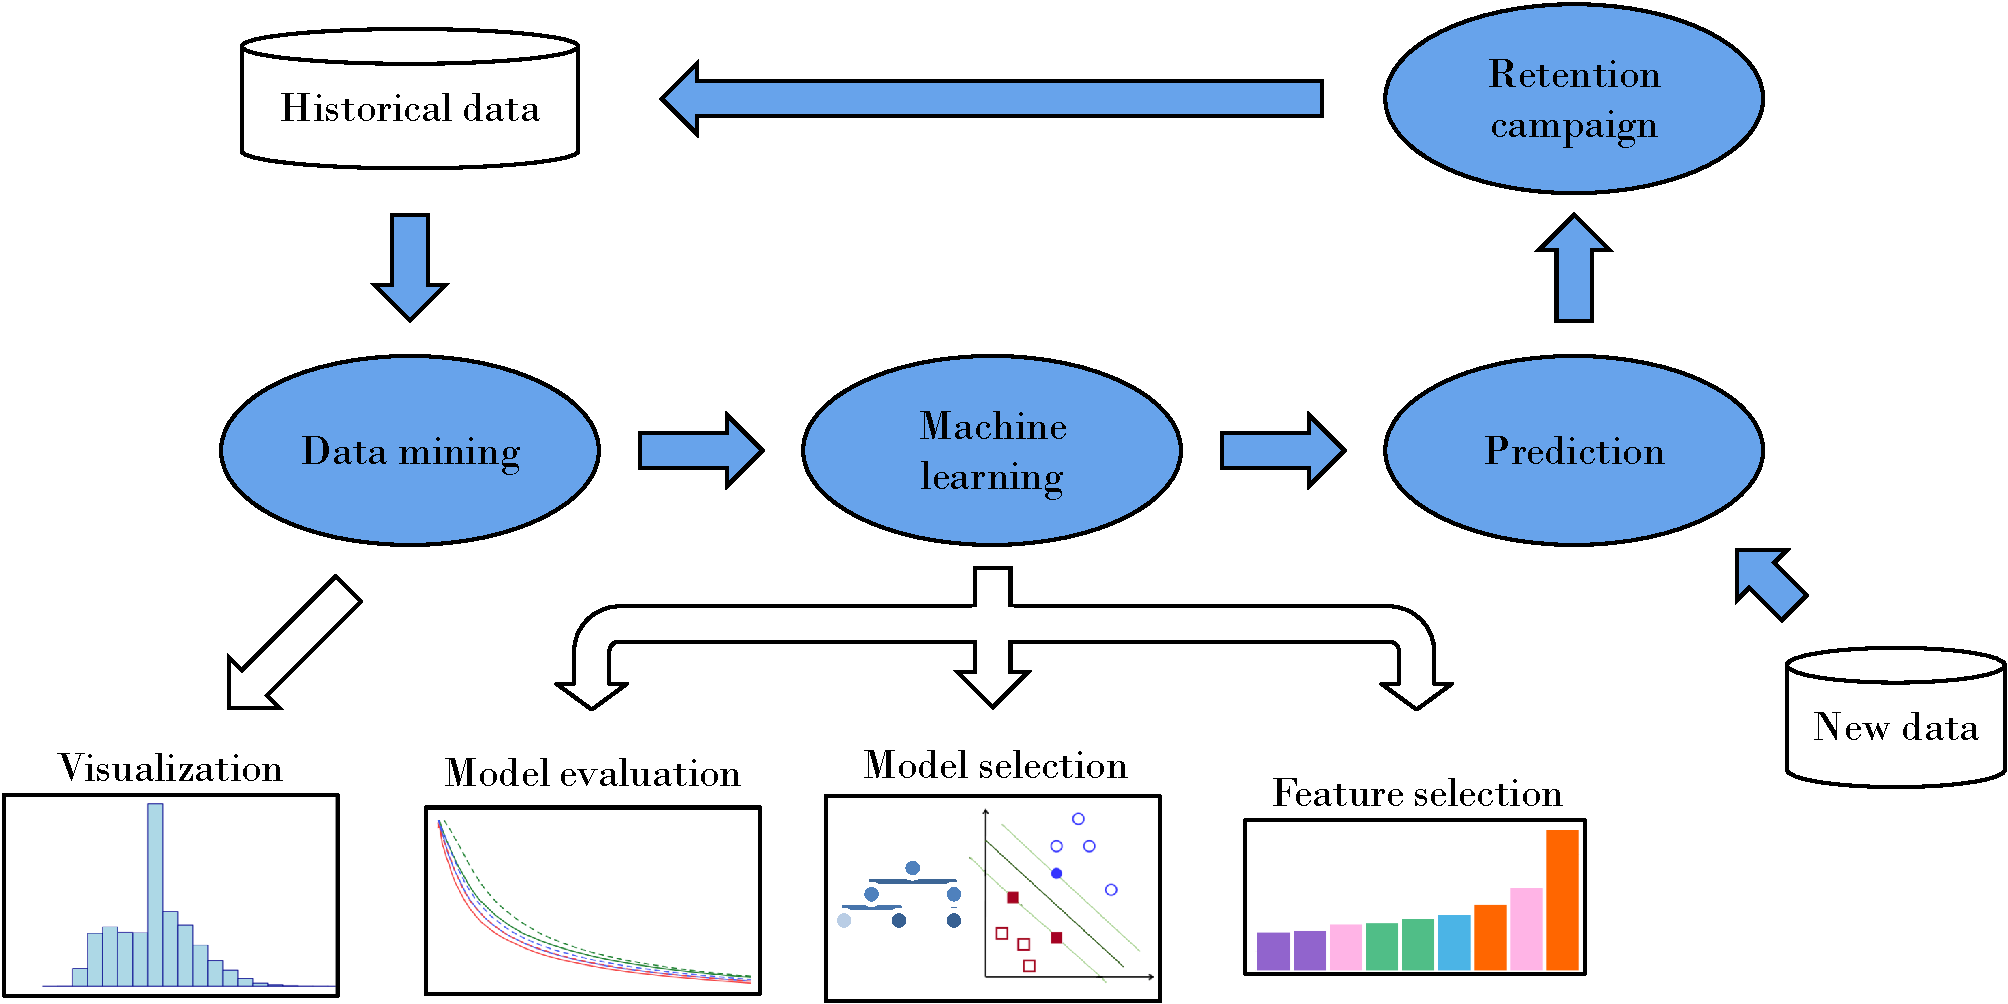
\includegraphics[width=0.8\linewidth]{figures/churn_diagram}
    \caption{The churn prevention process implemented at Orange.}
    \label{churn_diagram}
\end{figure}

The churn prevention process (depicted in figure \ref{churn_diagram}) starts by
collecting data about the customers and creating a \emph{historical database}.
This data summarizes the calls, messages, internet usage and other actions
performed by the customers. It also includes information about the subscription,
such as the type of tariff plan, its price, the subscription date, and so on.
Finally, personal data provided by the customer may as well be used, such as the
age or the place of residence. \emph{Data mining} is then used to provide a
quantitative understanding of the customers and their overall behavior. In
particular, the difference between churners and non-churners can be highlighted.
This is useful to decide which type of machine learning procedure should be used
for churn prediction, but can also bring valuable knowledge to marketing and
customer relationship teams. Once the data is sufficiently understood, a set of
relevant \emph{machine learning} models are built. These models learn from the
historical data the patterns typically exhibited by clients that will churn in
the near future. The types of patterns being learned, the techniques used to find
them, and the underlying assumptions are dependent on the model under
consideration. For example, a \emph{naive Bayes classifier} assumes that each
variable contributes to the probability of churn independently of the other
variables. In order to decide which model should be selected, the performances
of each model are compared by testing them on data left out of the training
phase. Feature selection is also performed, and consists in evaluating the
importance of each variable for predicting churn and training the model by
using only the most important ones. This reduces the computation time, and
generally improves the performances of the model since this reduces the noise
unimportant variables bring along. Once an efficient model has been selected,
the latest customer data is  submitted to the model, which outputs a probability
of churn for each customer. By ordering the customers by churn probability, a
list of the riskiest customers is established and sent to the campaigning team.
They split this set of clients into a \emph{target group} and a \emph{control
group}. Each customer of the target group is offered an incentive either by
phone call, email or message, while the control group is left untouched. This
allows, a few months later, to evaluate the impact of the retention campaign by
assessing the difference of churn rate in retrospective in the two groups.

\section{Causal inference}

Depending on the resources available and the techniques used, this data mining
pipeline can successfully predict potential churners, therefore allowing to
conduct targeted retention campaigns. But campaigners are then faced with
another challenge: what should they propose to the selected customers? Indeed,
the predictions given by data mining algorithms usually just consist in a
probability of churn. This prediction therefore does not indicate \emph{why} the
customer is about to stop her subscription. We need different analysis tools to
tackle this problem. This is the purpose of \emph{causal inference}, which is a
formal approach to find the causes of some event in a system. Causal inference
is usually conducted through \emph{controlled randomized experiments}, but the
scope of this master thesis did not allow such experiments. We therefore focus
on data-driven approaches, which are based on some properties of the statistical
distribution of causally linked variable.

To give an example of how causal inference can be conducted without experiment,
consider the simplistic world where two tariff plans are available, an expensive
one and a cheap one. The expensive plan makes customers consume more data per
month, and increases their probability to churn. We represent such causal
scenario with a \emph{directed acyclic graph} as in figure \ref{simple_causal}.
We plotted the data usage against the probability of churn for each tariff plan
in figure \ref{simple_causal_plot}. A positive correlation can be observed
between data usage and churn, but disappears when considering each tariff plan
separately. If a causal relationship also existed between data usage and churn
probability, the correlation would still be visible, even when conditioning on
the tariff plan. This idea of conditioning to discard putative causal links is
at the basis of most causal inference algorithms.

Such inference methods are based on a number of assumptions, such as the absence
of confounding factor. This assumption would be violated if, in our previous
example, the age of the customer influences both its choice of tariff plan and
its propensity  to churn. The causal inference algorithm would still conclude
that the expensive tariff plan causes clients to churn, while in reality they
churn solely because of their young age. This sort of erroneous conclusions can
lead to ineffective action in retention campaigns. Other inference methods imply
other assumptions, and care must be exercised when using them.

\begin{figure}
    \centering
    \begin{tikzpicture}
        \begin{scope}[every node/.style={ellipse,thick,draw}]
            \node (1) at (0, 0) {Tariff plan};
            \node[below left = of 1] (2) {Data usage};
            \node[below right = of 1] (3) {Churn};
        \end{scope}
        \begin{scope}[>={Stealth[black]},
            every edge/.style={draw=black,very thick}]
            \path [->] (1) edge node {} (3);
            \path [->] (1) edge node {} (2);
        \end{scope}
    \end{tikzpicture}
    \caption{Toy example of a causal diagram.}
    \label{simple_causal}
\end{figure}

\begin{figure}
    \centering
    % Created by tikzDevice version 0.12 on 2019-04-22 16:51:04
% !TEX encoding = UTF-8 Unicode
\begin{tikzpicture}[x=1pt,y=1pt]
\definecolor{fillColor}{RGB}{255,255,255}
\path[use as bounding box,fill=fillColor,fill opacity=0.00] (0,0) rectangle (289.08,216.81);
\begin{scope}
\path[clip] (  0.00,  0.00) rectangle (289.08,216.81);
\definecolor{drawColor}{RGB}{255,255,255}
\definecolor{fillColor}{RGB}{255,255,255}

\path[draw=drawColor,line width= 0.6pt,line join=round,line cap=round,fill=fillColor] (  0.00,  0.00) rectangle (289.08,216.81);
\end{scope}
\begin{scope}
\path[clip] ( 38.36, 30.72) rectangle (202.84,211.31);
\definecolor{fillColor}{RGB}{255,255,255}

\path[fill=fillColor] ( 38.36, 30.72) rectangle (202.84,211.31);
\definecolor{drawColor}{RGB}{236,144,92}

\path[draw=drawColor,line width= 0.4pt,line join=round,line cap=round] (147.98,193.93) --
	(150.62,189.35) --
	(145.34,189.35) --
	(147.98,193.93);

\path[draw=drawColor,line width= 0.4pt,line join=round,line cap=round] (174.34,194.68) --
	(176.98,190.11) --
	(171.69,190.11) --
	(174.34,194.68);
\definecolor{drawColor}{RGB}{68,107,154}

\path[draw=drawColor,line width= 0.4pt,line join=round,line cap=round] ( 69.18, 86.52) circle (  1.96);

\path[draw=drawColor,line width= 0.4pt,line join=round,line cap=round] ( 90.06, 55.58) circle (  1.96);

\path[draw=drawColor,line width= 0.4pt,line join=round,line cap=round] ( 99.51,109.18) circle (  1.96);

\path[draw=drawColor,line width= 0.4pt,line join=round,line cap=round] ( 78.65, 58.16) circle (  1.96);

\path[draw=drawColor,line width= 0.4pt,line join=round,line cap=round] ( 83.03,157.22) circle (  1.96);
\definecolor{drawColor}{RGB}{236,144,92}

\path[draw=drawColor,line width= 0.4pt,line join=round,line cap=round] (177.60,125.85) --
	(180.24,121.27) --
	(174.96,121.27) --
	(177.60,125.85);
\definecolor{drawColor}{RGB}{68,107,154}

\path[draw=drawColor,line width= 0.4pt,line join=round,line cap=round] ( 97.34, 42.96) circle (  1.96);

\path[draw=drawColor,line width= 0.4pt,line join=round,line cap=round] ( 92.57, 41.44) circle (  1.96);
\definecolor{drawColor}{RGB}{236,144,92}

\path[draw=drawColor,line width= 0.4pt,line join=round,line cap=round] (164.21,179.75) --
	(166.86,175.18) --
	(161.57,175.18) --
	(164.21,179.75);
\definecolor{drawColor}{RGB}{68,107,154}

\path[draw=drawColor,line width= 0.4pt,line join=round,line cap=round] ( 68.70, 74.60) circle (  1.96);

\path[draw=drawColor,line width= 0.4pt,line join=round,line cap=round] ( 93.89, 81.36) circle (  1.96);

\path[draw=drawColor,line width= 0.4pt,line join=round,line cap=round] ( 93.34, 52.90) circle (  1.96);

\path[draw=drawColor,line width= 0.4pt,line join=round,line cap=round] ( 94.98, 65.55) circle (  1.96);

\path[draw=drawColor,line width= 0.4pt,line join=round,line cap=round] ( 93.56, 99.48) circle (  1.96);

\path[draw=drawColor,line width= 0.4pt,line join=round,line cap=round] (108.64, 99.53) circle (  1.96);

\path[draw=drawColor,line width= 0.4pt,line join=round,line cap=round] ( 82.90,112.31) circle (  1.96);
\definecolor{drawColor}{RGB}{236,144,92}

\path[draw=drawColor,line width= 0.4pt,line join=round,line cap=round] (150.52,198.95) --
	(153.16,194.37) --
	(147.88,194.37) --
	(150.52,198.95);
\definecolor{drawColor}{RGB}{68,107,154}

\path[draw=drawColor,line width= 0.4pt,line join=round,line cap=round] (104.34, 75.20) circle (  1.96);

\path[draw=drawColor,line width= 0.4pt,line join=round,line cap=round] (100.13, 79.29) circle (  1.96);
\definecolor{drawColor}{RGB}{236,144,92}

\path[draw=drawColor,line width= 0.4pt,line join=round,line cap=round] (127.38,198.05) --
	(130.02,193.47) --
	(124.74,193.47) --
	(127.38,198.05);
\definecolor{drawColor}{RGB}{68,107,154}

\path[draw=drawColor,line width= 0.4pt,line join=round,line cap=round] ( 77.10, 51.93) circle (  1.96);
\definecolor{drawColor}{RGB}{236,144,92}

\path[draw=drawColor,line width= 0.4pt,line join=round,line cap=round] (166.98,174.53) --
	(169.63,169.95) --
	(164.34,169.95) --
	(166.98,174.53);
\definecolor{drawColor}{RGB}{68,107,154}

\path[draw=drawColor,line width= 0.4pt,line join=round,line cap=round] (103.42,105.60) circle (  1.96);

\path[draw=drawColor,line width= 0.4pt,line join=round,line cap=round] ( 76.50, 86.56) circle (  1.96);
\definecolor{drawColor}{RGB}{236,144,92}

\path[draw=drawColor,line width= 0.4pt,line join=round,line cap=round] (139.30,132.91) --
	(141.94,128.34) --
	(136.65,128.34) --
	(139.30,132.91);

\path[draw=drawColor,line width= 0.4pt,line join=round,line cap=round] (167.97,109.13) --
	(170.61,104.56) --
	(165.33,104.56) --
	(167.97,109.13);

\path[draw=drawColor,line width= 0.4pt,line join=round,line cap=round] (156.53,191.75) --
	(159.18,187.18) --
	(153.89,187.18) --
	(156.53,191.75);
\definecolor{drawColor}{RGB}{68,107,154}

\path[draw=drawColor,line width= 0.4pt,line join=round,line cap=round] ( 80.37, 78.42) circle (  1.96);

\path[draw=drawColor,line width= 0.4pt,line join=round,line cap=round] (106.19, 61.88) circle (  1.96);
\definecolor{drawColor}{RGB}{236,144,92}

\path[draw=drawColor,line width= 0.4pt,line join=round,line cap=round] (132.98,182.83) --
	(135.62,178.25) --
	(130.33,178.25) --
	(132.98,182.83);
\definecolor{drawColor}{RGB}{68,107,154}

\path[draw=drawColor,line width= 0.4pt,line join=round,line cap=round] ( 86.79, 64.24) circle (  1.96);
\definecolor{drawColor}{RGB}{236,144,92}

\path[draw=drawColor,line width= 0.4pt,line join=round,line cap=round] (133.80,172.21) --
	(136.44,167.64) --
	(131.16,167.64) --
	(133.80,172.21);
\definecolor{drawColor}{RGB}{68,107,154}

\path[draw=drawColor,line width= 0.4pt,line join=round,line cap=round] (112.18,130.69) circle (  1.96);

\path[draw=drawColor,line width= 0.4pt,line join=round,line cap=round] (107.86, 58.88) circle (  1.96);
\definecolor{drawColor}{RGB}{236,144,92}

\path[draw=drawColor,line width= 0.4pt,line join=round,line cap=round] (156.71,200.47) --
	(159.35,195.90) --
	(154.07,195.90) --
	(156.71,200.47);
\definecolor{drawColor}{RGB}{68,107,154}

\path[draw=drawColor,line width= 0.4pt,line join=round,line cap=round] ( 80.98, 88.11) circle (  1.96);
\definecolor{drawColor}{RGB}{236,144,92}

\path[draw=drawColor,line width= 0.4pt,line join=round,line cap=round] (174.06,203.41) --
	(176.71,198.83) --
	(171.42,198.83) --
	(174.06,203.41);
\definecolor{drawColor}{RGB}{68,107,154}

\path[draw=drawColor,line width= 0.4pt,line join=round,line cap=round] ( 80.81, 41.85) circle (  1.96);

\path[draw=drawColor,line width= 0.4pt,line join=round,line cap=round] (104.54,112.35) circle (  1.96);
\definecolor{drawColor}{RGB}{236,144,92}

\path[draw=drawColor,line width= 0.4pt,line join=round,line cap=round] (125.22,179.08) --
	(127.86,174.51) --
	(122.58,174.51) --
	(125.22,179.08);

\path[draw=drawColor,line width= 0.4pt,line join=round,line cap=round] (140.58,202.54) --
	(143.22,197.97) --
	(137.94,197.97) --
	(140.58,202.54);

\path[draw=drawColor,line width= 0.4pt,line join=round,line cap=round] (152.93,132.96) --
	(155.57,128.38) --
	(150.28,128.38) --
	(152.93,132.96);
\definecolor{drawColor}{RGB}{68,107,154}

\path[draw=drawColor,line width= 0.4pt,line join=round,line cap=round] (119.04, 47.24) circle (  1.96);
\definecolor{drawColor}{RGB}{236,144,92}

\path[draw=drawColor,line width= 0.4pt,line join=round,line cap=round] (173.24,145.55) --
	(175.88,140.98) --
	(170.59,140.98) --
	(173.24,145.55);
\definecolor{drawColor}{RGB}{68,107,154}

\path[draw=drawColor,line width= 0.4pt,line join=round,line cap=round] ( 76.83, 71.63) circle (  1.96);

\path[draw=drawColor,line width= 0.4pt,line join=round,line cap=round] (128.28, 42.30) circle (  1.96);

\path[draw=drawColor,line width= 0.4pt,line join=round,line cap=round] (113.20,102.14) circle (  1.96);

\path[draw=drawColor,line width= 0.4pt,line join=round,line cap=round] ( 64.25,117.85) circle (  1.96);

\path[draw=drawColor,line width= 0.4pt,line join=round,line cap=round] (121.39, 77.66) circle (  1.96);

\path[draw=drawColor,line width= 0.4pt,line join=round,line cap=round] ( 98.68, 71.96) circle (  1.96);

\path[draw=drawColor,line width= 0.4pt,line join=round,line cap=round] (103.09, 99.82) circle (  1.96);

\path[draw=drawColor,line width= 0.4pt,line join=round,line cap=round] ( 82.38, 59.81) circle (  1.96);

\path[draw=drawColor,line width= 0.4pt,line join=round,line cap=round] (100.64, 69.92) circle (  1.96);
\definecolor{drawColor}{RGB}{236,144,92}

\path[draw=drawColor,line width= 0.4pt,line join=round,line cap=round] (153.88,142.32) --
	(156.52,137.74) --
	(151.24,137.74) --
	(153.88,142.32);
\definecolor{drawColor}{RGB}{68,107,154}

\path[draw=drawColor,line width= 0.4pt,line join=round,line cap=round] (100.26, 77.77) circle (  1.96);

\path[draw=drawColor,line width= 0.4pt,line join=round,line cap=round] ( 84.19,117.89) circle (  1.96);

\path[draw=drawColor,line width= 0.4pt,line join=round,line cap=round] ( 72.43,112.28) circle (  1.96);

\path[draw=drawColor,line width= 0.4pt,line join=round,line cap=round] (110.19, 83.85) circle (  1.96);

\path[draw=drawColor,line width= 0.4pt,line join=round,line cap=round] ( 94.92, 68.31) circle (  1.96);
\definecolor{drawColor}{RGB}{236,144,92}

\path[draw=drawColor,line width= 0.4pt,line join=round,line cap=round] (186.63,164.04) --
	(189.27,159.47) --
	(183.99,159.47) --
	(186.63,164.04);
\definecolor{drawColor}{RGB}{68,107,154}

\path[draw=drawColor,line width= 0.4pt,line join=round,line cap=round] ( 89.37, 86.03) circle (  1.96);

\path[draw=drawColor,line width= 0.4pt,line join=round,line cap=round] ( 82.71, 59.87) circle (  1.96);

\path[draw=drawColor,line width= 0.4pt,line join=round,line cap=round] (105.97, 82.53) circle (  1.96);
\definecolor{drawColor}{RGB}{236,144,92}

\path[draw=drawColor,line width= 0.4pt,line join=round,line cap=round] (138.93,154.75) --
	(141.57,150.18) --
	(136.28,150.18) --
	(138.93,154.75);

\path[draw=drawColor,line width= 0.4pt,line join=round,line cap=round] (173.38,196.81) --
	(176.02,192.23) --
	(170.74,192.23) --
	(173.38,196.81);
\definecolor{drawColor}{RGB}{68,107,154}

\path[draw=drawColor,line width= 0.4pt,line join=round,line cap=round] ( 86.74,112.68) circle (  1.96);

\path[draw=drawColor,line width= 0.4pt,line join=round,line cap=round] ( 86.67,114.46) circle (  1.96);

\path[draw=drawColor,line width= 0.4pt,line join=round,line cap=round] ( 68.06, 59.17) circle (  1.96);

\path[draw=drawColor,line width= 0.4pt,line join=round,line cap=round] (104.01,115.00) circle (  1.96);

\path[draw=drawColor,line width= 0.4pt,line join=round,line cap=round] ( 85.02, 60.71) circle (  1.96);

\path[draw=drawColor,line width= 0.4pt,line join=round,line cap=round] ( 83.43, 63.14) circle (  1.96);

\path[draw=drawColor,line width= 0.4pt,line join=round,line cap=round] (115.70,108.36) circle (  1.96);

\path[draw=drawColor,line width= 0.4pt,line join=round,line cap=round] (108.25,126.65) circle (  1.96);

\path[draw=drawColor,line width= 0.4pt,line join=round,line cap=round] ( 79.84,110.33) circle (  1.96);

\path[draw=drawColor,line width= 0.4pt,line join=round,line cap=round] (103.26, 50.40) circle (  1.96);
\definecolor{drawColor}{RGB}{236,144,92}

\path[draw=drawColor,line width= 0.4pt,line join=round,line cap=round] (147.88,137.85) --
	(150.52,133.28) --
	(145.23,133.28) --
	(147.88,137.85);
\definecolor{drawColor}{RGB}{68,107,154}

\path[draw=drawColor,line width= 0.4pt,line join=round,line cap=round] ( 84.71, 75.31) circle (  1.96);
\definecolor{drawColor}{RGB}{236,144,92}

\path[draw=drawColor,line width= 0.4pt,line join=round,line cap=round] (189.37,139.91) --
	(192.01,135.33) --
	(186.73,135.33) --
	(189.37,139.91);
\definecolor{drawColor}{RGB}{68,107,154}

\path[draw=drawColor,line width= 0.4pt,line join=round,line cap=round] ( 84.13, 88.06) circle (  1.96);

\path[draw=drawColor,line width= 0.4pt,line join=round,line cap=round] ( 66.52, 76.57) circle (  1.96);

\path[draw=drawColor,line width= 0.4pt,line join=round,line cap=round] (101.24,129.04) circle (  1.96);
\definecolor{drawColor}{RGB}{236,144,92}

\path[draw=drawColor,line width= 0.4pt,line join=round,line cap=round] (158.23,162.70) --
	(160.87,158.12) --
	(155.59,158.12) --
	(158.23,162.70);

\path[draw=drawColor,line width= 0.4pt,line join=round,line cap=round] (162.98,177.81) --
	(165.63,173.23) --
	(160.34,173.23) --
	(162.98,177.81);
\definecolor{drawColor}{RGB}{68,107,154}

\path[draw=drawColor,line width= 0.4pt,line join=round,line cap=round] ( 99.17, 86.25) circle (  1.96);

\path[draw=drawColor,line width= 0.4pt,line join=round,line cap=round] (125.46, 53.50) circle (  1.96);

\path[draw=drawColor,line width= 0.4pt,line join=round,line cap=round] (104.73, 98.81) circle (  1.96);

\path[draw=drawColor,line width= 0.4pt,line join=round,line cap=round] ( 94.89, 91.36) circle (  1.96);

\path[draw=drawColor,line width= 0.4pt,line join=round,line cap=round] ( 98.06,110.19) circle (  1.96);
\definecolor{drawColor}{RGB}{236,144,92}

\path[draw=drawColor,line width= 0.4pt,line join=round,line cap=round] (172.49,172.35) --
	(175.14,167.77) --
	(169.85,167.77) --
	(172.49,172.35);

\path[draw=drawColor,line width= 0.4pt,line join=round,line cap=round] (166.70,185.13) --
	(169.34,180.55) --
	(164.06,180.55) --
	(166.70,185.13);
\definecolor{drawColor}{RGB}{68,107,154}

\path[draw=drawColor,line width= 0.4pt,line join=round,line cap=round] (110.31, 68.12) circle (  1.96);

\path[draw=drawColor,line width= 0.4pt,line join=round,line cap=round] ( 64.16,162.14) circle (  1.96);

\path[draw=drawColor,line width= 0.4pt,line join=round,line cap=round] ( 87.98, 79.57) circle (  1.96);

\path[draw=drawColor,line width= 0.4pt,line join=round,line cap=round] (110.13, 97.27) circle (  1.96);
\definecolor{drawColor}{RGB}{236,144,92}

\path[draw=drawColor,line width= 0.4pt,line join=round,line cap=round] (137.69,186.50) --
	(140.34,181.92) --
	(135.05,181.92) --
	(137.69,186.50);
\definecolor{drawColor}{RGB}{68,107,154}

\path[draw=drawColor,line width= 0.4pt,line join=round,line cap=round] ( 59.07,123.43) circle (  1.96);
\definecolor{drawColor}{RGB}{236,144,92}

\path[draw=drawColor,line width= 0.4pt,line join=round,line cap=round] (148.03,167.80) --
	(150.68,163.22) --
	(145.39,163.22) --
	(148.03,167.80);

\path[draw=drawColor,line width= 0.4pt,line join=round,line cap=round] (146.01,181.53) --
	(148.66,176.95) --
	(143.37,176.95) --
	(146.01,181.53);
\definecolor{drawColor}{RGB}{68,107,154}

\path[draw=drawColor,line width= 0.4pt,line join=round,line cap=round] (109.59, 67.70) circle (  1.96);
\definecolor{drawColor}{RGB}{236,144,92}

\path[draw=drawColor,line width= 0.4pt,line join=round,line cap=round] (133.45,137.89) --
	(136.09,133.32) --
	(130.80,133.32) --
	(133.45,137.89);
\definecolor{drawColor}{RGB}{68,107,154}

\path[draw=drawColor,line width= 0.4pt,line join=round,line cap=round] (107.48, 44.07) circle (  1.96);

\path[draw=drawColor,line width= 0.4pt,line join=round,line cap=round] (115.91, 95.76) circle (  1.96);

\path[draw=drawColor,line width= 0.4pt,line join=round,line cap=round] (102.57, 85.79) circle (  1.96);
\definecolor{drawColor}{RGB}{236,144,92}

\path[draw=drawColor,line width= 0.4pt,line join=round,line cap=round] (187.98,156.54) --
	(190.62,151.97) --
	(185.33,151.97) --
	(187.98,156.54);
\definecolor{drawColor}{RGB}{68,107,154}

\path[draw=drawColor,line width= 0.4pt,line join=round,line cap=round] ( 56.87,138.66) circle (  1.96);

\path[draw=drawColor,line width= 0.4pt,line join=round,line cap=round] (117.99, 62.39) circle (  1.96);
\definecolor{drawColor}{RGB}{236,144,92}

\path[draw=drawColor,line width= 0.4pt,line join=round,line cap=round] (159.77,190.16) --
	(162.41,185.59) --
	(157.13,185.59) --
	(159.77,190.16);
\definecolor{drawColor}{RGB}{68,107,154}

\path[draw=drawColor,line width= 0.4pt,line join=round,line cap=round] ( 93.52, 87.06) circle (  1.96);
\definecolor{drawColor}{RGB}{236,144,92}

\path[draw=drawColor,line width= 0.4pt,line join=round,line cap=round] (175.41,187.75) --
	(178.05,183.17) --
	(172.77,183.17) --
	(175.41,187.75);
\definecolor{drawColor}{RGB}{68,107,154}

\path[draw=drawColor,line width= 0.4pt,line join=round,line cap=round] ( 90.69, 75.52) circle (  1.96);

\path[draw=drawColor,line width= 0.4pt,line join=round,line cap=round] (106.93, 50.88) circle (  1.96);
\definecolor{drawColor}{RGB}{236,144,92}

\path[draw=drawColor,line width= 0.4pt,line join=round,line cap=round] (137.79,186.93) --
	(140.43,182.35) --
	(135.15,182.35) --
	(137.79,186.93);

\path[draw=drawColor,line width= 0.4pt,line join=round,line cap=round] (149.48,168.20) --
	(152.12,163.63) --
	(146.84,163.63) --
	(149.48,168.20);

\path[draw=drawColor,line width= 0.4pt,line join=round,line cap=round] (178.98,162.55) --
	(181.62,157.97) --
	(176.34,157.97) --
	(178.98,162.55);
\definecolor{drawColor}{RGB}{68,107,154}

\path[draw=drawColor,line width= 0.4pt,line join=round,line cap=round] ( 76.77, 48.71) circle (  1.96);
\definecolor{drawColor}{RGB}{236,144,92}

\path[draw=drawColor,line width= 0.4pt,line join=round,line cap=round] (157.35,182.08) --
	(159.99,177.50) --
	(154.71,177.50) --
	(157.35,182.08);

\path[draw=drawColor,line width= 0.4pt,line join=round,line cap=round] (183.79,149.47) --
	(186.44,144.89) --
	(181.15,144.89) --
	(183.79,149.47);
\definecolor{drawColor}{RGB}{68,107,154}

\path[draw=drawColor,line width= 0.4pt,line join=round,line cap=round] ( 77.79, 72.44) circle (  1.96);

\path[draw=drawColor,line width= 0.4pt,line join=round,line cap=round] (103.19, 94.29) circle (  1.96);

\path[draw=drawColor,line width= 0.4pt,line join=round,line cap=round] ( 95.02, 51.74) circle (  1.96);
\definecolor{drawColor}{RGB}{236,144,92}

\path[draw=drawColor,line width= 0.4pt,line join=round,line cap=round] (161.12,153.03) --
	(163.76,148.46) --
	(158.48,148.46) --
	(161.12,153.03);
\definecolor{drawColor}{RGB}{68,107,154}

\path[draw=drawColor,line width= 0.4pt,line join=round,line cap=round] ( 85.20, 76.98) circle (  1.96);

\path[draw=drawColor,line width= 0.4pt,line join=round,line cap=round] (100.40, 91.38) circle (  1.96);

\path[draw=drawColor,line width= 0.4pt,line join=round,line cap=round] ( 89.79, 52.99) circle (  1.96);

\path[draw=drawColor,line width= 0.4pt,line join=round,line cap=round] ( 90.42, 47.07) circle (  1.96);

\path[draw=drawColor,line width= 0.4pt,line join=round,line cap=round] ( 64.49,104.28) circle (  1.96);

\path[draw=drawColor,line width= 0.4pt,line join=round,line cap=round] ( 98.71, 65.94) circle (  1.96);

\path[draw=drawColor,line width= 0.4pt,line join=round,line cap=round] ( 84.92, 69.22) circle (  1.96);

\path[draw=drawColor,line width= 0.4pt,line join=round,line cap=round] ( 79.80,110.66) circle (  1.96);

\path[draw=drawColor,line width= 0.4pt,line join=round,line cap=round] ( 89.47, 78.47) circle (  1.96);

\path[draw=drawColor,line width= 0.4pt,line join=round,line cap=round] (103.38, 61.13) circle (  1.96);

\path[draw=drawColor,line width= 0.4pt,line join=round,line cap=round] ( 77.16,130.63) circle (  1.96);

\path[draw=drawColor,line width= 0.4pt,line join=round,line cap=round] (108.08,104.74) circle (  1.96);

\path[draw=drawColor,line width= 0.4pt,line join=round,line cap=round] (116.63, 49.07) circle (  1.96);

\path[draw=drawColor,line width= 0.4pt,line join=round,line cap=round] ( 72.31,128.85) circle (  1.96);

\path[draw=drawColor,line width= 0.4pt,line join=round,line cap=round] ( 82.01, 71.76) circle (  1.96);

\path[draw=drawColor,line width= 0.4pt,line join=round,line cap=round] ( 93.16, 59.07) circle (  1.96);

\path[draw=drawColor,line width= 0.4pt,line join=round,line cap=round] ( 95.27, 96.13) circle (  1.96);

\path[draw=drawColor,line width= 0.4pt,line join=round,line cap=round] ( 96.06, 71.12) circle (  1.96);

\path[draw=drawColor,line width= 0.4pt,line join=round,line cap=round] ( 77.07,103.27) circle (  1.96);

\path[draw=drawColor,line width= 0.4pt,line join=round,line cap=round] (111.86, 64.19) circle (  1.96);

\path[draw=drawColor,line width= 0.4pt,line join=round,line cap=round] (119.19, 72.18) circle (  1.96);

\path[draw=drawColor,line width= 0.4pt,line join=round,line cap=round] ( 99.99, 76.34) circle (  1.96);
\definecolor{drawColor}{RGB}{236,144,92}

\path[draw=drawColor,line width= 0.4pt,line join=round,line cap=round] (145.51,174.65) --
	(148.16,170.07) --
	(142.87,170.07) --
	(145.51,174.65);
\definecolor{drawColor}{RGB}{68,107,154}

\path[draw=drawColor,line width= 0.4pt,line join=round,line cap=round] ( 89.48, 73.75) circle (  1.96);

\path[draw=drawColor,line width= 0.4pt,line join=round,line cap=round] ( 89.21, 81.07) circle (  1.96);

\path[draw=drawColor,line width= 0.4pt,line join=round,line cap=round] (101.33, 86.51) circle (  1.96);

\path[draw=drawColor,line width= 0.4pt,line join=round,line cap=round] ( 77.74, 57.69) circle (  1.96);

\path[draw=drawColor,line width= 0.4pt,line join=round,line cap=round] ( 89.88, 72.52) circle (  1.96);

\path[draw=drawColor,line width= 0.4pt,line join=round,line cap=round] ( 94.11,113.89) circle (  1.96);
\definecolor{drawColor}{RGB}{236,144,92}

\path[draw=drawColor,line width= 0.4pt,line join=round,line cap=round] (177.39,179.02) --
	(180.04,174.44) --
	(174.75,174.44) --
	(177.39,179.02);
\definecolor{drawColor}{RGB}{68,107,154}

\path[draw=drawColor,line width= 0.4pt,line join=round,line cap=round] (130.27,118.80) circle (  1.96);

\path[draw=drawColor,line width= 0.4pt,line join=round,line cap=round] (107.67, 90.05) circle (  1.96);

\path[draw=drawColor,line width= 0.4pt,line join=round,line cap=round] ( 93.89,116.69) circle (  1.96);
\definecolor{drawColor}{RGB}{236,144,92}

\path[draw=drawColor,line width= 0.4pt,line join=round,line cap=round] (152.51,147.27) --
	(155.16,142.70) --
	(149.87,142.70) --
	(152.51,147.27);
\definecolor{drawColor}{RGB}{68,107,154}

\path[draw=drawColor,line width= 0.4pt,line join=round,line cap=round] (106.15,125.85) circle (  1.96);

\path[draw=drawColor,line width= 0.4pt,line join=round,line cap=round] ( 95.79, 55.31) circle (  1.96);
\definecolor{drawColor}{RGB}{236,144,92}

\path[draw=drawColor,line width= 0.4pt,line join=round,line cap=round] (159.56,154.32) --
	(162.20,149.74) --
	(156.91,149.74) --
	(159.56,154.32);
\definecolor{drawColor}{RGB}{68,107,154}

\path[draw=drawColor,line width= 0.4pt,line join=round,line cap=round] ( 94.42, 56.46) circle (  1.96);

\path[draw=drawColor,line width= 0.4pt,line join=round,line cap=round] (104.00, 77.33) circle (  1.96);

\path[draw=drawColor,line width= 0.4pt,line join=round,line cap=round] (103.69, 64.29) circle (  1.96);

\path[draw=drawColor,line width= 0.4pt,line join=round,line cap=round] ( 83.47,113.53) circle (  1.96);

\path[draw=drawColor,line width= 0.4pt,line join=round,line cap=round] ( 89.15, 84.03) circle (  1.96);

\path[draw=drawColor,line width= 0.4pt,line join=round,line cap=round] ( 96.53, 70.74) circle (  1.96);

\path[draw=drawColor,line width= 0.4pt,line join=round,line cap=round] (108.93, 59.92) circle (  1.96);
\definecolor{drawColor}{RGB}{236,144,92}

\path[draw=drawColor,line width= 0.4pt,line join=round,line cap=round] (149.01,153.12) --
	(151.65,148.54) --
	(146.37,148.54) --
	(149.01,153.12);
\definecolor{drawColor}{RGB}{68,107,154}

\path[draw=drawColor,line width= 0.4pt,line join=round,line cap=round] (106.66, 85.60) circle (  1.96);

\path[draw=drawColor,line width= 0.4pt,line join=round,line cap=round] ( 96.77,118.61) circle (  1.96);

\path[draw=drawColor,line width= 0.4pt,line join=round,line cap=round] (102.85,101.68) circle (  1.96);

\path[draw=drawColor,line width= 0.4pt,line join=round,line cap=round] ( 83.55, 78.83) circle (  1.96);
\definecolor{drawColor}{RGB}{236,144,92}

\path[draw=drawColor,line width= 0.4pt,line join=round,line cap=round] (172.65,132.68) --
	(175.29,128.11) --
	(170.01,128.11) --
	(172.65,132.68);
\definecolor{drawColor}{RGB}{68,107,154}

\path[draw=drawColor,line width= 0.4pt,line join=round,line cap=round] ( 91.64, 74.66) circle (  1.96);

\path[draw=drawColor,line width= 0.4pt,line join=round,line cap=round] ( 85.03,130.01) circle (  1.96);
\definecolor{drawColor}{RGB}{236,144,92}

\path[draw=drawColor,line width= 0.4pt,line join=round,line cap=round] (170.47,202.81) --
	(173.11,198.23) --
	(167.83,198.23) --
	(170.47,202.81);
\definecolor{drawColor}{RGB}{68,107,154}

\path[draw=drawColor,line width= 0.4pt,line join=round,line cap=round] ( 78.62, 57.72) circle (  1.96);

\path[draw=drawColor,line width= 0.4pt,line join=round,line cap=round] (122.06, 90.48) circle (  1.96);

\path[draw=drawColor,line width= 0.4pt,line join=round,line cap=round] (102.82,100.06) circle (  1.96);

\path[draw=drawColor,line width= 0.4pt,line join=round,line cap=round] ( 98.45,110.20) circle (  1.96);

\path[draw=drawColor,line width= 0.4pt,line join=round,line cap=round] ( 90.31,112.73) circle (  1.96);

\path[draw=drawColor,line width= 0.4pt,line join=round,line cap=round] ( 74.21,101.81) circle (  1.96);

\path[draw=drawColor,line width= 0.4pt,line join=round,line cap=round] ( 78.42,100.95) circle (  1.96);
\definecolor{drawColor}{RGB}{236,144,92}

\path[draw=drawColor,line width= 0.4pt,line join=round,line cap=round] (158.09,172.86) --
	(160.73,168.28) --
	(155.45,168.28) --
	(158.09,172.86);
\definecolor{drawColor}{RGB}{68,107,154}

\path[draw=drawColor,line width= 0.4pt,line join=round,line cap=round] ( 82.71, 75.85) circle (  1.96);
\definecolor{drawColor}{RGB}{236,144,92}

\path[draw=drawColor,line width= 0.4pt,line join=round,line cap=round] (165.81,134.93) --
	(168.45,130.35) --
	(163.17,130.35) --
	(165.81,134.93);

\path[draw=drawColor,line width= 0.4pt,line join=round,line cap=round] (169.62,182.83) --
	(172.27,178.25) --
	(166.98,178.25) --
	(169.62,182.83);
\definecolor{drawColor}{RGB}{68,107,154}

\path[draw=drawColor,line width= 0.4pt,line join=round,line cap=round] ( 92.50, 94.58) circle (  1.96);

\path[draw=drawColor,line width= 0.4pt,line join=round,line cap=round] ( 83.32,156.21) circle (  1.96);

\path[draw=drawColor,line width= 0.4pt,line join=round,line cap=round] ( 85.16, 59.25) circle (  1.96);
\definecolor{drawColor}{RGB}{236,144,92}

\path[draw=drawColor,line width= 0.4pt,line join=round,line cap=round] (168.21,154.10) --
	(170.85,149.52) --
	(165.56,149.52) --
	(168.21,154.10);

\path[draw=drawColor,line width= 0.4pt,line join=round,line cap=round] (145.50,117.91) --
	(148.15,113.33) --
	(142.86,113.33) --
	(145.50,117.91);
\definecolor{drawColor}{RGB}{68,107,154}

\path[draw=drawColor,line width= 0.4pt,line join=round,line cap=round] ( 84.17, 83.04) circle (  1.96);

\path[draw=drawColor,line width= 0.4pt,line join=round,line cap=round] (112.13,102.96) circle (  1.96);

\path[draw=drawColor,line width= 0.4pt,line join=round,line cap=round] ( 91.46,101.50) circle (  1.96);

\path[draw=drawColor,line width= 0.4pt,line join=round,line cap=round] ( 84.57, 76.87) circle (  1.96);

\path[draw=drawColor,line width= 0.4pt,line join=round,line cap=round] (123.21,108.44) circle (  1.96);

\path[draw=drawColor,line width= 0.4pt,line join=round,line cap=round] ( 92.29, 82.29) circle (  1.96);

\path[draw=drawColor,line width= 0.4pt,line join=round,line cap=round] (124.08, 80.64) circle (  1.96);

\path[draw=drawColor,line width= 0.4pt,line join=round,line cap=round] ( 96.93,110.36) circle (  1.96);

\path[draw=drawColor,line width= 0.4pt,line join=round,line cap=round] (106.15, 66.04) circle (  1.96);

\path[draw=drawColor,line width= 0.4pt,line join=round,line cap=round] ( 91.73,122.82) circle (  1.96);
\definecolor{drawColor}{RGB}{236,144,92}

\path[draw=drawColor,line width= 0.4pt,line join=round,line cap=round] (171.35,173.68) --
	(173.99,169.11) --
	(168.71,169.11) --
	(171.35,173.68);

\path[draw=drawColor,line width= 0.4pt,line join=round,line cap=round] (172.05,188.71) --
	(174.69,184.14) --
	(169.41,184.14) --
	(172.05,188.71);
\definecolor{drawColor}{RGB}{68,107,154}

\path[draw=drawColor,line width= 0.4pt,line join=round,line cap=round] (112.62,158.65) circle (  1.96);
\definecolor{drawColor}{RGB}{236,144,92}

\path[draw=drawColor,line width= 0.4pt,line join=round,line cap=round] (147.79, 89.37) --
	(150.43, 84.80) --
	(145.15, 84.80) --
	(147.79, 89.37);
\definecolor{drawColor}{RGB}{68,107,154}

\path[draw=drawColor,line width= 0.4pt,line join=round,line cap=round] (106.71, 50.94) circle (  1.96);
\definecolor{drawColor}{RGB}{236,144,92}

\path[draw=drawColor,line width= 0.4pt,line join=round,line cap=round] (150.90,115.40) --
	(153.54,110.82) --
	(148.26,110.82) --
	(150.90,115.40);
\definecolor{drawColor}{RGB}{68,107,154}

\path[draw=drawColor,line width= 0.4pt,line join=round,line cap=round] ( 89.20, 57.51) circle (  1.96);

\path[draw=drawColor,line width= 0.4pt,line join=round,line cap=round] ( 78.02,105.39) circle (  1.96);

\path[draw=drawColor,line width= 0.4pt,line join=round,line cap=round] (117.22, 55.42) circle (  1.96);

\path[draw=drawColor,line width= 0.4pt,line join=round,line cap=round] ( 99.35, 82.36) circle (  1.96);

\path[draw=drawColor,line width= 0.4pt,line join=round,line cap=round] ( 93.89,101.05) circle (  1.96);

\path[draw=drawColor,line width= 0.4pt,line join=round,line cap=round] (109.21, 50.32) circle (  1.96);

\path[draw=drawColor,line width= 0.4pt,line join=round,line cap=round] ( 88.17, 47.09) circle (  1.96);

\path[draw=drawColor,line width= 0.4pt,line join=round,line cap=round] (106.75, 98.03) circle (  1.96);
\definecolor{drawColor}{RGB}{236,144,92}

\path[draw=drawColor,line width= 0.4pt,line join=round,line cap=round] (157.71,173.78) --
	(160.36,169.20) --
	(155.07,169.20) --
	(157.71,173.78);
\definecolor{drawColor}{RGB}{68,107,154}

\path[draw=drawColor,line width= 0.4pt,line join=round,line cap=round] (110.54, 45.35) circle (  1.96);
\definecolor{drawColor}{RGB}{236,144,92}

\path[draw=drawColor,line width= 0.4pt,line join=round,line cap=round] (144.51,195.66) --
	(147.15,191.08) --
	(141.87,191.08) --
	(144.51,195.66);
\definecolor{drawColor}{RGB}{68,107,154}

\path[draw=drawColor,line width= 0.4pt,line join=round,line cap=round] (110.41, 55.29) circle (  1.96);

\path[draw=drawColor,line width= 0.4pt,line join=round,line cap=round] ( 87.55, 70.05) circle (  1.96);
\definecolor{drawColor}{RGB}{236,144,92}

\path[draw=drawColor,line width= 0.4pt,line join=round,line cap=round] (195.37,174.74) --
	(198.01,170.16) --
	(192.72,170.16) --
	(195.37,174.74);
\definecolor{drawColor}{RGB}{68,107,154}

\path[draw=drawColor,line width= 0.4pt,line join=round,line cap=round] ( 84.39, 64.44) circle (  1.96);

\path[draw=drawColor,line width= 0.4pt,line join=round,line cap=round] ( 92.99, 81.99) circle (  1.96);

\path[draw=drawColor,line width= 0.4pt,line join=round,line cap=round] ( 69.82, 77.09) circle (  1.96);
\definecolor{drawColor}{RGB}{236,144,92}

\path[draw=drawColor,line width= 0.4pt,line join=round,line cap=round] (147.94, 98.70) --
	(150.58, 94.12) --
	(145.29, 94.12) --
	(147.94, 98.70);
\definecolor{drawColor}{RGB}{68,107,154}

\path[draw=drawColor,line width= 0.4pt,line join=round,line cap=round] ( 81.19, 92.86) circle (  1.96);
\definecolor{drawColor}{RGB}{236,144,92}

\path[draw=drawColor,line width= 0.4pt,line join=round,line cap=round] (149.06,150.87) --
	(151.70,146.29) --
	(146.42,146.29) --
	(149.06,150.87);
\definecolor{drawColor}{RGB}{68,107,154}

\path[draw=drawColor,line width= 0.4pt,line join=round,line cap=round] ( 95.22, 60.94) circle (  1.96);

\path[draw=drawColor,line width= 0.4pt,line join=round,line cap=round] ( 81.51, 50.99) circle (  1.96);

\path[draw=drawColor,line width= 0.4pt,line join=round,line cap=round] (125.12, 46.52) circle (  1.96);
\definecolor{drawColor}{RGB}{236,144,92}

\path[draw=drawColor,line width= 0.4pt,line join=round,line cap=round] (156.56,200.14) --
	(159.20,195.56) --
	(153.92,195.56) --
	(156.56,200.14);
\definecolor{drawColor}{RGB}{68,107,154}

\path[draw=drawColor,line width= 0.4pt,line join=round,line cap=round] (104.15, 71.28) circle (  1.96);

\path[draw=drawColor,line width= 0.4pt,line join=round,line cap=round] ( 93.64, 66.51) circle (  1.96);

\path[draw=drawColor,line width= 0.4pt,line join=round,line cap=round] (105.81, 72.59) circle (  1.96);

\path[draw=drawColor,line width= 0.4pt,line join=round,line cap=round] ( 77.41, 96.32) circle (  1.96);

\path[draw=drawColor,line width= 0.4pt,line join=round,line cap=round] ( 90.78,108.08) circle (  1.96);

\path[draw=drawColor,line width= 0.4pt,line join=round,line cap=round] ( 76.93,131.23) circle (  1.96);

\path[draw=drawColor,line width= 0.4pt,line join=round,line cap=round] ( 78.22, 65.37) circle (  1.96);

\path[draw=drawColor,line width= 0.4pt,line join=round,line cap=round] ( 96.00, 59.64) circle (  1.96);
\definecolor{drawColor}{RGB}{236,144,92}

\path[draw=drawColor,line width= 0.4pt,line join=round,line cap=round] (190.14,131.60) --
	(192.78,127.03) --
	(187.50,127.03) --
	(190.14,131.60);
\definecolor{drawColor}{RGB}{68,107,154}

\path[draw=drawColor,line width= 0.4pt,line join=round,line cap=round] (111.61,137.01) circle (  1.96);

\path[draw=drawColor,line width= 0.4pt,line join=round,line cap=round] (116.77, 94.51) circle (  1.96);

\path[draw=drawColor,line width= 0.4pt,line join=round,line cap=round] ( 95.81, 95.58) circle (  1.96);

\path[draw=drawColor,line width= 0.4pt,line join=round,line cap=round] ( 91.66,120.18) circle (  1.96);

\path[draw=drawColor,line width= 0.4pt,line join=round,line cap=round] (102.00,101.31) circle (  1.96);

\path[draw=drawColor,line width= 0.4pt,line join=round,line cap=round] ( 82.40,127.48) circle (  1.96);

\path[draw=drawColor,line width= 0.4pt,line join=round,line cap=round] ( 78.08, 94.34) circle (  1.96);
\definecolor{drawColor}{RGB}{236,144,92}

\path[draw=drawColor,line width= 0.4pt,line join=round,line cap=round] (163.51,164.98) --
	(166.15,160.40) --
	(160.87,160.40) --
	(163.51,164.98);
\definecolor{drawColor}{RGB}{68,107,154}

\path[draw=drawColor,line width= 0.4pt,line join=round,line cap=round] ( 83.68, 53.45) circle (  1.96);

\path[draw=drawColor,line width= 0.4pt,line join=round,line cap=round] (106.35,113.67) circle (  1.96);

\path[draw=drawColor,line width= 0.4pt,line join=round,line cap=round] ( 86.39, 63.38) circle (  1.96);

\path[draw=drawColor,line width= 0.4pt,line join=round,line cap=round] ( 82.44, 97.59) circle (  1.96);

\path[draw=drawColor,line width= 0.4pt,line join=round,line cap=round] ( 75.85,126.15) circle (  1.96);
\definecolor{drawColor}{RGB}{236,144,92}

\path[draw=drawColor,line width= 0.4pt,line join=round,line cap=round] (123.04,132.52) --
	(125.68,127.94) --
	(120.40,127.94) --
	(123.04,132.52);

\path[draw=drawColor,line width= 0.4pt,line join=round,line cap=round] (153.88,129.16) --
	(156.52,124.58) --
	(151.24,124.58) --
	(153.88,129.16);
\definecolor{drawColor}{RGB}{68,107,154}

\path[draw=drawColor,line width= 0.4pt,line join=round,line cap=round] (106.38, 68.75) circle (  1.96);
\definecolor{drawColor}{RGB}{236,144,92}

\path[draw=drawColor,line width= 0.4pt,line join=round,line cap=round] (153.53,159.03) --
	(156.17,154.45) --
	(150.89,154.45) --
	(153.53,159.03);

\path[draw=drawColor,line width= 0.4pt,line join=round,line cap=round] (153.43,129.95) --
	(156.08,125.38) --
	(150.79,125.38) --
	(153.43,129.95);
\definecolor{drawColor}{RGB}{68,107,154}

\path[draw=drawColor,line width= 0.4pt,line join=round,line cap=round] ( 69.92,100.18) circle (  1.96);

\path[draw=drawColor,line width= 0.4pt,line join=round,line cap=round] ( 84.70,121.88) circle (  1.96);

\path[draw=drawColor,line width= 0.4pt,line join=round,line cap=round] ( 78.18,141.55) circle (  1.96);

\path[draw=drawColor,line width= 0.4pt,line join=round,line cap=round] ( 99.84, 67.84) circle (  1.96);

\path[draw=drawColor,line width= 0.4pt,line join=round,line cap=round] ( 86.39, 76.89) circle (  1.96);
\definecolor{drawColor}{RGB}{236,144,92}

\path[draw=drawColor,line width= 0.4pt,line join=round,line cap=round] (161.51,185.44) --
	(164.16,180.86) --
	(158.87,180.86) --
	(161.51,185.44);
\definecolor{drawColor}{RGB}{68,107,154}

\path[draw=drawColor,line width= 0.4pt,line join=round,line cap=round] ( 78.70,131.39) circle (  1.96);

\path[draw=drawColor,line width= 0.4pt,line join=round,line cap=round] ( 72.73, 85.41) circle (  1.96);
\definecolor{drawColor}{RGB}{236,144,92}

\path[draw=drawColor,line width= 0.4pt,line join=round,line cap=round] (138.13,176.31) --
	(140.77,171.74) --
	(135.48,171.74) --
	(138.13,176.31);
\definecolor{drawColor}{RGB}{68,107,154}

\path[draw=drawColor,line width= 0.4pt,line join=round,line cap=round] ( 83.09, 82.46) circle (  1.96);

\path[draw=drawColor,line width= 0.4pt,line join=round,line cap=round] (108.45, 88.73) circle (  1.96);

\path[draw=drawColor,line width= 0.4pt,line join=round,line cap=round] (109.47, 65.92) circle (  1.96);

\path[draw=drawColor,line width= 0.4pt,line join=round,line cap=round] (120.18,136.53) circle (  1.96);

\path[draw=drawColor,line width= 0.4pt,line join=round,line cap=round] ( 94.95,102.78) circle (  1.96);

\path[draw=drawColor,line width= 0.4pt,line join=round,line cap=round] (122.49, 99.10) circle (  1.96);

\path[draw=drawColor,line width= 0.4pt,line join=round,line cap=round] ( 78.57, 87.55) circle (  1.96);

\path[draw=drawColor,line width= 0.4pt,line join=round,line cap=round] ( 96.33,135.76) circle (  1.96);
\definecolor{drawColor}{RGB}{236,144,92}

\path[draw=drawColor,line width= 0.4pt,line join=round,line cap=round] (148.51,161.88) --
	(151.15,157.30) --
	(145.87,157.30) --
	(148.51,161.88);
\definecolor{drawColor}{RGB}{68,107,154}

\path[draw=drawColor,line width= 0.4pt,line join=round,line cap=round] (117.44, 91.50) circle (  1.96);

\path[draw=drawColor,line width= 0.4pt,line join=round,line cap=round] (111.94, 53.77) circle (  1.96);

\path[draw=drawColor,line width= 0.4pt,line join=round,line cap=round] (106.41, 83.46) circle (  1.96);

\path[draw=drawColor,line width= 0.4pt,line join=round,line cap=round] ( 95.34, 61.27) circle (  1.96);
\definecolor{drawColor}{RGB}{236,144,92}

\path[draw=drawColor,line width= 0.4pt,line join=round,line cap=round] (144.56,191.97) --
	(147.20,187.39) --
	(141.92,187.39) --
	(144.56,191.97);

\path[draw=drawColor,line width= 0.4pt,line join=round,line cap=round] (177.79,177.92) --
	(180.43,173.35) --
	(175.15,173.35) --
	(177.79,177.92);
\definecolor{drawColor}{RGB}{68,107,154}

\path[draw=drawColor,line width= 0.4pt,line join=round,line cap=round] ( 81.50, 76.83) circle (  1.96);

\path[draw=drawColor,line width= 0.4pt,line join=round,line cap=round] ( 88.48,141.54) circle (  1.96);

\path[draw=drawColor,line width= 0.4pt,line join=round,line cap=round] ( 80.55, 51.65) circle (  1.96);

\path[draw=drawColor,line width= 0.4pt,line join=round,line cap=round] ( 93.12, 50.85) circle (  1.96);

\path[draw=drawColor,line width= 0.4pt,line join=round,line cap=round] ( 80.23, 87.16) circle (  1.96);
\definecolor{drawColor}{RGB}{236,144,92}

\path[draw=drawColor,line width= 0.4pt,line join=round,line cap=round] (174.01,124.36) --
	(176.66,119.78) --
	(171.37,119.78) --
	(174.01,124.36);
\definecolor{drawColor}{RGB}{68,107,154}

\path[draw=drawColor,line width= 0.4pt,line join=round,line cap=round] ( 98.00, 95.05) circle (  1.96);

\path[draw=drawColor,line width= 0.4pt,line join=round,line cap=round] (106.11, 88.45) circle (  1.96);

\path[draw=drawColor,line width= 0.4pt,line join=round,line cap=round] (122.87, 66.11) circle (  1.96);

\path[draw=drawColor,line width= 0.4pt,line join=round,line cap=round] (121.26, 78.03) circle (  1.96);

\path[draw=drawColor,line width= 0.4pt,line join=round,line cap=round] ( 91.82, 69.38) circle (  1.96);

\path[draw=drawColor,line width= 0.4pt,line join=round,line cap=round] ( 78.43,114.36) circle (  1.96);
\definecolor{drawColor}{RGB}{236,144,92}

\path[draw=drawColor,line width= 0.4pt,line join=round,line cap=round] (158.34,189.25) --
	(160.98,184.68) --
	(155.69,184.68) --
	(158.34,189.25);

\path[draw=drawColor,line width= 0.4pt,line join=round,line cap=round] (160.82,151.53) --
	(163.46,146.95) --
	(158.17,146.95) --
	(160.82,151.53);
\definecolor{drawColor}{RGB}{68,107,154}

\path[draw=drawColor,line width= 0.4pt,line join=round,line cap=round] ( 61.56, 75.52) circle (  1.96);
\definecolor{drawColor}{RGB}{236,144,92}

\path[draw=drawColor,line width= 0.4pt,line join=round,line cap=round] (170.55,148.40) --
	(173.19,143.82) --
	(167.90,143.82) --
	(170.55,148.40);
\definecolor{drawColor}{RGB}{68,107,154}

\path[draw=drawColor,line width= 0.4pt,line join=round,line cap=round] ( 84.34, 98.78) circle (  1.96);
\definecolor{drawColor}{RGB}{236,144,92}

\path[draw=drawColor,line width= 0.4pt,line join=round,line cap=round] (140.13, 79.08) --
	(142.77, 74.50) --
	(137.48, 74.50) --
	(140.13, 79.08);
\definecolor{drawColor}{RGB}{68,107,154}

\path[draw=drawColor,line width= 0.4pt,line join=round,line cap=round] ( 98.72, 41.74) circle (  1.96);

\path[draw=drawColor,line width= 0.4pt,line join=round,line cap=round] ( 87.54, 62.82) circle (  1.96);

\path[draw=drawColor,line width= 0.4pt,line join=round,line cap=round] (103.16,105.94) circle (  1.96);

\path[draw=drawColor,line width= 0.4pt,line join=round,line cap=round] ( 86.98, 98.98) circle (  1.96);

\path[draw=drawColor,line width= 0.4pt,line join=round,line cap=round] ( 94.90, 65.42) circle (  1.96);

\path[draw=drawColor,line width= 0.4pt,line join=round,line cap=round] ( 99.67,110.34) circle (  1.96);

\path[draw=drawColor,line width= 0.4pt,line join=round,line cap=round] (100.52, 48.12) circle (  1.96);

\path[draw=drawColor,line width= 0.4pt,line join=round,line cap=round] ( 73.87, 66.13) circle (  1.96);

\path[draw=drawColor,line width= 0.4pt,line join=round,line cap=round] ( 61.48,118.17) circle (  1.96);

\path[draw=drawColor,line width= 0.4pt,line join=round,line cap=round] ( 81.24, 56.96) circle (  1.96);
\definecolor{drawColor}{RGB}{236,144,92}

\path[draw=drawColor,line width= 0.4pt,line join=round,line cap=round] (159.20,200.28) --
	(161.85,195.71) --
	(156.56,195.71) --
	(159.20,200.28);
\definecolor{drawColor}{RGB}{68,107,154}

\path[draw=drawColor,line width= 0.4pt,line join=round,line cap=round] (106.37, 92.61) circle (  1.96);

\path[draw=drawColor,line width= 0.4pt,line join=round,line cap=round] ( 84.86,115.87) circle (  1.96);
\definecolor{drawColor}{RGB}{236,144,92}

\path[draw=drawColor,line width= 0.4pt,line join=round,line cap=round] (160.72,130.14) --
	(163.37,125.56) --
	(158.08,125.56) --
	(160.72,130.14);

\path[draw=drawColor,line width= 0.4pt,line join=round,line cap=round] (178.80,185.13) --
	(181.44,180.55) --
	(176.16,180.55) --
	(178.80,185.13);

\path[draw=drawColor,line width= 0.4pt,line join=round,line cap=round] (168.69,162.30) --
	(171.34,157.72) --
	(166.05,157.72) --
	(168.69,162.30);
\definecolor{drawColor}{RGB}{68,107,154}

\path[draw=drawColor,line width= 0.4pt,line join=round,line cap=round] ( 82.18, 83.99) circle (  1.96);
\definecolor{drawColor}{RGB}{236,144,92}

\path[draw=drawColor,line width= 0.4pt,line join=round,line cap=round] (158.23,166.50) --
	(160.88,161.92) --
	(155.59,161.92) --
	(158.23,166.50);
\definecolor{drawColor}{RGB}{68,107,154}

\path[draw=drawColor,line width= 0.4pt,line join=round,line cap=round] ( 85.40,100.91) circle (  1.96);

\path[draw=drawColor,line width= 0.4pt,line join=round,line cap=round] ( 98.05, 72.63) circle (  1.96);
\definecolor{drawColor}{RGB}{236,144,92}

\path[draw=drawColor,line width= 0.4pt,line join=round,line cap=round] (164.80,178.07) --
	(167.44,173.49) --
	(162.16,173.49) --
	(164.80,178.07);
\definecolor{drawColor}{RGB}{68,107,154}

\path[draw=drawColor,line width= 0.4pt,line join=round,line cap=round] (102.91, 74.27) circle (  1.96);

\path[draw=drawColor,line width= 0.4pt,line join=round,line cap=round] ( 89.68,117.35) circle (  1.96);
\definecolor{drawColor}{RGB}{236,144,92}

\path[draw=drawColor,line width= 0.4pt,line join=round,line cap=round] (167.31,160.53) --
	(169.95,155.95) --
	(164.67,155.95) --
	(167.31,160.53);
\definecolor{drawColor}{RGB}{68,107,154}

\path[draw=drawColor,line width= 0.4pt,line join=round,line cap=round] (107.53, 74.45) circle (  1.96);
\definecolor{drawColor}{RGB}{236,144,92}

\path[draw=drawColor,line width= 0.4pt,line join=round,line cap=round] (157.46,197.09) --
	(160.10,192.51) --
	(154.82,192.51) --
	(157.46,197.09);
\definecolor{drawColor}{RGB}{68,107,154}

\path[draw=drawColor,line width= 0.4pt,line join=round,line cap=round] ( 78.60, 71.51) circle (  1.96);
\definecolor{drawColor}{RGB}{236,144,92}

\path[draw=drawColor,line width= 0.4pt,line join=round,line cap=round] (155.26,183.21) --
	(157.90,178.63) --
	(152.62,178.63) --
	(155.26,183.21);
\definecolor{drawColor}{RGB}{68,107,154}

\path[draw=drawColor,line width= 0.4pt,line join=round,line cap=round] ( 74.97, 52.55) circle (  1.96);

\path[draw=drawColor,line width= 0.4pt,line join=round,line cap=round] ( 72.78, 66.33) circle (  1.96);

\path[draw=drawColor,line width= 0.4pt,line join=round,line cap=round] (105.84,117.05) circle (  1.96);
\definecolor{drawColor}{RGB}{236,144,92}

\path[draw=drawColor,line width= 0.4pt,line join=round,line cap=round] (155.66,140.10) --
	(158.30,135.52) --
	(153.01,135.52) --
	(155.66,140.10);

\path[draw=drawColor,line width= 0.4pt,line join=round,line cap=round] (145.50,106.01) --
	(148.14,101.44) --
	(142.85,101.44) --
	(145.50,106.01);
\definecolor{drawColor}{RGB}{68,107,154}

\path[draw=drawColor,line width= 0.4pt,line join=round,line cap=round] (101.49, 49.94) circle (  1.96);
\definecolor{drawColor}{RGB}{236,144,92}

\path[draw=drawColor,line width= 0.4pt,line join=round,line cap=round] (154.33,164.14) --
	(156.97,159.56) --
	(151.68,159.56) --
	(154.33,164.14);
\definecolor{drawColor}{RGB}{68,107,154}

\path[draw=drawColor,line width= 0.4pt,line join=round,line cap=round] ( 87.95, 74.21) circle (  1.96);

\path[draw=drawColor,line width= 0.4pt,line join=round,line cap=round] ( 89.78, 71.29) circle (  1.96);

\path[draw=drawColor,line width= 0.4pt,line join=round,line cap=round] ( 90.39, 84.85) circle (  1.96);

\path[draw=drawColor,line width= 0.4pt,line join=round,line cap=round] (131.95,115.02) circle (  1.96);

\path[draw=drawColor,line width= 0.4pt,line join=round,line cap=round] ( 64.20,101.69) circle (  1.96);

\path[draw=drawColor,line width= 0.4pt,line join=round,line cap=round] ( 80.65, 60.03) circle (  1.96);

\path[draw=drawColor,line width= 0.4pt,line join=round,line cap=round] (100.54,119.92) circle (  1.96);

\path[draw=drawColor,line width= 0.4pt,line join=round,line cap=round] (109.34,136.33) circle (  1.96);
\definecolor{drawColor}{RGB}{236,144,92}

\path[draw=drawColor,line width= 0.4pt,line join=round,line cap=round] (149.93,159.45) --
	(152.57,154.87) --
	(147.29,154.87) --
	(149.93,159.45);

\path[draw=drawColor,line width= 0.4pt,line join=round,line cap=round] (147.58,125.69) --
	(150.22,121.11) --
	(144.94,121.11) --
	(147.58,125.69);
\definecolor{drawColor}{RGB}{68,107,154}

\path[draw=drawColor,line width= 0.4pt,line join=round,line cap=round] (115.25,110.12) circle (  1.96);

\path[draw=drawColor,line width= 0.4pt,line join=round,line cap=round] ( 74.78, 56.32) circle (  1.96);

\path[draw=drawColor,line width= 0.4pt,line join=round,line cap=round] ( 91.71, 76.17) circle (  1.96);

\path[draw=drawColor,line width= 0.4pt,line join=round,line cap=round] (105.51,119.89) circle (  1.96);

\path[draw=drawColor,line width= 0.4pt,line join=round,line cap=round] (106.47, 83.43) circle (  1.96);
\definecolor{drawColor}{RGB}{236,144,92}

\path[draw=drawColor,line width= 0.4pt,line join=round,line cap=round] (152.71,181.21) --
	(155.35,176.64) --
	(150.07,176.64) --
	(152.71,181.21);
\definecolor{drawColor}{RGB}{68,107,154}

\path[draw=drawColor,line width= 0.4pt,line join=round,line cap=round] (100.35, 71.70) circle (  1.96);

\path[draw=drawColor,line width= 0.4pt,line join=round,line cap=round] (103.52, 91.67) circle (  1.96);

\path[draw=drawColor,line width= 0.4pt,line join=round,line cap=round] (113.46, 67.99) circle (  1.96);

\path[draw=drawColor,line width= 0.4pt,line join=round,line cap=round] ( 80.51, 85.11) circle (  1.96);

\path[draw=drawColor,line width= 0.4pt,line join=round,line cap=round] (120.64, 72.80) circle (  1.96);
\definecolor{drawColor}{RGB}{236,144,92}

\path[draw=drawColor,line width= 0.4pt,line join=round,line cap=round] (169.66,183.35) --
	(172.30,178.78) --
	(167.02,178.78) --
	(169.66,183.35);

\path[draw=drawColor,line width= 0.4pt,line join=round,line cap=round] (145.18,160.96) --
	(147.82,156.38) --
	(142.54,156.38) --
	(145.18,160.96);
\definecolor{drawColor}{RGB}{68,107,154}

\path[draw=drawColor,line width= 0.4pt,line join=round,line cap=round] ( 82.12,101.35) circle (  1.96);

\path[draw=drawColor,line width= 0.4pt,line join=round,line cap=round] (104.27,123.68) circle (  1.96);

\path[draw=drawColor,line width= 0.4pt,line join=round,line cap=round] ( 92.42, 86.93) circle (  1.96);
\definecolor{drawColor}{RGB}{236,144,92}

\path[draw=drawColor,line width= 0.4pt,line join=round,line cap=round] (151.25,139.77) --
	(153.89,135.20) --
	(148.61,135.20) --
	(151.25,139.77);

\path[draw=drawColor,line width= 0.4pt,line join=round,line cap=round] (149.16,179.71) --
	(151.80,175.13) --
	(146.52,175.13) --
	(149.16,179.71);
\definecolor{drawColor}{RGB}{68,107,154}

\path[draw=drawColor,line width= 0.4pt,line join=round,line cap=round] ( 76.24,103.12) circle (  1.96);

\path[draw=drawColor,line width= 0.4pt,line join=round,line cap=round] ( 83.66, 96.07) circle (  1.96);

\path[draw=drawColor,line width= 0.4pt,line join=round,line cap=round] (100.43, 90.24) circle (  1.96);

\path[draw=drawColor,line width= 0.4pt,line join=round,line cap=round] (116.39, 78.45) circle (  1.96);

\path[draw=drawColor,line width= 0.4pt,line join=round,line cap=round] (100.55, 50.09) circle (  1.96);

\path[draw=drawColor,line width= 0.4pt,line join=round,line cap=round] (105.72,108.29) circle (  1.96);

\path[draw=drawColor,line width= 0.4pt,line join=round,line cap=round] (111.35, 80.02) circle (  1.96);

\path[draw=drawColor,line width= 0.4pt,line join=round,line cap=round] (113.71, 70.64) circle (  1.96);

\path[draw=drawColor,line width= 0.4pt,line join=round,line cap=round] ( 63.62, 43.72) circle (  1.96);

\path[draw=drawColor,line width= 0.4pt,line join=round,line cap=round] ( 79.91, 73.01) circle (  1.96);

\path[draw=drawColor,line width= 0.4pt,line join=round,line cap=round] ( 89.92,134.95) circle (  1.96);

\path[draw=drawColor,line width= 0.4pt,line join=round,line cap=round] ( 99.84,106.70) circle (  1.96);
\definecolor{drawColor}{RGB}{236,144,92}

\path[draw=drawColor,line width= 0.4pt,line join=round,line cap=round] (159.24,168.06) --
	(161.89,163.48) --
	(156.60,163.48) --
	(159.24,168.06);
\definecolor{drawColor}{RGB}{68,107,154}

\path[draw=drawColor,line width= 0.4pt,line join=round,line cap=round] (103.62, 80.27) circle (  1.96);
\definecolor{drawColor}{RGB}{236,144,92}

\path[draw=drawColor,line width= 0.4pt,line join=round,line cap=round] (141.98,166.87) --
	(144.62,162.29) --
	(139.34,162.29) --
	(141.98,166.87);
\definecolor{drawColor}{RGB}{68,107,154}

\path[draw=drawColor,line width= 0.4pt,line join=round,line cap=round] (124.93,109.18) circle (  1.96);
\definecolor{drawColor}{RGB}{236,144,92}

\path[draw=drawColor,line width= 0.4pt,line join=round,line cap=round] (145.81,203.44) --
	(148.45,198.86) --
	(143.17,198.86) --
	(145.81,203.44);

\path[draw=drawColor,line width= 0.4pt,line join=round,line cap=round] (167.58,184.89) --
	(170.22,180.31) --
	(164.94,180.31) --
	(167.58,184.89);
\definecolor{drawColor}{RGB}{68,107,154}

\path[draw=drawColor,line width= 0.4pt,line join=round,line cap=round] ( 80.41, 80.35) circle (  1.96);

\path[draw=drawColor,line width= 0.4pt,line join=round,line cap=round] (125.62, 47.06) circle (  1.96);
\definecolor{drawColor}{RGB}{236,144,92}

\path[draw=drawColor,line width= 0.4pt,line join=round,line cap=round] (153.63,117.93) --
	(156.27,113.36) --
	(150.99,113.36) --
	(153.63,117.93);

\path[draw=drawColor,line width= 0.4pt,line join=round,line cap=round] (161.97,198.33) --
	(164.61,193.75) --
	(159.33,193.75) --
	(161.97,198.33);

\path[draw=drawColor,line width= 0.4pt,line join=round,line cap=round] (165.26,195.05) --
	(167.91,190.48) --
	(162.62,190.48) --
	(165.26,195.05);
\definecolor{drawColor}{RGB}{68,107,154}

\path[draw=drawColor,line width= 0.4pt,line join=round,line cap=round] ( 93.98, 88.49) circle (  1.96);

\path[draw=drawColor,line width= 0.4pt,line join=round,line cap=round] ( 86.75,111.44) circle (  1.96);

\path[draw=drawColor,line width= 0.4pt,line join=round,line cap=round] (103.10, 66.40) circle (  1.96);
\definecolor{drawColor}{RGB}{236,144,92}

\path[draw=drawColor,line width= 0.4pt,line join=round,line cap=round] (173.68,144.88) --
	(176.32,140.30) --
	(171.03,140.30) --
	(173.68,144.88);
\definecolor{drawColor}{RGB}{68,107,154}

\path[draw=drawColor,line width= 0.4pt,line join=round,line cap=round] ( 98.98, 52.02) circle (  1.96);

\path[draw=drawColor,line width= 0.4pt,line join=round,line cap=round] (111.04, 88.63) circle (  1.96);
\definecolor{drawColor}{RGB}{236,144,92}

\path[draw=drawColor,line width= 0.4pt,line join=round,line cap=round] (160.60,154.29) --
	(163.24,149.71) --
	(157.96,149.71) --
	(160.60,154.29);
\definecolor{drawColor}{RGB}{68,107,154}

\path[draw=drawColor,line width= 0.4pt,line join=round,line cap=round] ( 60.04, 65.93) circle (  1.96);
\definecolor{drawColor}{RGB}{236,144,92}

\path[draw=drawColor,line width= 0.4pt,line join=round,line cap=round] (147.44,152.36) --
	(150.08,147.78) --
	(144.80,147.78) --
	(147.44,152.36);

\path[draw=drawColor,line width= 0.4pt,line join=round,line cap=round] (159.86,113.31) --
	(162.50,108.73) --
	(157.22,108.73) --
	(159.86,113.31);
\definecolor{drawColor}{RGB}{68,107,154}

\path[draw=drawColor,line width= 0.4pt,line join=round,line cap=round] ( 83.02, 70.23) circle (  1.96);

\path[draw=drawColor,line width= 0.4pt,line join=round,line cap=round] ( 95.72,114.21) circle (  1.96);

\path[draw=drawColor,line width= 0.4pt,line join=round,line cap=round] (107.69, 69.14) circle (  1.96);

\path[draw=drawColor,line width= 0.4pt,line join=round,line cap=round] (104.21, 96.07) circle (  1.96);

\path[draw=drawColor,line width= 0.4pt,line join=round,line cap=round] ( 88.32,115.12) circle (  1.96);
\definecolor{drawColor}{RGB}{236,144,92}

\path[draw=drawColor,line width= 0.4pt,line join=round,line cap=round] (163.27,143.08) --
	(165.92,138.50) --
	(160.63,138.50) --
	(163.27,143.08);
\definecolor{drawColor}{RGB}{68,107,154}

\path[draw=drawColor,line width= 0.4pt,line join=round,line cap=round] (109.42, 90.39) circle (  1.96);

\path[draw=drawColor,line width= 0.4pt,line join=round,line cap=round] ( 95.03, 82.11) circle (  1.96);

\path[draw=drawColor,line width= 0.4pt,line join=round,line cap=round] (101.01, 80.19) circle (  1.96);

\path[draw=drawColor,line width= 0.4pt,line join=round,line cap=round] (102.93,138.33) circle (  1.96);

\path[draw=drawColor,line width= 0.4pt,line join=round,line cap=round] (132.46,121.68) circle (  1.96);
\definecolor{drawColor}{RGB}{236,144,92}

\path[draw=drawColor,line width= 0.4pt,line join=round,line cap=round] (163.37,135.05) --
	(166.01,130.47) --
	(160.73,130.47) --
	(163.37,135.05);
\definecolor{drawColor}{RGB}{68,107,154}

\path[draw=drawColor,line width= 0.4pt,line join=round,line cap=round] ( 96.93, 61.16) circle (  1.96);

\path[draw=drawColor,line width= 0.4pt,line join=round,line cap=round] (114.75,118.07) circle (  1.96);

\path[draw=drawColor,line width= 0.4pt,line join=round,line cap=round] ( 90.13, 58.01) circle (  1.96);

\path[draw=drawColor,line width= 0.4pt,line join=round,line cap=round] (101.56, 82.48) circle (  1.96);

\path[draw=drawColor,line width= 0.4pt,line join=round,line cap=round] ( 68.36, 69.78) circle (  1.96);

\path[draw=drawColor,line width= 0.4pt,line join=round,line cap=round] ( 93.47, 79.72) circle (  1.96);

\path[draw=drawColor,line width= 0.4pt,line join=round,line cap=round] ( 71.11, 68.30) circle (  1.96);

\path[draw=drawColor,line width= 0.4pt,line join=round,line cap=round] ( 87.14,168.29) circle (  1.96);

\path[draw=drawColor,line width= 0.4pt,line join=round,line cap=round] ( 77.40,133.71) circle (  1.96);

\path[draw=drawColor,line width= 0.4pt,line join=round,line cap=round] (117.49, 51.27) circle (  1.96);
\definecolor{drawColor}{RGB}{236,144,92}

\path[draw=drawColor,line width= 0.4pt,line join=round,line cap=round] (164.59,144.02) --
	(167.23,139.44) --
	(161.94,139.44) --
	(164.59,144.02);
\definecolor{drawColor}{RGB}{68,107,154}

\path[draw=drawColor,line width= 0.4pt,line join=round,line cap=round] ( 87.03, 82.99) circle (  1.96);
\definecolor{drawColor}{RGB}{236,144,92}

\path[draw=drawColor,line width= 0.4pt,line join=round,line cap=round] (155.18,170.24) --
	(157.82,165.67) --
	(152.53,165.67) --
	(155.18,170.24);
\definecolor{drawColor}{RGB}{68,107,154}

\path[draw=drawColor,line width= 0.4pt,line join=round,line cap=round] ( 65.91, 85.46) circle (  1.96);

\path[draw=drawColor,line width= 0.4pt,line join=round,line cap=round] ( 96.52, 86.66) circle (  1.96);

\path[draw=drawColor,line width= 0.4pt,line join=round,line cap=round] ( 85.22,159.74) circle (  1.96);
\definecolor{drawColor}{RGB}{236,144,92}

\path[draw=drawColor,line width= 0.4pt,line join=round,line cap=round] (160.85,114.20) --
	(163.49,109.63) --
	(158.21,109.63) --
	(160.85,114.20);

\path[draw=drawColor,line width= 0.4pt,line join=round,line cap=round] (167.30,195.53) --
	(169.94,190.95) --
	(164.66,190.95) --
	(167.30,195.53);

\path[draw=drawColor,line width= 0.4pt,line join=round,line cap=round] (176.99,139.23) --
	(179.63,134.65) --
	(174.34,134.65) --
	(176.99,139.23);
\definecolor{drawColor}{RGB}{68,107,154}

\path[draw=drawColor,line width= 0.4pt,line join=round,line cap=round] ( 89.03, 86.79) circle (  1.96);
\definecolor{drawColor}{RGB}{236,144,92}

\path[draw=drawColor,line width= 0.4pt,line join=round,line cap=round] (144.24,169.66) --
	(146.88,165.08) --
	(141.60,165.08) --
	(144.24,169.66);
\definecolor{drawColor}{RGB}{68,107,154}

\path[draw=drawColor,line width= 0.4pt,line join=round,line cap=round] (127.54, 59.28) circle (  1.96);

\path[draw=drawColor,line width= 0.4pt,line join=round,line cap=round] (105.43,128.67) circle (  1.96);
\definecolor{drawColor}{RGB}{236,144,92}

\path[draw=drawColor,line width= 0.4pt,line join=round,line cap=round] (142.27,165.74) --
	(144.92,161.16) --
	(139.63,161.16) --
	(142.27,165.74);

\path[draw=drawColor,line width= 0.4pt,line join=round,line cap=round] (134.83,119.20) --
	(137.47,114.62) --
	(132.19,114.62) --
	(134.83,119.20);
\definecolor{drawColor}{RGB}{68,107,154}

\path[draw=drawColor,line width= 0.4pt,line join=round,line cap=round] ( 76.08, 45.76) circle (  1.96);

\path[draw=drawColor,line width= 0.4pt,line join=round,line cap=round] ( 91.23, 82.74) circle (  1.96);

\path[draw=drawColor,line width= 0.4pt,line join=round,line cap=round] (136.04, 97.55) circle (  1.96);

\path[draw=drawColor,line width= 0.4pt,line join=round,line cap=round] (103.08, 79.95) circle (  1.96);

\path[draw=drawColor,line width= 0.4pt,line join=round,line cap=round] (105.66, 59.77) circle (  1.96);

\path[draw=drawColor,line width= 0.4pt,line join=round,line cap=round] ( 85.65, 60.04) circle (  1.96);
\definecolor{drawColor}{RGB}{236,144,92}

\path[draw=drawColor,line width= 0.4pt,line join=round,line cap=round] (176.26,176.11) --
	(178.90,171.53) --
	(173.62,171.53) --
	(176.26,176.11);
\definecolor{drawColor}{RGB}{68,107,154}

\path[draw=drawColor,line width= 0.4pt,line join=round,line cap=round] ( 95.32, 74.29) circle (  1.96);
\definecolor{drawColor}{RGB}{236,144,92}

\path[draw=drawColor,line width= 0.4pt,line join=round,line cap=round] (145.90,194.29) --
	(148.54,189.71) --
	(143.26,189.71) --
	(145.90,194.29);
\definecolor{drawColor}{RGB}{68,107,154}

\path[draw=drawColor,line width= 0.4pt,line join=round,line cap=round] (105.13,119.12) circle (  1.96);
\definecolor{drawColor}{RGB}{236,144,92}

\path[draw=drawColor,line width= 0.4pt,line join=round,line cap=round] (142.53,146.79) --
	(145.18,142.21) --
	(139.89,142.21) --
	(142.53,146.79);
\definecolor{drawColor}{RGB}{68,107,154}

\path[draw=drawColor,line width= 0.4pt,line join=round,line cap=round] ( 93.32, 82.12) circle (  1.96);

\path[draw=drawColor,line width= 0.4pt,line join=round,line cap=round] ( 75.80, 77.24) circle (  1.96);

\path[draw=drawColor,line width= 0.4pt,line join=round,line cap=round] ( 78.76,103.55) circle (  1.96);

\path[draw=drawColor,line width= 0.4pt,line join=round,line cap=round] (107.65,101.43) circle (  1.96);

\path[draw=drawColor,line width= 0.4pt,line join=round,line cap=round] ( 77.77, 62.22) circle (  1.96);

\path[draw=drawColor,line width= 0.4pt,line join=round,line cap=round] ( 82.74, 76.41) circle (  1.96);

\path[draw=drawColor,line width= 0.4pt,line join=round,line cap=round] ( 83.62, 68.85) circle (  1.96);

\path[draw=drawColor,line width= 0.4pt,line join=round,line cap=round] ( 60.84,114.91) circle (  1.96);
\definecolor{drawColor}{RGB}{236,144,92}

\path[draw=drawColor,line width= 0.4pt,line join=round,line cap=round] (146.64,187.67) --
	(149.28,183.09) --
	(143.99,183.09) --
	(146.64,187.67);
\definecolor{drawColor}{RGB}{68,107,154}

\path[draw=drawColor,line width= 0.4pt,line join=round,line cap=round] (105.85,145.17) circle (  1.96);
\definecolor{drawColor}{RGB}{236,144,92}

\path[draw=drawColor,line width= 0.4pt,line join=round,line cap=round] (165.40,189.06) --
	(168.04,184.48) --
	(162.76,184.48) --
	(165.40,189.06);
\definecolor{drawColor}{RGB}{68,107,154}

\path[draw=drawColor,line width= 0.4pt,line join=round,line cap=round] ( 83.38, 68.66) circle (  1.96);
\definecolor{drawColor}{RGB}{236,144,92}

\path[draw=drawColor,line width= 0.4pt,line join=round,line cap=round] (150.82,182.51) --
	(153.46,177.93) --
	(148.18,177.93) --
	(150.82,182.51);
\definecolor{drawColor}{RGB}{68,107,154}

\path[draw=drawColor,line width= 0.4pt,line join=round,line cap=round] ( 72.37, 84.73) circle (  1.96);
\definecolor{drawColor}{RGB}{236,144,92}

\path[draw=drawColor,line width= 0.4pt,line join=round,line cap=round] (159.88,183.07) --
	(162.53,178.49) --
	(157.24,178.49) --
	(159.88,183.07);
\definecolor{drawColor}{RGB}{68,107,154}

\path[draw=drawColor,line width= 0.4pt,line join=round,line cap=round] (112.65,107.71) circle (  1.96);

\path[draw=drawColor,line width= 0.4pt,line join=round,line cap=round] ( 69.21, 99.88) circle (  1.96);

\path[draw=drawColor,line width= 0.4pt,line join=round,line cap=round] (112.70,128.26) circle (  1.96);

\path[draw=drawColor,line width= 0.4pt,line join=round,line cap=round] ( 91.47, 73.56) circle (  1.96);

\path[draw=drawColor,line width= 0.4pt,line join=round,line cap=round] ( 87.68, 93.95) circle (  1.96);

\path[draw=drawColor,line width= 0.4pt,line join=round,line cap=round] ( 86.40,112.04) circle (  1.96);

\path[draw=drawColor,line width= 0.4pt,line join=round,line cap=round] ( 80.27, 73.55) circle (  1.96);
\definecolor{drawColor}{RGB}{236,144,92}

\path[draw=drawColor,line width= 0.4pt,line join=round,line cap=round] (164.68, 98.52) --
	(167.33, 93.94) --
	(162.04, 93.94) --
	(164.68, 98.52);
\definecolor{drawColor}{RGB}{68,107,154}

\path[draw=drawColor,line width= 0.4pt,line join=round,line cap=round] ( 86.57, 73.09) circle (  1.96);
\definecolor{drawColor}{RGB}{236,144,92}

\path[draw=drawColor,line width= 0.4pt,line join=round,line cap=round] (149.65,203.28) --
	(152.29,198.70) --
	(147.00,198.70) --
	(149.65,203.28);
\definecolor{drawColor}{RGB}{68,107,154}

\path[draw=drawColor,line width= 0.4pt,line join=round,line cap=round] ( 88.41, 57.46) circle (  1.96);

\path[draw=drawColor,line width= 0.4pt,line join=round,line cap=round] ( 97.08, 96.33) circle (  1.96);

\path[draw=drawColor,line width= 0.4pt,line join=round,line cap=round] (125.62, 77.26) circle (  1.96);

\path[draw=drawColor,line width= 0.4pt,line join=round,line cap=round] ( 98.38, 89.88) circle (  1.96);

\path[draw=drawColor,line width= 0.4pt,line join=round,line cap=round] ( 85.23, 75.76) circle (  1.96);

\path[draw=drawColor,line width= 0.4pt,line join=round,line cap=round] (135.14, 99.57) circle (  1.96);

\path[draw=drawColor,line width= 0.4pt,line join=round,line cap=round] ( 83.95, 75.63) circle (  1.96);

\path[draw=drawColor,line width= 0.4pt,line join=round,line cap=round] ( 89.65, 65.64) circle (  1.96);

\path[draw=drawColor,line width= 0.4pt,line join=round,line cap=round] (102.64, 54.16) circle (  1.96);
\definecolor{drawColor}{RGB}{236,144,92}

\path[draw=drawColor,line width= 0.4pt,line join=round,line cap=round] (151.79,154.72) --
	(154.43,150.14) --
	(149.14,150.14) --
	(151.79,154.72);
\definecolor{drawColor}{RGB}{68,107,154}

\path[draw=drawColor,line width= 0.4pt,line join=round,line cap=round] ( 91.42,100.95) circle (  1.96);

\path[draw=drawColor,line width= 0.4pt,line join=round,line cap=round] ( 65.67, 88.19) circle (  1.96);

\path[draw=drawColor,line width= 0.4pt,line join=round,line cap=round] ( 94.18,114.98) circle (  1.96);

\path[draw=drawColor,line width= 0.4pt,line join=round,line cap=round] ( 62.88, 50.52) circle (  1.96);

\path[draw=drawColor,line width= 0.4pt,line join=round,line cap=round] (121.59, 73.87) circle (  1.96);

\path[draw=drawColor,line width= 0.4pt,line join=round,line cap=round] (111.83, 58.00) circle (  1.96);
\definecolor{drawColor}{RGB}{236,144,92}

\path[draw=drawColor,line width= 0.4pt,line join=round,line cap=round] (129.68,137.25) --
	(132.32,132.68) --
	(127.03,132.68) --
	(129.68,137.25);
\definecolor{drawColor}{RGB}{68,107,154}

\path[draw=drawColor,line width= 0.4pt,line join=round,line cap=round] ( 91.90, 77.37) circle (  1.96);

\path[draw=drawColor,line width= 0.4pt,line join=round,line cap=round] (130.47, 74.96) circle (  1.96);
\definecolor{drawColor}{RGB}{236,144,92}

\path[draw=drawColor,line width= 0.4pt,line join=round,line cap=round] (156.64,206.15) --
	(159.28,201.58) --
	(153.99,201.58) --
	(156.64,206.15);
\definecolor{drawColor}{RGB}{68,107,154}

\path[draw=drawColor,line width= 0.4pt,line join=round,line cap=round] ( 56.10, 90.50) circle (  1.96);

\path[draw=drawColor,line width= 0.4pt,line join=round,line cap=round] ( 82.09, 86.35) circle (  1.96);
\definecolor{drawColor}{RGB}{236,144,92}

\path[draw=drawColor,line width= 0.4pt,line join=round,line cap=round] (169.31,188.03) --
	(171.95,183.45) --
	(166.66,183.45) --
	(169.31,188.03);

\path[draw=drawColor,line width= 0.4pt,line join=round,line cap=round] (162.51,176.02) --
	(165.15,171.44) --
	(159.87,171.44) --
	(162.51,176.02);
\definecolor{drawColor}{RGB}{68,107,154}

\path[draw=drawColor,line width= 0.4pt,line join=round,line cap=round] (111.61, 64.20) circle (  1.96);
\definecolor{drawColor}{RGB}{236,144,92}

\path[draw=drawColor,line width= 0.4pt,line join=round,line cap=round] (171.31,177.91) --
	(173.95,173.33) --
	(168.67,173.33) --
	(171.31,177.91);
\definecolor{drawColor}{RGB}{68,107,154}

\path[draw=drawColor,line width= 0.4pt,line join=round,line cap=round] (100.31, 81.73) circle (  1.96);

\path[draw=drawColor,line width= 0.4pt,line join=round,line cap=round] ( 92.65,149.17) circle (  1.96);
\definecolor{drawColor}{RGB}{236,144,92}

\path[draw=drawColor,line width= 0.4pt,line join=round,line cap=round] (153.42,177.37) --
	(156.06,172.79) --
	(150.77,172.79) --
	(153.42,177.37);

\path[draw=drawColor,line width= 0.4pt,line join=round,line cap=round] (146.64,178.54) --
	(149.28,173.96) --
	(143.99,173.96) --
	(146.64,178.54);
\definecolor{drawColor}{RGB}{68,107,154}

\path[draw=drawColor,line width= 0.4pt,line join=round,line cap=round] (100.14,101.97) circle (  1.96);

\path[draw=drawColor,line width= 0.4pt,line join=round,line cap=round] ( 71.32,129.24) circle (  1.96);

\path[draw=drawColor,line width= 0.4pt,line join=round,line cap=round] ( 79.80, 79.67) circle (  1.96);

\path[draw=drawColor,line width= 0.4pt,line join=round,line cap=round] ( 72.31, 70.64) circle (  1.96);
\definecolor{drawColor}{RGB}{236,144,92}

\path[draw=drawColor,line width= 0.4pt,line join=round,line cap=round] (157.81,156.69) --
	(160.46,152.11) --
	(155.17,152.11) --
	(157.81,156.69);

\path[draw=drawColor,line width= 0.4pt,line join=round,line cap=round] (170.06,194.08) --
	(172.70,189.50) --
	(167.41,189.50) --
	(170.06,194.08);
\definecolor{drawColor}{RGB}{68,107,154}

\path[draw=drawColor,line width= 0.4pt,line join=round,line cap=round] (111.68,142.10) circle (  1.96);

\path[draw=drawColor,line width= 0.4pt,line join=round,line cap=round] ( 61.48, 60.79) circle (  1.96);

\path[draw=drawColor,line width= 0.4pt,line join=round,line cap=round] ( 90.63, 69.00) circle (  1.96);

\path[draw=drawColor,line width= 0.4pt,line join=round,line cap=round] (106.91,158.14) circle (  1.96);

\path[draw=drawColor,line width= 0.4pt,line join=round,line cap=round] ( 93.00,103.23) circle (  1.96);

\path[draw=drawColor,line width= 0.4pt,line join=round,line cap=round] ( 78.51, 73.58) circle (  1.96);
\definecolor{drawColor}{RGB}{236,144,92}

\path[draw=drawColor,line width= 0.4pt,line join=round,line cap=round] (157.83,125.52) --
	(160.47,120.94) --
	(155.18,120.94) --
	(157.83,125.52);
\definecolor{drawColor}{RGB}{68,107,154}

\path[draw=drawColor,line width= 0.4pt,line join=round,line cap=round] (109.95, 72.99) circle (  1.96);

\path[draw=drawColor,line width= 0.4pt,line join=round,line cap=round] (107.95, 42.59) circle (  1.96);

\path[draw=drawColor,line width= 0.4pt,line join=round,line cap=round] (111.19, 93.15) circle (  1.96);
\definecolor{drawColor}{RGB}{236,144,92}

\path[draw=drawColor,line width= 0.4pt,line join=round,line cap=round] (170.97,181.27) --
	(173.61,176.69) --
	(168.33,176.69) --
	(170.97,181.27);
\definecolor{drawColor}{RGB}{68,107,154}

\path[draw=drawColor,line width= 0.4pt,line join=round,line cap=round] ( 88.40, 55.46) circle (  1.96);

\path[draw=drawColor,line width= 0.4pt,line join=round,line cap=round] (124.00,138.80) circle (  1.96);

\path[draw=drawColor,line width= 0.4pt,line join=round,line cap=round] (112.87, 38.93) circle (  1.96);

\path[draw=drawColor,line width= 0.4pt,line join=round,line cap=round] ( 91.90,116.94) circle (  1.96);

\path[draw=drawColor,line width= 0.4pt,line join=round,line cap=round] ( 96.54,102.78) circle (  1.96);
\definecolor{drawColor}{RGB}{236,144,92}

\path[draw=drawColor,line width= 0.4pt,line join=round,line cap=round] (152.17,134.89) --
	(154.81,130.32) --
	(149.53,130.32) --
	(152.17,134.89);
\definecolor{drawColor}{RGB}{68,107,154}

\path[draw=drawColor,line width= 0.4pt,line join=round,line cap=round] (108.94, 73.90) circle (  1.96);
\definecolor{drawColor}{RGB}{236,144,92}

\path[draw=drawColor,line width= 0.4pt,line join=round,line cap=round] (156.66,198.66) --
	(159.30,194.08) --
	(154.02,194.08) --
	(156.66,198.66);

\path[draw=drawColor,line width= 0.4pt,line join=round,line cap=round] (177.52,182.99) --
	(180.16,178.41) --
	(174.88,178.41) --
	(177.52,182.99);
\definecolor{drawColor}{RGB}{68,107,154}

\path[draw=drawColor,line width= 0.4pt,line join=round,line cap=round] (102.34,100.05) circle (  1.96);

\path[draw=drawColor,line width= 0.4pt,line join=round,line cap=round] ( 68.64,125.40) circle (  1.96);

\path[draw=drawColor,line width= 0.4pt,line join=round,line cap=round] ( 84.94,121.79) circle (  1.96);

\path[draw=drawColor,line width= 0.4pt,line join=round,line cap=round] ( 80.24,105.63) circle (  1.96);

\path[draw=drawColor,line width= 0.4pt,line join=round,line cap=round] ( 95.62, 52.09) circle (  1.96);
\definecolor{drawColor}{RGB}{236,144,92}

\path[draw=drawColor,line width= 0.4pt,line join=round,line cap=round] (126.73,162.13) --
	(129.37,157.55) --
	(124.09,157.55) --
	(126.73,162.13);

\path[draw=drawColor,line width= 0.4pt,line join=round,line cap=round] (170.06,141.40) --
	(172.70,136.82) --
	(167.41,136.82) --
	(170.06,141.40);

\path[draw=drawColor,line width= 0.4pt,line join=round,line cap=round] (143.22,195.93) --
	(145.87,191.36) --
	(140.58,191.36) --
	(143.22,195.93);
\definecolor{drawColor}{RGB}{68,107,154}

\path[draw=drawColor,line width= 0.4pt,line join=round,line cap=round] (109.02,102.84) circle (  1.96);

\path[draw=drawColor,line width= 0.4pt,line join=round,line cap=round] ( 97.55, 80.85) circle (  1.96);

\path[draw=drawColor,line width= 0.4pt,line join=round,line cap=round] (126.73, 50.35) circle (  1.96);

\path[draw=drawColor,line width= 0.4pt,line join=round,line cap=round] ( 99.44,137.89) circle (  1.96);
\definecolor{drawColor}{RGB}{236,144,92}

\path[draw=drawColor,line width= 0.4pt,line join=round,line cap=round] (137.94,123.14) --
	(140.58,118.56) --
	(135.30,118.56) --
	(137.94,123.14);
\definecolor{drawColor}{RGB}{68,107,154}

\path[draw=drawColor,line width= 0.4pt,line join=round,line cap=round] ( 96.14,140.42) circle (  1.96);

\path[draw=drawColor,line width= 0.4pt,line join=round,line cap=round] ( 53.39, 89.11) circle (  1.96);

\path[draw=drawColor,line width= 0.4pt,line join=round,line cap=round] (120.91, 72.64) circle (  1.96);

\path[draw=drawColor,line width= 0.4pt,line join=round,line cap=round] ( 71.30, 93.79) circle (  1.96);

\path[draw=drawColor,line width= 0.4pt,line join=round,line cap=round] ( 97.76,100.54) circle (  1.96);
\definecolor{drawColor}{RGB}{236,144,92}

\path[draw=drawColor,line width= 0.4pt,line join=round,line cap=round] (154.32,150.42) --
	(156.96,145.84) --
	(151.68,145.84) --
	(154.32,150.42);
\definecolor{drawColor}{RGB}{68,107,154}

\path[draw=drawColor,line width= 0.4pt,line join=round,line cap=round] ( 93.38, 45.59) circle (  1.96);

\path[draw=drawColor,line width= 0.4pt,line join=round,line cap=round] ( 99.46, 93.84) circle (  1.96);

\path[draw=drawColor,line width= 0.4pt,line join=round,line cap=round] (104.34, 65.13) circle (  1.96);
\definecolor{drawColor}{RGB}{236,144,92}

\path[draw=drawColor,line width= 0.4pt,line join=round,line cap=round] (183.07,186.15) --
	(185.71,181.57) --
	(180.42,181.57) --
	(183.07,186.15);
\definecolor{drawColor}{RGB}{68,107,154}

\path[draw=drawColor,line width= 0.4pt,line join=round,line cap=round] ( 74.21, 95.87) circle (  1.96);

\path[draw=drawColor,line width= 0.4pt,line join=round,line cap=round] ( 82.36,170.90) circle (  1.96);

\path[draw=drawColor,line width= 0.4pt,line join=round,line cap=round] ( 95.94,160.93) circle (  1.96);

\path[draw=drawColor,line width= 0.4pt,line join=round,line cap=round] (108.39, 57.85) circle (  1.96);

\path[draw=drawColor,line width= 0.4pt,line join=round,line cap=round] (104.08, 70.43) circle (  1.96);
\definecolor{drawColor}{RGB}{236,144,92}

\path[draw=drawColor,line width= 0.4pt,line join=round,line cap=round] (162.10,160.45) --
	(164.74,155.87) --
	(159.45,155.87) --
	(162.10,160.45);
\definecolor{drawColor}{RGB}{68,107,154}

\path[draw=drawColor,line width= 0.4pt,line join=round,line cap=round] ( 97.68, 85.09) circle (  1.96);

\path[draw=drawColor,line width= 0.4pt,line join=round,line cap=round] ( 78.87,120.50) circle (  1.96);

\path[draw=drawColor,line width= 0.4pt,line join=round,line cap=round] ( 88.69, 84.36) circle (  1.96);
\definecolor{drawColor}{RGB}{236,144,92}

\path[draw=drawColor,line width= 0.4pt,line join=round,line cap=round] (143.92,182.73) --
	(146.56,178.15) --
	(141.28,178.15) --
	(143.92,182.73);
\definecolor{drawColor}{RGB}{68,107,154}

\path[draw=drawColor,line width= 0.4pt,line join=round,line cap=round] (124.55,108.37) circle (  1.96);

\path[draw=drawColor,line width= 0.4pt,line join=round,line cap=round] ( 67.75, 97.78) circle (  1.96);

\path[draw=drawColor,line width= 0.4pt,line join=round,line cap=round] (111.05, 86.76) circle (  1.96);
\definecolor{drawColor}{RGB}{236,144,92}

\path[draw=drawColor,line width= 0.4pt,line join=round,line cap=round] (162.35,196.77) --
	(165.00,192.19) --
	(159.71,192.19) --
	(162.35,196.77);

\path[draw=drawColor,line width= 0.4pt,line join=round,line cap=round] (151.58,165.84) --
	(154.22,161.27) --
	(148.94,161.27) --
	(151.58,165.84);

\path[draw=drawColor,line width= 0.4pt,line join=round,line cap=round] (125.53,175.01) --
	(128.17,170.43) --
	(122.89,170.43) --
	(125.53,175.01);
\definecolor{drawColor}{RGB}{68,107,154}

\path[draw=drawColor,line width= 0.4pt,line join=round,line cap=round] ( 82.56,113.00) circle (  1.96);
\definecolor{drawColor}{RGB}{236,144,92}

\path[draw=drawColor,line width= 0.4pt,line join=round,line cap=round] (149.92,179.33) --
	(152.56,174.75) --
	(147.27,174.75) --
	(149.92,179.33);
\definecolor{drawColor}{RGB}{68,107,154}

\path[draw=drawColor,line width= 0.4pt,line join=round,line cap=round] (106.30, 57.57) circle (  1.96);

\path[draw=drawColor,line width= 0.4pt,line join=round,line cap=round] ( 91.16, 75.29) circle (  1.96);

\path[draw=drawColor,line width= 0.4pt,line join=round,line cap=round] ( 84.97,137.70) circle (  1.96);

\path[draw=drawColor,line width= 0.4pt,line join=round,line cap=round] ( 72.68, 84.76) circle (  1.96);

\path[draw=drawColor,line width= 0.4pt,line join=round,line cap=round] (120.48, 61.73) circle (  1.96);
\definecolor{drawColor}{RGB}{236,144,92}

\path[draw=drawColor,line width= 0.4pt,line join=round,line cap=round] (151.02,139.35) --
	(153.66,134.77) --
	(148.38,134.77) --
	(151.02,139.35);
\definecolor{drawColor}{RGB}{68,107,154}

\path[draw=drawColor,line width= 0.4pt,line join=round,line cap=round] ( 88.78,101.77) circle (  1.96);
\definecolor{drawColor}{RGB}{236,144,92}

\path[draw=drawColor,line width= 0.4pt,line join=round,line cap=round] (175.54,190.25) --
	(178.19,185.67) --
	(172.90,185.67) --
	(175.54,190.25);

\path[draw=drawColor,line width= 0.4pt,line join=round,line cap=round] (165.69,117.15) --
	(168.33,112.57) --
	(163.04,112.57) --
	(165.69,117.15);

\path[draw=drawColor,line width= 0.4pt,line join=round,line cap=round] (154.09,185.82) --
	(156.74,181.24) --
	(151.45,181.24) --
	(154.09,185.82);

\path[draw=drawColor,line width= 0.4pt,line join=round,line cap=round] (141.09,155.20) --
	(143.74,150.63) --
	(138.45,150.63) --
	(141.09,155.20);

\path[draw=drawColor,line width= 0.4pt,line join=round,line cap=round] (167.51,158.88) --
	(170.15,154.30) --
	(164.87,154.30) --
	(167.51,158.88);

\path[draw=drawColor,line width= 0.4pt,line join=round,line cap=round] (191.98,150.70) --
	(194.63,146.13) --
	(189.34,146.13) --
	(191.98,150.70);

\path[draw=drawColor,line width= 0.4pt,line join=round,line cap=round] (178.95,147.36) --
	(181.60,142.78) --
	(176.31,142.78) --
	(178.95,147.36);
\definecolor{drawColor}{RGB}{68,107,154}

\path[draw=drawColor,line width= 0.4pt,line join=round,line cap=round] ( 77.03, 93.91) circle (  1.96);

\path[draw=drawColor,line width= 0.4pt,line join=round,line cap=round] (125.14,111.34) circle (  1.96);

\path[draw=drawColor,line width= 0.4pt,line join=round,line cap=round] ( 71.07, 50.57) circle (  1.96);

\path[draw=drawColor,line width= 0.4pt,line join=round,line cap=round] ( 65.30,100.51) circle (  1.96);
\definecolor{drawColor}{RGB}{236,144,92}

\path[draw=drawColor,line width= 0.4pt,line join=round,line cap=round] (138.50,199.79) --
	(141.14,195.22) --
	(135.86,195.22) --
	(138.50,199.79);
\definecolor{drawColor}{RGB}{68,107,154}

\path[draw=drawColor,line width= 0.4pt,line join=round,line cap=round] ( 92.59, 66.50) circle (  1.96);
\definecolor{drawColor}{RGB}{236,144,92}

\path[draw=drawColor,line width= 0.4pt,line join=round,line cap=round] (159.88,152.22) --
	(162.52,147.65) --
	(157.24,147.65) --
	(159.88,152.22);
\definecolor{drawColor}{RGB}{68,107,154}

\path[draw=drawColor,line width= 0.4pt,line join=round,line cap=round] ( 89.62,107.98) circle (  1.96);

\path[draw=drawColor,line width= 0.4pt,line join=round,line cap=round] (118.77, 63.73) circle (  1.96);

\path[draw=drawColor,line width= 0.4pt,line join=round,line cap=round] (118.92, 98.95) circle (  1.96);

\path[draw=drawColor,line width= 0.4pt,line join=round,line cap=round] ( 92.37, 65.03) circle (  1.96);
\definecolor{drawColor}{RGB}{236,144,92}

\path[draw=drawColor,line width= 0.4pt,line join=round,line cap=round] (165.40,192.54) --
	(168.04,187.97) --
	(162.76,187.97) --
	(165.40,192.54);
\definecolor{drawColor}{RGB}{68,107,154}

\path[draw=drawColor,line width= 0.4pt,line join=round,line cap=round] ( 61.46,125.47) circle (  1.96);

\path[draw=drawColor,line width= 0.4pt,line join=round,line cap=round] ( 93.31, 76.46) circle (  1.96);

\path[draw=drawColor,line width= 0.4pt,line join=round,line cap=round] ( 95.12, 97.60) circle (  1.96);

\path[draw=drawColor,line width= 0.4pt,line join=round,line cap=round] (121.84, 90.49) circle (  1.96);

\path[draw=drawColor,line width= 0.4pt,line join=round,line cap=round] ( 84.79, 66.28) circle (  1.96);
\definecolor{drawColor}{RGB}{236,144,92}

\path[draw=drawColor,line width= 0.4pt,line join=round,line cap=round] (144.19,165.96) --
	(146.83,161.38) --
	(141.55,161.38) --
	(144.19,165.96);

\path[draw=drawColor,line width= 0.4pt,line join=round,line cap=round] (188.43,160.65) --
	(191.07,156.07) --
	(185.79,156.07) --
	(188.43,160.65);
\definecolor{drawColor}{RGB}{68,107,154}

\path[draw=drawColor,line width= 0.4pt,line join=round,line cap=round] (105.72, 62.16) circle (  1.96);

\path[draw=drawColor,line width= 0.4pt,line join=round,line cap=round] ( 75.27, 72.02) circle (  1.96);

\path[draw=drawColor,line width= 0.4pt,line join=round,line cap=round] ( 91.55, 84.04) circle (  1.96);

\path[draw=drawColor,line width= 0.4pt,line join=round,line cap=round] ( 76.17, 68.19) circle (  1.96);

\path[draw=drawColor,line width= 0.4pt,line join=round,line cap=round] ( 78.54, 91.20) circle (  1.96);

\path[draw=drawColor,line width= 0.4pt,line join=round,line cap=round] ( 87.80, 62.77) circle (  1.96);
\definecolor{drawColor}{RGB}{236,144,92}

\path[draw=drawColor,line width= 0.4pt,line join=round,line cap=round] (155.70,201.55) --
	(158.34,196.97) --
	(153.06,196.97) --
	(155.70,201.55);
\definecolor{drawColor}{RGB}{68,107,154}

\path[draw=drawColor,line width= 0.4pt,line join=round,line cap=round] ( 87.13,138.44) circle (  1.96);

\path[draw=drawColor,line width= 0.4pt,line join=round,line cap=round] ( 91.72, 89.99) circle (  1.96);
\definecolor{drawColor}{RGB}{236,144,92}

\path[draw=drawColor,line width= 0.4pt,line join=round,line cap=round] (165.94,129.80) --
	(168.58,125.23) --
	(163.29,125.23) --
	(165.94,129.80);
\definecolor{drawColor}{RGB}{68,107,154}

\path[draw=drawColor,line width= 0.4pt,line join=round,line cap=round] ( 90.29, 88.43) circle (  1.96);
\definecolor{drawColor}{RGB}{236,144,92}

\path[draw=drawColor,line width= 0.4pt,line join=round,line cap=round] (146.45,182.66) --
	(149.10,178.08) --
	(143.81,178.08) --
	(146.45,182.66);
\definecolor{drawColor}{RGB}{68,107,154}

\path[draw=drawColor,line width= 0.4pt,line join=round,line cap=round] ( 97.91,131.19) circle (  1.96);

\path[draw=drawColor,line width= 0.4pt,line join=round,line cap=round] ( 84.54, 50.73) circle (  1.96);
\definecolor{drawColor}{RGB}{236,144,92}

\path[draw=drawColor,line width= 0.4pt,line join=round,line cap=round] (157.40,138.96) --
	(160.04,134.39) --
	(154.76,134.39) --
	(157.40,138.96);

\path[draw=drawColor,line width= 0.4pt,line join=round,line cap=round] (161.39,162.19) --
	(164.03,157.61) --
	(158.74,157.61) --
	(161.39,162.19);

\path[draw=drawColor,line width= 0.4pt,line join=round,line cap=round] (191.71,163.85) --
	(194.35,159.28) --
	(189.07,159.28) --
	(191.71,163.85);
\definecolor{drawColor}{RGB}{68,107,154}

\path[draw=drawColor,line width= 0.4pt,line join=round,line cap=round] (117.88, 81.01) circle (  1.96);

\path[draw=drawColor,line width= 0.4pt,line join=round,line cap=round] (113.33,118.24) circle (  1.96);
\definecolor{drawColor}{RGB}{236,144,92}

\path[draw=drawColor,line width= 0.4pt,line join=round,line cap=round] (179.79,189.42) --
	(182.44,184.85) --
	(177.15,184.85) --
	(179.79,189.42);

\path[draw=drawColor,line width= 0.4pt,line join=round,line cap=round] (152.41, 96.41) --
	(155.05, 91.83) --
	(149.77, 91.83) --
	(152.41, 96.41);
\definecolor{drawColor}{RGB}{68,107,154}

\path[draw=drawColor,line width= 0.4pt,line join=round,line cap=round] ( 98.80, 59.53) circle (  1.96);

\path[draw=drawColor,line width= 0.4pt,line join=round,line cap=round] (114.14, 65.64) circle (  1.96);

\path[draw=drawColor,line width= 0.4pt,line join=round,line cap=round] (107.50, 46.74) circle (  1.96);

\path[draw=drawColor,line width= 0.4pt,line join=round,line cap=round] ( 75.72, 96.79) circle (  1.96);

\path[draw=drawColor,line width= 0.4pt,line join=round,line cap=round] ( 99.86,103.60) circle (  1.96);

\path[draw=drawColor,line width= 0.4pt,line join=round,line cap=round] ( 97.15, 94.45) circle (  1.96);

\path[draw=drawColor,line width= 0.4pt,line join=round,line cap=round] ( 89.17, 53.11) circle (  1.96);

\path[draw=drawColor,line width= 0.4pt,line join=round,line cap=round] (113.53, 76.39) circle (  1.96);

\path[draw=drawColor,line width= 0.4pt,line join=round,line cap=round] (106.42, 94.83) circle (  1.96);
\definecolor{drawColor}{RGB}{236,144,92}

\path[draw=drawColor,line width= 0.4pt,line join=round,line cap=round] (153.87,141.49) --
	(156.51,136.91) --
	(151.23,136.91) --
	(153.87,141.49);

\path[draw=drawColor,line width= 0.4pt,line join=round,line cap=round] (161.22,179.44) --
	(163.86,174.86) --
	(158.58,174.86) --
	(161.22,179.44);

\path[draw=drawColor,line width= 0.4pt,line join=round,line cap=round] (143.88,162.59) --
	(146.53,158.02) --
	(141.24,158.02) --
	(143.88,162.59);
\definecolor{drawColor}{RGB}{68,107,154}

\path[draw=drawColor,line width= 0.4pt,line join=round,line cap=round] ( 93.48,145.76) circle (  1.96);

\path[draw=drawColor,line width= 0.4pt,line join=round,line cap=round] ( 95.38, 95.19) circle (  1.96);

\path[draw=drawColor,line width= 0.4pt,line join=round,line cap=round] ( 85.65, 80.26) circle (  1.96);
\definecolor{drawColor}{RGB}{236,144,92}

\path[draw=drawColor,line width= 0.4pt,line join=round,line cap=round] (154.68,144.16) --
	(157.33,139.58) --
	(152.04,139.58) --
	(154.68,144.16);
\definecolor{drawColor}{RGB}{68,107,154}

\path[draw=drawColor,line width= 0.4pt,line join=round,line cap=round] ( 88.51,134.00) circle (  1.96);

\path[draw=drawColor,line width= 0.4pt,line join=round,line cap=round] ( 92.77,143.71) circle (  1.96);

\path[draw=drawColor,line width= 0.4pt,line join=round,line cap=round] ( 45.84, 70.37) circle (  1.96);

\path[draw=drawColor,line width= 0.4pt,line join=round,line cap=round] ( 85.75, 52.50) circle (  1.96);

\path[draw=drawColor,line width= 0.4pt,line join=round,line cap=round] ( 92.55, 84.03) circle (  1.96);

\path[draw=drawColor,line width= 0.4pt,line join=round,line cap=round] ( 92.35, 48.98) circle (  1.96);
\definecolor{drawColor}{RGB}{236,144,92}

\path[draw=drawColor,line width= 0.4pt,line join=round,line cap=round] (161.82,154.55) --
	(164.46,149.97) --
	(159.17,149.97) --
	(161.82,154.55);
\definecolor{drawColor}{RGB}{68,107,154}

\path[draw=drawColor,line width= 0.4pt,line join=round,line cap=round] ( 84.19, 97.60) circle (  1.96);

\path[draw=drawColor,line width= 0.4pt,line join=round,line cap=round] ( 76.31, 90.98) circle (  1.96);

\path[draw=drawColor,line width= 0.4pt,line join=round,line cap=round] (112.72, 91.84) circle (  1.96);

\path[draw=drawColor,line width= 0.4pt,line join=round,line cap=round] ( 91.67,114.06) circle (  1.96);

\path[draw=drawColor,line width= 0.4pt,line join=round,line cap=round] ( 98.91,124.74) circle (  1.96);
\definecolor{drawColor}{RGB}{236,144,92}

\path[draw=drawColor,line width= 0.4pt,line join=round,line cap=round] (164.26, 96.93) --
	(166.90, 92.36) --
	(161.62, 92.36) --
	(164.26, 96.93);
\definecolor{drawColor}{RGB}{68,107,154}

\path[draw=drawColor,line width= 0.4pt,line join=round,line cap=round] ( 62.23, 55.79) circle (  1.96);
\definecolor{drawColor}{RGB}{236,144,92}

\path[draw=drawColor,line width= 0.4pt,line join=round,line cap=round] (140.31,150.78) --
	(142.95,146.20) --
	(137.67,146.20) --
	(140.31,150.78);
\definecolor{drawColor}{RGB}{68,107,154}

\path[draw=drawColor,line width= 0.4pt,line join=round,line cap=round] ( 98.23, 86.75) circle (  1.96);
\definecolor{drawColor}{RGB}{236,144,92}

\path[draw=drawColor,line width= 0.4pt,line join=round,line cap=round] (145.26,175.80) --
	(147.90,171.22) --
	(142.62,171.22) --
	(145.26,175.80);
\definecolor{drawColor}{RGB}{68,107,154}

\path[draw=drawColor,line width= 0.4pt,line join=round,line cap=round] ( 87.96,104.07) circle (  1.96);

\path[draw=drawColor,line width= 0.4pt,line join=round,line cap=round] (116.04, 94.09) circle (  1.96);
\definecolor{drawColor}{RGB}{236,144,92}

\path[draw=drawColor,line width= 0.4pt,line join=round,line cap=round] (168.28,165.00) --
	(170.92,160.43) --
	(165.64,160.43) --
	(168.28,165.00);

\path[draw=drawColor,line width= 0.4pt,line join=round,line cap=round] (139.39,176.44) --
	(142.04,171.86) --
	(136.75,171.86) --
	(139.39,176.44);

\path[draw=drawColor,line width= 0.4pt,line join=round,line cap=round] (165.09,162.82) --
	(167.73,158.25) --
	(162.45,158.25) --
	(165.09,162.82);

\path[draw=drawColor,line width= 0.4pt,line join=round,line cap=round] (169.22,155.53) --
	(171.87,150.95) --
	(166.58,150.95) --
	(169.22,155.53);
\definecolor{drawColor}{RGB}{68,107,154}

\path[draw=drawColor,line width= 0.4pt,line join=round,line cap=round] ( 79.89, 81.27) circle (  1.96);

\path[draw=drawColor,line width= 0.4pt,line join=round,line cap=round] ( 83.79,102.02) circle (  1.96);

\path[draw=drawColor,line width= 0.4pt,line join=round,line cap=round] ( 93.89, 70.29) circle (  1.96);

\path[draw=drawColor,line width= 0.4pt,line join=round,line cap=round] (111.87, 53.83) circle (  1.96);

\path[draw=drawColor,line width= 0.4pt,line join=round,line cap=round] ( 99.74, 76.96) circle (  1.96);

\path[draw=drawColor,line width= 0.4pt,line join=round,line cap=round] ( 89.42, 55.35) circle (  1.96);

\path[draw=drawColor,line width= 0.4pt,line join=round,line cap=round] (100.01, 87.43) circle (  1.96);

\path[draw=drawColor,line width= 0.4pt,line join=round,line cap=round] (110.96, 89.60) circle (  1.96);
\definecolor{drawColor}{RGB}{236,144,92}

\path[draw=drawColor,line width= 0.4pt,line join=round,line cap=round] (122.41,150.34) --
	(125.06,145.77) --
	(119.77,145.77) --
	(122.41,150.34);

\path[draw=drawColor,line width= 0.4pt,line join=round,line cap=round] (165.16,191.04) --
	(167.80,186.46) --
	(162.52,186.46) --
	(165.16,191.04);
\definecolor{drawColor}{RGB}{68,107,154}

\path[draw=drawColor,line width= 0.4pt,line join=round,line cap=round] ( 79.02, 57.06) circle (  1.96);
\definecolor{drawColor}{RGB}{236,144,92}

\path[draw=drawColor,line width= 0.4pt,line join=round,line cap=round] (139.89,148.25) --
	(142.53,143.67) --
	(137.25,143.67) --
	(139.89,148.25);
\definecolor{drawColor}{RGB}{68,107,154}

\path[draw=drawColor,line width= 0.4pt,line join=round,line cap=round] (102.31, 89.51) circle (  1.96);

\path[draw=drawColor,line width= 0.4pt,line join=round,line cap=round] ( 92.28, 64.52) circle (  1.96);
\definecolor{drawColor}{RGB}{236,144,92}

\path[draw=drawColor,line width= 0.4pt,line join=round,line cap=round] (150.16,127.87) --
	(152.80,123.30) --
	(147.52,123.30) --
	(150.16,127.87);
\definecolor{drawColor}{RGB}{68,107,154}

\path[draw=drawColor,line width= 0.4pt,line join=round,line cap=round] (113.14, 86.03) circle (  1.96);

\path[draw=drawColor,line width= 0.4pt,line join=round,line cap=round] (116.03, 80.61) circle (  1.96);

\path[draw=drawColor,line width= 0.4pt,line join=round,line cap=round] ( 80.84, 65.36) circle (  1.96);

\path[draw=drawColor,line width= 0.4pt,line join=round,line cap=round] ( 86.14,100.38) circle (  1.96);

\path[draw=drawColor,line width= 0.4pt,line join=round,line cap=round] (107.19, 70.71) circle (  1.96);
\definecolor{drawColor}{RGB}{236,144,92}

\path[draw=drawColor,line width= 0.4pt,line join=round,line cap=round] (157.97,195.41) --
	(160.62,190.84) --
	(155.33,190.84) --
	(157.97,195.41);
\definecolor{drawColor}{RGB}{68,107,154}

\path[draw=drawColor,line width= 0.4pt,line join=round,line cap=round] ( 92.53, 59.49) circle (  1.96);

\path[draw=drawColor,line width= 0.4pt,line join=round,line cap=round] (102.47, 52.52) circle (  1.96);

\path[draw=drawColor,line width= 0.4pt,line join=round,line cap=round] (118.24, 64.01) circle (  1.96);
\definecolor{drawColor}{RGB}{236,144,92}

\path[draw=drawColor,line width= 0.4pt,line join=round,line cap=round] (156.48,150.68) --
	(159.12,146.10) --
	(153.83,146.10) --
	(156.48,150.68);
\definecolor{drawColor}{RGB}{68,107,154}

\path[draw=drawColor,line width= 0.4pt,line join=round,line cap=round] ( 81.90, 62.98) circle (  1.96);
\definecolor{drawColor}{RGB}{236,144,92}

\path[draw=drawColor,line width= 0.4pt,line join=round,line cap=round] (146.90,156.67) --
	(149.54,152.09) --
	(144.26,152.09) --
	(146.90,156.67);
\definecolor{drawColor}{RGB}{68,107,154}

\path[draw=drawColor,line width= 0.4pt,line join=round,line cap=round] ( 84.33, 96.76) circle (  1.96);
\definecolor{drawColor}{RGB}{236,144,92}

\path[draw=drawColor,line width= 0.4pt,line join=round,line cap=round] (152.43,167.49) --
	(155.08,162.91) --
	(149.79,162.91) --
	(152.43,167.49);
\definecolor{drawColor}{RGB}{68,107,154}

\path[draw=drawColor,line width= 0.4pt,line join=round,line cap=round] ( 98.66, 85.75) circle (  1.96);
\definecolor{drawColor}{RGB}{236,144,92}

\path[draw=drawColor,line width= 0.4pt,line join=round,line cap=round] (148.56,172.55) --
	(151.21,167.97) --
	(145.92,167.97) --
	(148.56,172.55);
\definecolor{drawColor}{RGB}{68,107,154}

\path[draw=drawColor,line width= 0.4pt,line join=round,line cap=round] (100.69, 88.16) circle (  1.96);

\path[draw=drawColor,line width= 0.4pt,line join=round,line cap=round] (102.05, 84.65) circle (  1.96);

\path[draw=drawColor,line width= 0.4pt,line join=round,line cap=round] ( 97.83, 58.57) circle (  1.96);
\definecolor{drawColor}{RGB}{236,144,92}

\path[draw=drawColor,line width= 0.4pt,line join=round,line cap=round] (143.74,167.29) --
	(146.38,162.72) --
	(141.10,162.72) --
	(143.74,167.29);

\path[draw=drawColor,line width= 0.4pt,line join=round,line cap=round] (150.19,127.07) --
	(152.83,122.49) --
	(147.54,122.49) --
	(150.19,127.07);
\definecolor{drawColor}{RGB}{68,107,154}

\path[draw=drawColor,line width= 0.4pt,line join=round,line cap=round] ( 86.72,106.17) circle (  1.96);

\path[draw=drawColor,line width= 0.4pt,line join=round,line cap=round] ( 97.81,113.87) circle (  1.96);
\definecolor{drawColor}{RGB}{236,144,92}

\path[draw=drawColor,line width= 0.4pt,line join=round,line cap=round] (143.92,158.47) --
	(146.57,153.89) --
	(141.28,153.89) --
	(143.92,158.47);

\path[draw=drawColor,line width= 0.4pt,line join=round,line cap=round] (171.94,180.96) --
	(174.58,176.39) --
	(169.29,176.39) --
	(171.94,180.96);
\definecolor{drawColor}{RGB}{68,107,154}

\path[draw=drawColor,line width= 0.4pt,line join=round,line cap=round] (103.64, 78.11) circle (  1.96);

\path[draw=drawColor,line width= 0.4pt,line join=round,line cap=round] (107.98, 65.20) circle (  1.96);
\definecolor{drawColor}{RGB}{236,144,92}

\path[draw=drawColor,line width= 0.4pt,line join=round,line cap=round] (159.87,146.26) --
	(162.52,141.68) --
	(157.23,141.68) --
	(159.87,146.26);
\definecolor{drawColor}{RGB}{68,107,154}

\path[draw=drawColor,line width= 0.4pt,line join=round,line cap=round] ( 93.85, 91.60) circle (  1.96);

\path[draw=drawColor,line width= 0.4pt,line join=round,line cap=round] ( 89.30, 81.68) circle (  1.96);

\path[draw=drawColor,line width= 0.4pt,line join=round,line cap=round] ( 95.59, 57.64) circle (  1.96);

\path[draw=drawColor,line width= 0.4pt,line join=round,line cap=round] ( 79.68, 99.75) circle (  1.96);

\path[draw=drawColor,line width= 0.4pt,line join=round,line cap=round] ( 83.50,109.12) circle (  1.96);

\path[draw=drawColor,line width= 0.4pt,line join=round,line cap=round] (109.69,109.15) circle (  1.96);

\path[draw=drawColor,line width= 0.4pt,line join=round,line cap=round] ( 81.08, 75.86) circle (  1.96);
\definecolor{drawColor}{RGB}{236,144,92}

\path[draw=drawColor,line width= 0.4pt,line join=round,line cap=round] (147.80,143.03) --
	(150.45,138.45) --
	(145.16,138.45) --
	(147.80,143.03);
\definecolor{drawColor}{RGB}{68,107,154}

\path[draw=drawColor,line width= 0.4pt,line join=round,line cap=round] ( 62.96, 78.71) circle (  1.96);
\definecolor{drawColor}{RGB}{236,144,92}

\path[draw=drawColor,line width= 0.4pt,line join=round,line cap=round] (162.11,168.33) --
	(164.76,163.75) --
	(159.47,163.75) --
	(162.11,168.33);
\definecolor{drawColor}{RGB}{68,107,154}

\path[draw=drawColor,line width= 0.4pt,line join=round,line cap=round] ( 89.42, 84.33) circle (  1.96);

\path[draw=drawColor,line width= 0.4pt,line join=round,line cap=round] ( 87.70, 52.91) circle (  1.96);
\definecolor{drawColor}{RGB}{236,144,92}

\path[draw=drawColor,line width= 0.4pt,line join=round,line cap=round] (161.52,153.25) --
	(164.16,148.68) --
	(158.88,148.68) --
	(161.52,153.25);

\path[draw=drawColor,line width= 0.4pt,line join=round,line cap=round] (148.98,129.37) --
	(151.62,124.79) --
	(146.34,124.79) --
	(148.98,129.37);

\path[draw=drawColor,line width= 0.4pt,line join=round,line cap=round] (148.28,166.65) --
	(150.93,162.07) --
	(145.64,162.07) --
	(148.28,166.65);
\definecolor{drawColor}{RGB}{68,107,154}

\path[draw=drawColor,line width= 0.4pt,line join=round,line cap=round] ( 91.10, 42.20) circle (  1.96);
\definecolor{drawColor}{RGB}{236,144,92}

\path[draw=drawColor,line width= 0.4pt,line join=round,line cap=round] (151.29,155.38) --
	(153.94,150.80) --
	(148.65,150.80) --
	(151.29,155.38);
\definecolor{drawColor}{RGB}{68,107,154}

\path[draw=drawColor,line width= 0.4pt,line join=round,line cap=round] ( 80.06,115.36) circle (  1.96);

\path[draw=drawColor,line width= 0.4pt,line join=round,line cap=round] (104.15, 73.60) circle (  1.96);

\path[draw=drawColor,line width= 0.4pt,line join=round,line cap=round] ( 86.79,103.27) circle (  1.96);
\definecolor{drawColor}{RGB}{236,144,92}

\path[draw=drawColor,line width= 0.4pt,line join=round,line cap=round] (142.64,104.47) --
	(145.28, 99.89) --
	(139.99, 99.89) --
	(142.64,104.47);

\path[draw=drawColor,line width= 0.4pt,line join=round,line cap=round] (136.46,191.24) --
	(139.10,186.66) --
	(133.82,186.66) --
	(136.46,191.24);
\definecolor{drawColor}{RGB}{68,107,154}

\path[draw=drawColor,line width= 0.4pt,line join=round,line cap=round] ( 90.27, 66.42) circle (  1.96);
\definecolor{drawColor}{RGB}{236,144,92}

\path[draw=drawColor,line width= 0.4pt,line join=round,line cap=round] (147.56,143.36) --
	(150.20,138.78) --
	(144.91,138.78) --
	(147.56,143.36);
\definecolor{drawColor}{RGB}{68,107,154}

\path[draw=drawColor,line width= 0.4pt,line join=round,line cap=round] (111.72,106.52) circle (  1.96);

\path[draw=drawColor,line width= 0.4pt,line join=round,line cap=round] (124.93,113.83) circle (  1.96);
\definecolor{drawColor}{RGB}{236,144,92}

\path[draw=drawColor,line width= 0.4pt,line join=round,line cap=round] (141.83,192.70) --
	(144.47,188.13) --
	(139.19,188.13) --
	(141.83,192.70);

\path[draw=drawColor,line width= 0.4pt,line join=round,line cap=round] (138.49,176.80) --
	(141.13,172.22) --
	(135.85,172.22) --
	(138.49,176.80);
\definecolor{drawColor}{RGB}{68,107,154}

\path[draw=drawColor,line width= 0.4pt,line join=round,line cap=round] (102.49, 98.01) circle (  1.96);
\definecolor{drawColor}{RGB}{236,144,92}

\path[draw=drawColor,line width= 0.4pt,line join=round,line cap=round] (159.78,157.12) --
	(162.42,152.55) --
	(157.14,152.55) --
	(159.78,157.12);

\path[draw=drawColor,line width= 0.4pt,line join=round,line cap=round] (168.49, 89.84) --
	(171.13, 85.26) --
	(165.84, 85.26) --
	(168.49, 89.84);
\definecolor{drawColor}{RGB}{68,107,154}

\path[draw=drawColor,line width= 0.4pt,line join=round,line cap=round] ( 79.85,106.79) circle (  1.96);

\path[draw=drawColor,line width= 0.4pt,line join=round,line cap=round] (115.98, 67.80) circle (  1.96);

\path[draw=drawColor,line width= 0.4pt,line join=round,line cap=round] (102.35,103.43) circle (  1.96);
\definecolor{drawColor}{RGB}{236,144,92}

\path[draw=drawColor,line width= 0.4pt,line join=round,line cap=round] (154.68,173.21) --
	(157.33,168.63) --
	(152.04,168.63) --
	(154.68,173.21);
\definecolor{drawColor}{RGB}{68,107,154}

\path[draw=drawColor,line width= 0.4pt,line join=round,line cap=round] (110.23, 51.86) circle (  1.96);

\path[draw=drawColor,line width= 0.4pt,line join=round,line cap=round] (138.13, 75.60) circle (  1.96);
\definecolor{drawColor}{RGB}{236,144,92}

\path[draw=drawColor,line width= 0.4pt,line join=round,line cap=round] (143.47,128.40) --
	(146.12,123.83) --
	(140.83,123.83) --
	(143.47,128.40);
\definecolor{drawColor}{RGB}{68,107,154}

\path[draw=drawColor,line width= 0.4pt,line join=round,line cap=round] (102.93, 74.08) circle (  1.96);

\path[draw=drawColor,line width= 0.4pt,line join=round,line cap=round] ( 53.50, 85.16) circle (  1.96);
\definecolor{drawColor}{RGB}{236,144,92}

\path[draw=drawColor,line width= 0.4pt,line join=round,line cap=round] (144.21,166.28) --
	(146.85,161.70) --
	(141.57,161.70) --
	(144.21,166.28);

\path[draw=drawColor,line width= 0.4pt,line join=round,line cap=round] (167.08,158.70) --
	(169.73,154.12) --
	(164.44,154.12) --
	(167.08,158.70);

\path[draw=drawColor,line width= 0.4pt,line join=round,line cap=round] (140.16,182.10) --
	(142.81,177.52) --
	(137.52,177.52) --
	(140.16,182.10);
\definecolor{drawColor}{RGB}{68,107,154}

\path[draw=drawColor,line width= 0.4pt,line join=round,line cap=round] (114.20, 73.52) circle (  1.96);
\definecolor{drawColor}{RGB}{236,144,92}

\path[draw=drawColor,line width= 0.4pt,line join=round,line cap=round] (161.83,184.36) --
	(164.48,179.78) --
	(159.19,179.78) --
	(161.83,184.36);

\path[draw=drawColor,line width= 0.4pt,line join=round,line cap=round] (131.35,167.56) --
	(133.99,162.98) --
	(128.71,162.98) --
	(131.35,167.56);

\path[draw=drawColor,line width= 0.4pt,line join=round,line cap=round] (157.56,180.94) --
	(160.20,176.36) --
	(154.92,176.36) --
	(157.56,180.94);
\definecolor{drawColor}{RGB}{68,107,154}

\path[draw=drawColor,line width= 0.4pt,line join=round,line cap=round] ( 93.63, 88.83) circle (  1.96);

\path[draw=drawColor,line width= 0.4pt,line join=round,line cap=round] (120.84,147.22) circle (  1.96);
\definecolor{drawColor}{RGB}{236,144,92}

\path[draw=drawColor,line width= 0.4pt,line join=round,line cap=round] (171.26,165.86) --
	(173.90,161.28) --
	(168.61,161.28) --
	(171.26,165.86);
\definecolor{drawColor}{RGB}{68,107,154}

\path[draw=drawColor,line width= 0.4pt,line join=round,line cap=round] ( 81.77,146.21) circle (  1.96);

\path[draw=drawColor,line width= 0.4pt,line join=round,line cap=round] (103.42, 86.26) circle (  1.96);

\path[draw=drawColor,line width= 0.4pt,line join=round,line cap=round] ( 96.48, 61.37) circle (  1.96);

\path[draw=drawColor,line width= 0.4pt,line join=round,line cap=round] ( 86.75, 60.74) circle (  1.96);
\definecolor{drawColor}{RGB}{236,144,92}

\path[draw=drawColor,line width= 0.4pt,line join=round,line cap=round] (169.95,173.65) --
	(172.60,169.07) --
	(167.31,169.07) --
	(169.95,173.65);
\definecolor{drawColor}{RGB}{68,107,154}

\path[draw=drawColor,line width= 0.4pt,line join=round,line cap=round] ( 85.07, 56.62) circle (  1.96);

\path[draw=drawColor,line width= 0.4pt,line join=round,line cap=round] ( 91.47,140.35) circle (  1.96);
\definecolor{drawColor}{RGB}{236,144,92}

\path[draw=drawColor,line width= 0.4pt,line join=round,line cap=round] (164.99,182.14) --
	(167.63,177.56) --
	(162.35,177.56) --
	(164.99,182.14);
\definecolor{drawColor}{RGB}{68,107,154}

\path[draw=drawColor,line width= 0.4pt,line join=round,line cap=round] ( 82.78, 62.59) circle (  1.96);

\path[draw=drawColor,line width= 0.4pt,line join=round,line cap=round] ( 85.04, 53.06) circle (  1.96);

\path[draw=drawColor,line width= 0.4pt,line join=round,line cap=round] ( 90.77, 84.78) circle (  1.96);

\path[draw=drawColor,line width= 0.4pt,line join=round,line cap=round] ( 79.33, 56.56) circle (  1.96);
\definecolor{drawColor}{RGB}{236,144,92}

\path[draw=drawColor,line width= 0.4pt,line join=round,line cap=round] (132.48,134.20) --
	(135.12,129.62) --
	(129.84,129.62) --
	(132.48,134.20);
\definecolor{drawColor}{RGB}{68,107,154}

\path[draw=drawColor,line width= 0.4pt,line join=round,line cap=round] (111.07, 61.69) circle (  1.96);

\path[draw=drawColor,line width= 0.4pt,line join=round,line cap=round] (120.62, 77.35) circle (  1.96);

\path[draw=drawColor,line width= 0.4pt,line join=round,line cap=round] ( 89.95, 55.53) circle (  1.96);
\definecolor{drawColor}{RGB}{236,144,92}

\path[draw=drawColor,line width= 0.4pt,line join=round,line cap=round] (180.38,198.03) --
	(183.02,193.46) --
	(177.74,193.46) --
	(180.38,198.03);

\path[draw=drawColor,line width= 0.4pt,line join=round,line cap=round] (150.04,130.16) --
	(152.68,125.58) --
	(147.39,125.58) --
	(150.04,130.16);
\definecolor{drawColor}{RGB}{68,107,154}

\path[draw=drawColor,line width= 0.4pt,line join=round,line cap=round] ( 97.94, 93.87) circle (  1.96);

\path[draw=drawColor,line width= 0.4pt,line join=round,line cap=round] ( 77.67, 71.61) circle (  1.96);
\definecolor{drawColor}{RGB}{236,144,92}

\path[draw=drawColor,line width= 0.4pt,line join=round,line cap=round] (176.94,163.36) --
	(179.58,158.78) --
	(174.30,158.78) --
	(176.94,163.36);
\definecolor{drawColor}{RGB}{68,107,154}

\path[draw=drawColor,line width= 0.4pt,line join=round,line cap=round] (110.58,132.33) circle (  1.96);
\definecolor{drawColor}{RGB}{236,144,92}

\path[draw=drawColor,line width= 0.4pt,line join=round,line cap=round] (146.62,169.41) --
	(149.26,164.83) --
	(143.97,164.83) --
	(146.62,169.41);
\definecolor{drawColor}{RGB}{68,107,154}

\path[draw=drawColor,line width= 0.4pt,line join=round,line cap=round] (112.63, 81.64) circle (  1.96);
\definecolor{drawColor}{RGB}{236,144,92}

\path[draw=drawColor,line width= 0.4pt,line join=round,line cap=round] (160.81,157.25) --
	(163.45,152.67) --
	(158.16,152.67) --
	(160.81,157.25);

\path[draw=drawColor,line width= 0.4pt,line join=round,line cap=round] (123.57,177.90) --
	(126.22,173.33) --
	(120.93,173.33) --
	(123.57,177.90);
\definecolor{drawColor}{RGB}{68,107,154}

\path[draw=drawColor,line width= 0.4pt,line join=round,line cap=round] ( 97.81, 58.96) circle (  1.96);

\path[draw=drawColor,line width= 0.4pt,line join=round,line cap=round] ( 92.57, 65.73) circle (  1.96);

\path[draw=drawColor,line width= 0.4pt,line join=round,line cap=round] ( 98.50,139.10) circle (  1.96);
\definecolor{drawColor}{RGB}{236,144,92}

\path[draw=drawColor,line width= 0.4pt,line join=round,line cap=round] (156.25,144.20) --
	(158.89,139.62) --
	(153.61,139.62) --
	(156.25,144.20);
\definecolor{drawColor}{RGB}{68,107,154}

\path[draw=drawColor,line width= 0.4pt,line join=round,line cap=round] (117.48,105.64) circle (  1.96);

\path[draw=drawColor,line width= 0.4pt,line join=round,line cap=round] ( 74.04, 68.60) circle (  1.96);

\path[draw=drawColor,line width= 0.4pt,line join=round,line cap=round] ( 56.76, 56.28) circle (  1.96);

\path[draw=drawColor,line width= 0.4pt,line join=round,line cap=round] ( 96.95, 88.16) circle (  1.96);

\path[draw=drawColor,line width= 0.4pt,line join=round,line cap=round] (101.94, 74.33) circle (  1.96);
\definecolor{drawColor}{RGB}{236,144,92}

\path[draw=drawColor,line width= 0.4pt,line join=round,line cap=round] (153.00,132.57) --
	(155.64,127.99) --
	(150.35,127.99) --
	(153.00,132.57);

\path[draw=drawColor,line width= 0.4pt,line join=round,line cap=round] (169.15,174.93) --
	(171.79,170.36) --
	(166.51,170.36) --
	(169.15,174.93);
\definecolor{drawColor}{RGB}{68,107,154}

\path[draw=drawColor,line width= 0.4pt,line join=round,line cap=round] ( 85.05,119.59) circle (  1.96);

\path[draw=drawColor,line width= 0.4pt,line join=round,line cap=round] ( 91.98,148.29) circle (  1.96);

\path[draw=drawColor,line width= 0.4pt,line join=round,line cap=round] (105.13, 85.97) circle (  1.96);

\path[draw=drawColor,line width= 0.4pt,line join=round,line cap=round] (118.47, 65.35) circle (  1.96);
\definecolor{drawColor}{RGB}{236,144,92}

\path[draw=drawColor,line width= 0.4pt,line join=round,line cap=round] (156.87,178.57) --
	(159.51,174.00) --
	(154.23,174.00) --
	(156.87,178.57);

\path[draw=drawColor,line width= 0.4pt,line join=round,line cap=round] (174.43,120.85) --
	(177.07,116.27) --
	(171.79,116.27) --
	(174.43,120.85);
\definecolor{drawColor}{RGB}{68,107,154}

\path[draw=drawColor,line width= 0.4pt,line join=round,line cap=round] ( 96.01, 94.66) circle (  1.96);
\definecolor{drawColor}{RGB}{236,144,92}

\path[draw=drawColor,line width= 0.4pt,line join=round,line cap=round] (168.80,149.51) --
	(171.44,144.93) --
	(166.16,144.93) --
	(168.80,149.51);

\path[draw=drawColor,line width= 0.4pt,line join=round,line cap=round] (156.04,168.70) --
	(158.68,164.12) --
	(153.39,164.12) --
	(156.04,168.70);

\path[draw=drawColor,line width= 0.4pt,line join=round,line cap=round] (162.37,160.32) --
	(165.02,155.74) --
	(159.73,155.74) --
	(162.37,160.32);
\definecolor{drawColor}{RGB}{68,107,154}

\path[draw=drawColor,line width= 0.4pt,line join=round,line cap=round] ( 87.76,107.49) circle (  1.96);
\definecolor{drawColor}{RGB}{236,144,92}

\path[draw=drawColor,line width= 0.4pt,line join=round,line cap=round] (129.35,170.37) --
	(131.99,165.80) --
	(126.70,165.80) --
	(129.35,170.37);
\definecolor{drawColor}{RGB}{68,107,154}

\path[draw=drawColor,line width= 0.4pt,line join=round,line cap=round] ( 92.91, 69.79) circle (  1.96);

\path[draw=drawColor,line width= 0.4pt,line join=round,line cap=round] (100.17,107.96) circle (  1.96);
\definecolor{drawColor}{RGB}{236,144,92}

\path[draw=drawColor,line width= 0.4pt,line join=round,line cap=round] (125.16,163.17) --
	(127.80,158.60) --
	(122.52,158.60) --
	(125.16,163.17);
\definecolor{drawColor}{RGB}{68,107,154}

\path[draw=drawColor,line width= 0.4pt,line join=round,line cap=round] (108.04, 86.57) circle (  1.96);

\path[draw=drawColor,line width= 0.4pt,line join=round,line cap=round] ( 94.47, 48.07) circle (  1.96);

\path[draw=drawColor,line width= 0.4pt,line join=round,line cap=round] ( 94.97, 60.42) circle (  1.96);

\path[draw=drawColor,line width= 0.4pt,line join=round,line cap=round] ( 85.70, 55.31) circle (  1.96);

\path[draw=drawColor,line width= 0.4pt,line join=round,line cap=round] (109.79, 55.97) circle (  1.96);

\path[draw=drawColor,line width= 0.4pt,line join=round,line cap=round] (114.78,112.90) circle (  1.96);

\path[draw=drawColor,line width= 0.4pt,line join=round,line cap=round] (108.75, 98.51) circle (  1.96);

\path[draw=drawColor,line width= 0.4pt,line join=round,line cap=round] ( 81.88,104.54) circle (  1.96);

\path[draw=drawColor,line width= 0.4pt,line join=round,line cap=round] ( 95.01,108.49) circle (  1.96);

\path[draw=drawColor,line width= 0.4pt,line join=round,line cap=round] (100.81, 60.99) circle (  1.96);
\definecolor{drawColor}{RGB}{236,144,92}

\path[draw=drawColor,line width= 0.4pt,line join=round,line cap=round] (168.08,201.03) --
	(170.72,196.45) --
	(165.43,196.45) --
	(168.08,201.03);
\definecolor{drawColor}{RGB}{68,107,154}

\path[draw=drawColor,line width= 0.4pt,line join=round,line cap=round] ( 88.11, 90.46) circle (  1.96);

\path[draw=drawColor,line width= 0.4pt,line join=round,line cap=round] (117.23, 94.57) circle (  1.96);

\path[draw=drawColor,line width= 0.4pt,line join=round,line cap=round] ( 85.39,107.77) circle (  1.96);
\definecolor{drawColor}{RGB}{236,144,92}

\path[draw=drawColor,line width= 0.4pt,line join=round,line cap=round] (168.18,149.83) --
	(170.83,145.26) --
	(165.54,145.26) --
	(168.18,149.83);
\definecolor{drawColor}{RGB}{68,107,154}

\path[draw=drawColor,line width= 0.4pt,line join=round,line cap=round] ( 98.80, 55.97) circle (  1.96);

\path[draw=drawColor,line width= 0.4pt,line join=round,line cap=round] (107.66, 54.98) circle (  1.96);
\definecolor{drawColor}{RGB}{236,144,92}

\path[draw=drawColor,line width= 0.4pt,line join=round,line cap=round] (153.96,148.85) --
	(156.60,144.28) --
	(151.32,144.28) --
	(153.96,148.85);
\definecolor{drawColor}{RGB}{68,107,154}

\path[draw=drawColor,line width= 0.4pt,line join=round,line cap=round] (101.70,115.07) circle (  1.96);

\path[draw=drawColor,line width= 0.4pt,line join=round,line cap=round] ( 67.41, 83.05) circle (  1.96);

\path[draw=drawColor,line width= 0.4pt,line join=round,line cap=round] ( 71.21, 68.09) circle (  1.96);

\path[draw=drawColor,line width= 0.4pt,line join=round,line cap=round] (115.88, 60.22) circle (  1.96);

\path[draw=drawColor,line width= 0.4pt,line join=round,line cap=round] ( 94.55,151.80) circle (  1.96);
\definecolor{drawColor}{RGB}{236,144,92}

\path[draw=drawColor,line width= 0.4pt,line join=round,line cap=round] (145.95,161.69) --
	(148.59,157.11) --
	(143.30,157.11) --
	(145.95,161.69);
\definecolor{drawColor}{RGB}{68,107,154}

\path[draw=drawColor,line width= 0.4pt,line join=round,line cap=round] ( 90.02,103.31) circle (  1.96);

\path[draw=drawColor,line width= 0.4pt,line join=round,line cap=round] ( 83.53, 96.20) circle (  1.96);

\path[draw=drawColor,line width= 0.4pt,line join=round,line cap=round] ( 74.66, 93.94) circle (  1.96);
\definecolor{drawColor}{RGB}{236,144,92}

\path[draw=drawColor,line width= 0.4pt,line join=round,line cap=round] (174.30,160.27) --
	(176.95,155.69) --
	(171.66,155.69) --
	(174.30,160.27);
\definecolor{drawColor}{RGB}{68,107,154}

\path[draw=drawColor,line width= 0.4pt,line join=round,line cap=round] ( 89.42,104.91) circle (  1.96);
\definecolor{drawColor}{RGB}{236,144,92}

\path[draw=drawColor,line width= 0.4pt,line join=round,line cap=round] (153.51,169.40) --
	(156.15,164.82) --
	(150.86,164.82) --
	(153.51,169.40);
\definecolor{drawColor}{RGB}{68,107,154}

\path[draw=drawColor,line width= 0.4pt,line join=round,line cap=round] ( 82.94, 57.47) circle (  1.96);

\path[draw=drawColor,line width= 0.4pt,line join=round,line cap=round] ( 99.56, 93.58) circle (  1.96);
\definecolor{drawColor}{RGB}{236,144,92}

\path[draw=drawColor,line width= 0.4pt,line join=round,line cap=round] (159.17,161.70) --
	(161.81,157.13) --
	(156.52,157.13) --
	(159.17,161.70);
\definecolor{drawColor}{RGB}{68,107,154}

\path[draw=drawColor,line width= 0.4pt,line join=round,line cap=round] ( 89.44,118.33) circle (  1.96);

\path[draw=drawColor,line width= 0.4pt,line join=round,line cap=round] ( 93.20,129.50) circle (  1.96);

\path[draw=drawColor,line width= 0.4pt,line join=round,line cap=round] ( 82.64, 72.65) circle (  1.96);
\definecolor{drawColor}{RGB}{236,144,92}

\path[draw=drawColor,line width= 0.4pt,line join=round,line cap=round] (166.61,164.90) --
	(169.25,160.33) --
	(163.97,160.33) --
	(166.61,164.90);

\path[draw=drawColor,line width= 0.4pt,line join=round,line cap=round] (161.81,112.12) --
	(164.45,107.54) --
	(159.17,107.54) --
	(161.81,112.12);
\definecolor{drawColor}{RGB}{68,107,154}

\path[draw=drawColor,line width= 0.4pt,line join=round,line cap=round] (101.32, 78.77) circle (  1.96);
\definecolor{drawColor}{RGB}{236,144,92}

\path[draw=drawColor,line width= 0.4pt,line join=round,line cap=round] (189.93,172.18) --
	(192.57,167.60) --
	(187.29,167.60) --
	(189.93,172.18);
\definecolor{drawColor}{RGB}{68,107,154}

\path[draw=drawColor,line width= 0.4pt,line join=round,line cap=round] ( 90.13, 77.86) circle (  1.96);

\path[draw=drawColor,line width= 0.4pt,line join=round,line cap=round] ( 57.69,106.58) circle (  1.96);

\path[draw=drawColor,line width= 0.4pt,line join=round,line cap=round] (112.06, 40.80) circle (  1.96);

\path[draw=drawColor,line width= 0.4pt,line join=round,line cap=round] ( 95.39, 59.23) circle (  1.96);

\path[draw=drawColor,line width= 0.4pt,line join=round,line cap=round] ( 88.85, 92.97) circle (  1.96);

\path[draw=drawColor,line width= 0.4pt,line join=round,line cap=round] ( 81.12, 83.82) circle (  1.96);

\path[draw=drawColor,line width= 0.4pt,line join=round,line cap=round] (100.47, 90.71) circle (  1.96);

\path[draw=drawColor,line width= 0.4pt,line join=round,line cap=round] ( 84.50, 75.90) circle (  1.96);

\path[draw=drawColor,line width= 0.4pt,line join=round,line cap=round] ( 80.95,148.57) circle (  1.96);

\path[draw=drawColor,line width= 0.4pt,line join=round,line cap=round] ( 98.83,113.29) circle (  1.96);

\path[draw=drawColor,line width= 0.4pt,line join=round,line cap=round] ( 66.84,107.05) circle (  1.96);
\definecolor{drawColor}{RGB}{236,144,92}

\path[draw=drawColor,line width= 0.4pt,line join=round,line cap=round] (167.15,156.47) --
	(169.79,151.89) --
	(164.51,151.89) --
	(167.15,156.47);
\definecolor{drawColor}{RGB}{68,107,154}

\path[draw=drawColor,line width= 0.4pt,line join=round,line cap=round] (103.79, 83.43) circle (  1.96);

\path[draw=drawColor,line width= 0.4pt,line join=round,line cap=round] ( 68.96,122.54) circle (  1.96);
\definecolor{drawColor}{RGB}{236,144,92}

\path[draw=drawColor,line width= 0.4pt,line join=round,line cap=round] (169.18,159.23) --
	(171.83,154.65) --
	(166.54,154.65) --
	(169.18,159.23);
\definecolor{drawColor}{RGB}{68,107,154}

\path[draw=drawColor,line width= 0.4pt,line join=round,line cap=round] ( 79.46, 69.78) circle (  1.96);

\path[draw=drawColor,line width= 0.4pt,line join=round,line cap=round] ( 94.51, 57.43) circle (  1.96);

\path[draw=drawColor,line width= 0.4pt,line join=round,line cap=round] ( 81.32, 65.61) circle (  1.96);
\definecolor{drawColor}{RGB}{236,144,92}

\path[draw=drawColor,line width= 0.4pt,line join=round,line cap=round] (175.73,199.83) --
	(178.37,195.25) --
	(173.09,195.25) --
	(175.73,199.83);
\definecolor{drawColor}{RGB}{68,107,154}

\path[draw=drawColor,line width= 0.4pt,line join=round,line cap=round] ( 87.97, 89.21) circle (  1.96);
\definecolor{drawColor}{RGB}{236,144,92}

\path[draw=drawColor,line width= 0.4pt,line join=round,line cap=round] (161.12,159.13) --
	(163.76,154.55) --
	(158.48,154.55) --
	(161.12,159.13);

\path[draw=drawColor,line width= 0.4pt,line join=round,line cap=round] (150.77,147.60) --
	(153.41,143.03) --
	(148.13,143.03) --
	(150.77,147.60);
\definecolor{drawColor}{RGB}{68,107,154}

\path[draw=drawColor,line width= 0.4pt,line join=round,line cap=round] (115.46, 57.46) circle (  1.96);
\definecolor{drawColor}{RGB}{236,144,92}

\path[draw=drawColor,line width= 0.4pt,line join=round,line cap=round] (119.35,181.59) --
	(121.99,177.01) --
	(116.71,177.01) --
	(119.35,181.59);
\definecolor{drawColor}{RGB}{68,107,154}

\path[draw=drawColor,line width= 0.4pt,line join=round,line cap=round] (106.94,107.86) circle (  1.96);
\definecolor{drawColor}{RGB}{236,144,92}

\path[draw=drawColor,line width= 0.4pt,line join=round,line cap=round] (157.44,181.97) --
	(160.08,177.40) --
	(154.80,177.40) --
	(157.44,181.97);
\definecolor{drawColor}{RGB}{68,107,154}

\path[draw=drawColor,line width= 0.4pt,line join=round,line cap=round] (124.88, 68.98) circle (  1.96);

\path[draw=drawColor,line width= 0.4pt,line join=round,line cap=round] ( 92.25, 54.84) circle (  1.96);

\path[draw=drawColor,line width= 0.4pt,line join=round,line cap=round] ( 75.47, 82.08) circle (  1.96);

\path[draw=drawColor,line width= 0.4pt,line join=round,line cap=round] ( 76.36, 87.55) circle (  1.96);
\definecolor{drawColor}{RGB}{236,144,92}

\path[draw=drawColor,line width= 0.4pt,line join=round,line cap=round] (141.35,157.46) --
	(144.00,152.89) --
	(138.71,152.89) --
	(141.35,157.46);
\definecolor{drawColor}{RGB}{68,107,154}

\path[draw=drawColor,line width= 0.4pt,line join=round,line cap=round] (109.34,101.86) circle (  1.96);

\path[draw=drawColor,line width= 0.4pt,line join=round,line cap=round] ( 95.95, 56.75) circle (  1.96);

\path[draw=drawColor,line width= 0.4pt,line join=round,line cap=round] (104.79, 92.02) circle (  1.96);
\definecolor{drawColor}{RGB}{236,144,92}

\path[draw=drawColor,line width= 0.4pt,line join=round,line cap=round] (172.07,126.12) --
	(174.72,121.54) --
	(169.43,121.54) --
	(172.07,126.12);
\definecolor{drawColor}{RGB}{68,107,154}

\path[draw=drawColor,line width= 0.4pt,line join=round,line cap=round] (100.68, 58.93) circle (  1.96);
\definecolor{drawColor}{RGB}{236,144,92}

\path[draw=drawColor,line width= 0.4pt,line join=round,line cap=round] (160.89,119.76) --
	(163.53,115.18) --
	(158.24,115.18) --
	(160.89,119.76);
\definecolor{drawColor}{RGB}{68,107,154}

\path[draw=drawColor,line width= 0.4pt,line join=round,line cap=round] ( 93.83,123.91) circle (  1.96);
\definecolor{drawColor}{RGB}{236,144,92}

\path[draw=drawColor,line width= 0.4pt,line join=round,line cap=round] (162.17,164.70) --
	(164.81,160.13) --
	(159.53,160.13) --
	(162.17,164.70);
\definecolor{drawColor}{RGB}{68,107,154}

\path[draw=drawColor,line width= 0.4pt,line join=round,line cap=round] ( 93.05, 78.43) circle (  1.96);

\path[draw=drawColor,line width= 0.4pt,line join=round,line cap=round] ( 99.91, 83.89) circle (  1.96);
\definecolor{drawColor}{RGB}{236,144,92}

\path[draw=drawColor,line width= 0.4pt,line join=round,line cap=round] (142.45,199.04) --
	(145.09,194.46) --
	(139.81,194.46) --
	(142.45,199.04);

\path[draw=drawColor,line width= 0.4pt,line join=round,line cap=round] (139.94,141.10) --
	(142.58,136.52) --
	(137.30,136.52) --
	(139.94,141.10);
\definecolor{drawColor}{RGB}{68,107,154}

\path[draw=drawColor,line width= 0.4pt,line join=round,line cap=round] ( 94.57,116.36) circle (  1.96);

\path[draw=drawColor,line width= 0.4pt,line join=round,line cap=round] (104.59,118.07) circle (  1.96);

\path[draw=drawColor,line width= 0.4pt,line join=round,line cap=round] ( 89.07, 87.81) circle (  1.96);

\path[draw=drawColor,line width= 0.4pt,line join=round,line cap=round] ( 73.27,116.57) circle (  1.96);

\path[draw=drawColor,line width= 0.4pt,line join=round,line cap=round] (105.68, 56.34) circle (  1.96);

\path[draw=drawColor,line width= 0.4pt,line join=round,line cap=round] (108.23,108.14) circle (  1.96);

\path[draw=drawColor,line width= 0.4pt,line join=round,line cap=round] ( 79.76, 64.51) circle (  1.96);

\path[draw=drawColor,line width= 0.4pt,line join=round,line cap=round] ( 88.85, 41.47) circle (  1.96);
\definecolor{drawColor}{RGB}{236,144,92}

\path[draw=drawColor,line width= 0.4pt,line join=round,line cap=round] (160.54,188.35) --
	(163.19,183.77) --
	(157.90,183.77) --
	(160.54,188.35);

\path[draw=drawColor,line width= 0.4pt,line join=round,line cap=round] (164.09,121.48) --
	(166.73,116.91) --
	(161.44,116.91) --
	(164.09,121.48);
\definecolor{drawColor}{RGB}{68,107,154}

\path[draw=drawColor,line width= 0.4pt,line join=round,line cap=round] ( 91.70, 82.45) circle (  1.96);

\path[draw=drawColor,line width= 0.4pt,line join=round,line cap=round] ( 61.23, 87.49) circle (  1.96);
\definecolor{drawColor}{RGB}{236,144,92}

\path[draw=drawColor,line width= 0.4pt,line join=round,line cap=round] (176.90,176.86) --
	(179.54,172.28) --
	(174.26,172.28) --
	(176.90,176.86);
\definecolor{drawColor}{RGB}{68,107,154}

\path[draw=drawColor,line width= 0.4pt,line join=round,line cap=round] (116.23,136.89) circle (  1.96);

\path[draw=drawColor,line width= 0.4pt,line join=round,line cap=round] (115.14,134.67) circle (  1.96);

\path[draw=drawColor,line width= 0.4pt,line join=round,line cap=round] (106.49,111.74) circle (  1.96);
\definecolor{drawColor}{RGB}{236,144,92}

\path[draw=drawColor,line width= 0.4pt,line join=round,line cap=round] (187.47,187.68) --
	(190.11,183.10) --
	(184.83,183.10) --
	(187.47,187.68);

\path[draw=drawColor,line width= 0.4pt,line join=round,line cap=round] (148.59,168.54) --
	(151.23,163.97) --
	(145.95,163.97) --
	(148.59,168.54);
\definecolor{drawColor}{RGB}{68,107,154}

\path[draw=drawColor,line width= 0.4pt,line join=round,line cap=round] (102.72, 42.58) circle (  1.96);

\path[draw=drawColor,line width= 0.4pt,line join=round,line cap=round] ( 95.19, 54.39) circle (  1.96);
\definecolor{drawColor}{RGB}{236,144,92}

\path[draw=drawColor,line width= 0.4pt,line join=round,line cap=round] (160.17,185.45) --
	(162.81,180.87) --
	(157.53,180.87) --
	(160.17,185.45);
\definecolor{drawColor}{RGB}{68,107,154}

\path[draw=drawColor,line width= 0.4pt,line join=round,line cap=round] ( 61.96,105.14) circle (  1.96);

\path[draw=drawColor,line width= 0.4pt,line join=round,line cap=round] ( 88.68, 61.62) circle (  1.96);

\path[draw=drawColor,line width= 0.4pt,line join=round,line cap=round] ( 95.36, 82.02) circle (  1.96);

\path[draw=drawColor,line width= 0.4pt,line join=round,line cap=round] ( 70.45, 60.90) circle (  1.96);

\path[draw=drawColor,line width= 0.4pt,line join=round,line cap=round] (103.24, 73.66) circle (  1.96);

\path[draw=drawColor,line width= 0.4pt,line join=round,line cap=round] ( 95.62, 76.06) circle (  1.96);
\definecolor{drawColor}{RGB}{236,144,92}

\path[draw=drawColor,line width= 0.4pt,line join=round,line cap=round] (160.04,109.11) --
	(162.68,104.53) --
	(157.40,104.53) --
	(160.04,109.11);
\definecolor{drawColor}{RGB}{68,107,154}

\path[draw=drawColor,line width= 0.4pt,line join=round,line cap=round] (138.48, 75.07) circle (  1.96);
\definecolor{drawColor}{RGB}{236,144,92}

\path[draw=drawColor,line width= 0.4pt,line join=round,line cap=round] (155.57,168.26) --
	(158.21,163.69) --
	(152.93,163.69) --
	(155.57,168.26);
\definecolor{drawColor}{RGB}{68,107,154}

\path[draw=drawColor,line width= 0.4pt,line join=round,line cap=round] (120.56, 84.38) circle (  1.96);
\definecolor{drawColor}{RGB}{236,144,92}

\path[draw=drawColor,line width= 0.4pt,line join=round,line cap=round] (143.01,173.17) --
	(145.65,168.59) --
	(140.37,168.59) --
	(143.01,173.17);
\definecolor{drawColor}{RGB}{68,107,154}

\path[draw=drawColor,line width= 0.4pt,line join=round,line cap=round] ( 96.74,130.42) circle (  1.96);

\path[draw=drawColor,line width= 0.4pt,line join=round,line cap=round] (105.34, 75.68) circle (  1.96);

\path[draw=drawColor,line width= 0.4pt,line join=round,line cap=round] ( 74.75, 89.02) circle (  1.96);

\path[draw=drawColor,line width= 0.4pt,line join=round,line cap=round] ( 88.91, 51.47) circle (  1.96);
\definecolor{drawColor}{RGB}{236,144,92}

\path[draw=drawColor,line width= 0.4pt,line join=round,line cap=round] (143.66,186.21) --
	(146.30,181.63) --
	(141.02,181.63) --
	(143.66,186.21);

\path[draw=drawColor,line width= 0.4pt,line join=round,line cap=round] (153.62,180.37) --
	(156.26,175.79) --
	(150.98,175.79) --
	(153.62,180.37);

\path[draw=drawColor,line width= 0.4pt,line join=round,line cap=round] (145.93,118.57) --
	(148.57,113.99) --
	(143.29,113.99) --
	(145.93,118.57);
\definecolor{drawColor}{RGB}{68,107,154}

\path[draw=drawColor,line width= 0.4pt,line join=round,line cap=round] ( 82.45, 76.45) circle (  1.96);

\path[draw=drawColor,line width= 0.4pt,line join=round,line cap=round] (114.39,132.55) circle (  1.96);

\path[draw=drawColor,line width= 0.4pt,line join=round,line cap=round] (105.81,120.12) circle (  1.96);
\definecolor{drawColor}{RGB}{236,144,92}

\path[draw=drawColor,line width= 0.4pt,line join=round,line cap=round] (155.40,170.47) --
	(158.04,165.89) --
	(152.76,165.89) --
	(155.40,170.47);

\path[draw=drawColor,line width= 0.4pt,line join=round,line cap=round] (152.80,127.68) --
	(155.44,123.11) --
	(150.16,123.11) --
	(152.80,127.68);
\definecolor{drawColor}{RGB}{68,107,154}

\path[draw=drawColor,line width= 0.4pt,line join=round,line cap=round] ( 69.30, 65.53) circle (  1.96);

\path[draw=drawColor,line width= 0.4pt,line join=round,line cap=round] (115.52, 58.44) circle (  1.96);

\path[draw=drawColor,line width= 0.4pt,line join=round,line cap=round] ( 99.35, 58.51) circle (  1.96);

\path[draw=drawColor,line width= 0.4pt,line join=round,line cap=round] ( 94.06, 77.47) circle (  1.96);

\path[draw=drawColor,line width= 0.4pt,line join=round,line cap=round] (115.52, 79.13) circle (  1.96);

\path[draw=drawColor,line width= 0.4pt,line join=round,line cap=round] ( 86.05, 72.42) circle (  1.96);

\path[draw=drawColor,line width= 0.4pt,line join=round,line cap=round] (100.19, 69.81) circle (  1.96);

\path[draw=drawColor,line width= 0.4pt,line join=round,line cap=round] (107.54, 49.48) circle (  1.96);

\path[draw=drawColor,line width= 0.4pt,line join=round,line cap=round] ( 61.20, 75.28) circle (  1.96);

\path[draw=drawColor,line width= 0.4pt,line join=round,line cap=round] ( 99.54, 57.95) circle (  1.96);

\path[draw=drawColor,line width= 0.4pt,line join=round,line cap=round] (109.73, 94.32) circle (  1.96);
\definecolor{drawColor}{RGB}{236,144,92}

\path[draw=drawColor,line width= 0.4pt,line join=round,line cap=round] (185.22,146.36) --
	(187.86,141.79) --
	(182.58,141.79) --
	(185.22,146.36);
\definecolor{drawColor}{RGB}{68,107,154}

\path[draw=drawColor,line width= 0.4pt,line join=round,line cap=round] ( 72.30, 83.87) circle (  1.96);

\path[draw=drawColor,line width= 0.4pt,line join=round,line cap=round] (110.49, 97.83) circle (  1.96);
\definecolor{drawColor}{RGB}{236,144,92}

\path[draw=drawColor,line width= 0.4pt,line join=round,line cap=round] (150.82,149.04) --
	(153.46,144.47) --
	(148.17,144.47) --
	(150.82,149.04);

\path[draw=drawColor,line width= 0.4pt,line join=round,line cap=round] (160.47,172.62) --
	(163.11,168.04) --
	(157.83,168.04) --
	(160.47,172.62);
\definecolor{drawColor}{RGB}{68,107,154}

\path[draw=drawColor,line width= 0.4pt,line join=round,line cap=round] ( 95.95, 80.08) circle (  1.96);
\definecolor{drawColor}{RGB}{236,144,92}

\path[draw=drawColor,line width= 0.4pt,line join=round,line cap=round] (158.45,153.95) --
	(161.09,149.37) --
	(155.80,149.37) --
	(158.45,153.95);
\definecolor{drawColor}{RGB}{68,107,154}

\path[draw=drawColor,line width= 0.4pt,line join=round,line cap=round] ( 94.63, 99.63) circle (  1.96);

\path[draw=drawColor,line width= 0.4pt,line join=round,line cap=round] (105.38,109.82) circle (  1.96);
\definecolor{drawColor}{RGB}{236,144,92}

\path[draw=drawColor,line width= 0.4pt,line join=round,line cap=round] (149.03,165.84) --
	(151.67,161.26) --
	(146.39,161.26) --
	(149.03,165.84);

\path[draw=drawColor,line width= 0.4pt,line join=round,line cap=round] (150.71,193.27) --
	(153.36,188.69) --
	(148.07,188.69) --
	(150.71,193.27);

\path[draw=drawColor,line width= 0.4pt,line join=round,line cap=round] (158.77,159.81) --
	(161.41,155.23) --
	(156.13,155.23) --
	(158.77,159.81);
\definecolor{drawColor}{RGB}{68,107,154}

\path[draw=drawColor,line width= 0.4pt,line join=round,line cap=round] (131.12,101.74) circle (  1.96);
\definecolor{drawColor}{RGB}{236,144,92}

\path[draw=drawColor,line width= 0.4pt,line join=round,line cap=round] (169.88,126.20) --
	(172.52,121.62) --
	(167.23,121.62) --
	(169.88,126.20);

\path[draw=drawColor,line width= 0.4pt,line join=round,line cap=round] (146.15,165.82) --
	(148.79,161.24) --
	(143.50,161.24) --
	(146.15,165.82);

\path[draw=drawColor,line width= 0.4pt,line join=round,line cap=round] (149.59,151.24) --
	(152.23,146.66) --
	(146.95,146.66) --
	(149.59,151.24);
\definecolor{drawColor}{RGB}{68,107,154}

\path[draw=drawColor,line width= 0.4pt,line join=round,line cap=round] ( 99.60,114.76) circle (  1.96);
\definecolor{drawColor}{RGB}{236,144,92}

\path[draw=drawColor,line width= 0.4pt,line join=round,line cap=round] (183.69,171.19) --
	(186.33,166.61) --
	(181.04,166.61) --
	(183.69,171.19);

\path[draw=drawColor,line width= 0.4pt,line join=round,line cap=round] (164.85,149.36) --
	(167.50,144.78) --
	(162.21,144.78) --
	(164.85,149.36);
\definecolor{drawColor}{RGB}{68,107,154}

\path[draw=drawColor,line width= 0.4pt,line join=round,line cap=round] (103.46,134.73) circle (  1.96);

\path[draw=drawColor,line width= 0.4pt,line join=round,line cap=round] ( 95.48, 85.24) circle (  1.96);
\definecolor{drawColor}{RGB}{236,144,92}

\path[draw=drawColor,line width= 0.4pt,line join=round,line cap=round] (155.78,174.10) --
	(158.42,169.52) --
	(153.14,169.52) --
	(155.78,174.10);
\definecolor{drawColor}{RGB}{68,107,154}

\path[draw=drawColor,line width= 0.4pt,line join=round,line cap=round] ( 97.46, 88.38) circle (  1.96);

\path[draw=drawColor,line width= 0.4pt,line join=round,line cap=round] ( 98.44,116.69) circle (  1.96);

\path[draw=drawColor,line width= 0.4pt,line join=round,line cap=round] ( 82.36,104.39) circle (  1.96);
\definecolor{drawColor}{RGB}{236,144,92}

\path[draw=drawColor,line width= 0.4pt,line join=round,line cap=round] (122.92,162.14) --
	(125.57,157.56) --
	(120.28,157.56) --
	(122.92,162.14);

\path[draw=drawColor,line width= 0.4pt,line join=round,line cap=round] (143.31,185.20) --
	(145.95,180.62) --
	(140.66,180.62) --
	(143.31,185.20);
\definecolor{drawColor}{RGB}{68,107,154}

\path[draw=drawColor,line width= 0.4pt,line join=round,line cap=round] (116.02, 77.74) circle (  1.96);

\path[draw=drawColor,line width= 0.4pt,line join=round,line cap=round] (111.88, 63.34) circle (  1.96);

\path[draw=drawColor,line width= 0.4pt,line join=round,line cap=round] ( 89.84,151.22) circle (  1.96);
\definecolor{drawColor}{RGB}{236,144,92}

\path[draw=drawColor,line width= 0.4pt,line join=round,line cap=round] (120.69,136.37) --
	(123.33,131.79) --
	(118.05,131.79) --
	(120.69,136.37);
\definecolor{drawColor}{RGB}{68,107,154}

\path[draw=drawColor,line width= 0.4pt,line join=round,line cap=round] ( 71.91, 59.30) circle (  1.96);

\path[draw=drawColor,line width= 0.4pt,line join=round,line cap=round] ( 69.26, 97.17) circle (  1.96);

\path[draw=drawColor,line width= 0.4pt,line join=round,line cap=round] (107.22, 75.93) circle (  1.96);

\path[draw=drawColor,line width= 0.4pt,line join=round,line cap=round] (100.73,132.20) circle (  1.96);

\path[draw=drawColor,line width= 0.4pt,line join=round,line cap=round] ( 86.96, 73.76) circle (  1.96);

\path[draw=drawColor,line width= 0.4pt,line join=round,line cap=round] (109.40, 97.13) circle (  1.96);
\definecolor{drawColor}{RGB}{236,144,92}

\path[draw=drawColor,line width= 0.4pt,line join=round,line cap=round] (171.68,168.69) --
	(174.32,164.12) --
	(169.03,164.12) --
	(171.68,168.69);

\path[draw=drawColor,line width= 0.4pt,line join=round,line cap=round] (147.88,183.70) --
	(150.53,179.12) --
	(145.24,179.12) --
	(147.88,183.70);

\path[draw=drawColor,line width= 0.4pt,line join=round,line cap=round] (163.57,149.13) --
	(166.21,144.55) --
	(160.93,144.55) --
	(163.57,149.13);

\path[draw=drawColor,line width= 0.4pt,line join=round,line cap=round] (137.03,125.86) --
	(139.67,121.28) --
	(134.39,121.28) --
	(137.03,125.86);
\definecolor{drawColor}{RGB}{68,107,154}

\path[draw=drawColor,line width= 0.4pt,line join=round,line cap=round] ( 85.82,104.37) circle (  1.96);

\path[draw=drawColor,line width= 0.4pt,line join=round,line cap=round] ( 85.45, 68.93) circle (  1.96);

\path[draw=drawColor,line width= 0.4pt,line join=round,line cap=round] ( 94.40, 76.36) circle (  1.96);

\path[draw=drawColor,line width= 0.4pt,line join=round,line cap=round] ( 80.53, 71.07) circle (  1.96);

\path[draw=drawColor,line width= 0.4pt,line join=round,line cap=round] ( 70.19, 83.57) circle (  1.96);
\definecolor{drawColor}{RGB}{236,144,92}

\path[draw=drawColor,line width= 0.4pt,line join=round,line cap=round] (172.11,158.17) --
	(174.75,153.60) --
	(169.46,153.60) --
	(172.11,158.17);
\definecolor{drawColor}{RGB}{68,107,154}

\path[draw=drawColor,line width= 0.4pt,line join=round,line cap=round] ( 83.24, 93.50) circle (  1.96);
\definecolor{drawColor}{RGB}{236,144,92}

\path[draw=drawColor,line width= 0.4pt,line join=round,line cap=round] (149.23,120.70) --
	(151.88,116.13) --
	(146.59,116.13) --
	(149.23,120.70);

\path[draw=drawColor,line width= 0.4pt,line join=round,line cap=round] (162.60,172.02) --
	(165.24,167.45) --
	(159.96,167.45) --
	(162.60,172.02);

\path[draw=drawColor,line width= 0.4pt,line join=round,line cap=round] (156.89,119.93) --
	(159.54,115.35) --
	(154.25,115.35) --
	(156.89,119.93);
\definecolor{drawColor}{RGB}{68,107,154}

\path[draw=drawColor,line width= 0.4pt,line join=round,line cap=round] (121.29,101.92) circle (  1.96);
\definecolor{drawColor}{RGB}{236,144,92}

\path[draw=drawColor,line width= 0.4pt,line join=round,line cap=round] (140.95,142.58) --
	(143.59,138.01) --
	(138.31,138.01) --
	(140.95,142.58);

\path[draw=drawColor,line width= 0.4pt,line join=round,line cap=round] (136.57,175.53) --
	(139.21,170.95) --
	(133.92,170.95) --
	(136.57,175.53);
\definecolor{drawColor}{RGB}{68,107,154}

\path[draw=drawColor,line width= 0.4pt,line join=round,line cap=round] ( 79.82,100.92) circle (  1.96);

\path[draw=drawColor,line width= 0.4pt,line join=round,line cap=round] ( 91.91,148.95) circle (  1.96);

\path[draw=drawColor,line width= 0.4pt,line join=round,line cap=round] ( 95.64,109.66) circle (  1.96);
\end{scope}
\begin{scope}
\path[clip] (  0.00,  0.00) rectangle (289.08,216.81);
\definecolor{drawColor}{RGB}{0,0,0}

\path[draw=drawColor,line width= 0.6pt,line join=round] ( 38.36, 30.72) --
	( 38.36,211.31);
\end{scope}
\begin{scope}
\path[clip] (  0.00,  0.00) rectangle (289.08,216.81);
\definecolor{drawColor}{gray}{0.30}

\node[text=drawColor,anchor=base east,inner sep=0pt, outer sep=0pt, scale=  0.88] at ( 33.41, 35.56) {0.00};

\node[text=drawColor,anchor=base east,inner sep=0pt, outer sep=0pt, scale=  0.88] at ( 33.41, 76.95) {0.25};

\node[text=drawColor,anchor=base east,inner sep=0pt, outer sep=0pt, scale=  0.88] at ( 33.41,118.34) {0.50};

\node[text=drawColor,anchor=base east,inner sep=0pt, outer sep=0pt, scale=  0.88] at ( 33.41,159.72) {0.75};

\node[text=drawColor,anchor=base east,inner sep=0pt, outer sep=0pt, scale=  0.88] at ( 33.41,201.11) {1.00};
\end{scope}
\begin{scope}
\path[clip] (  0.00,  0.00) rectangle (289.08,216.81);
\definecolor{drawColor}{gray}{0.20}

\path[draw=drawColor,line width= 0.6pt,line join=round] ( 35.61, 38.59) --
	( 38.36, 38.59);

\path[draw=drawColor,line width= 0.6pt,line join=round] ( 35.61, 79.98) --
	( 38.36, 79.98);

\path[draw=drawColor,line width= 0.6pt,line join=round] ( 35.61,121.37) --
	( 38.36,121.37);

\path[draw=drawColor,line width= 0.6pt,line join=round] ( 35.61,162.75) --
	( 38.36,162.75);

\path[draw=drawColor,line width= 0.6pt,line join=round] ( 35.61,204.14) --
	( 38.36,204.14);
\end{scope}
\begin{scope}
\path[clip] (  0.00,  0.00) rectangle (289.08,216.81);
\definecolor{drawColor}{RGB}{0,0,0}

\path[draw=drawColor,line width= 0.6pt,line join=round] ( 38.36, 30.72) --
	(202.84, 30.72);
\end{scope}
\begin{scope}
\path[clip] (  0.00,  0.00) rectangle (289.08,216.81);
\definecolor{drawColor}{gray}{0.20}

\path[draw=drawColor,line width= 0.6pt,line join=round] ( 63.35, 27.97) --
	( 63.35, 30.72);

\path[draw=drawColor,line width= 0.6pt,line join=round] ( 94.43, 27.97) --
	( 94.43, 30.72);

\path[draw=drawColor,line width= 0.6pt,line join=round] (125.51, 27.97) --
	(125.51, 30.72);

\path[draw=drawColor,line width= 0.6pt,line join=round] (156.59, 27.97) --
	(156.59, 30.72);

\path[draw=drawColor,line width= 0.6pt,line join=round] (187.67, 27.97) --
	(187.67, 30.72);
\end{scope}
\begin{scope}
\path[clip] (  0.00,  0.00) rectangle (289.08,216.81);
\definecolor{drawColor}{gray}{0.30}

\node[text=drawColor,anchor=base,inner sep=0pt, outer sep=0pt, scale=  0.88] at ( 63.35, 19.71) {100};

\node[text=drawColor,anchor=base,inner sep=0pt, outer sep=0pt, scale=  0.88] at ( 94.43, 19.71) {200};

\node[text=drawColor,anchor=base,inner sep=0pt, outer sep=0pt, scale=  0.88] at (125.51, 19.71) {300};

\node[text=drawColor,anchor=base,inner sep=0pt, outer sep=0pt, scale=  0.88] at (156.59, 19.71) {400};

\node[text=drawColor,anchor=base,inner sep=0pt, outer sep=0pt, scale=  0.88] at (187.67, 19.71) {500};
\end{scope}
\begin{scope}
\path[clip] (  0.00,  0.00) rectangle (289.08,216.81);
\definecolor{drawColor}{RGB}{0,0,0}

\node[text=drawColor,anchor=base,inner sep=0pt, outer sep=0pt, scale=  1.10] at (120.60,  4.53) {Data usage (Mb)};
\end{scope}
\begin{scope}
\path[clip] (  0.00,  0.00) rectangle (289.08,216.81);
\definecolor{drawColor}{RGB}{0,0,0}

\node[text=drawColor,rotate= 90.00,anchor=base,inner sep=0pt, outer sep=0pt, scale=  1.10] at ( 11.13,121.02) {Probability of churn};
\end{scope}
\begin{scope}
\path[clip] (  0.00,  0.00) rectangle (289.08,216.81);
\definecolor{fillColor}{RGB}{255,255,255}

\path[fill=fillColor] (213.84, 93.55) rectangle (283.58,148.48);
\end{scope}
\begin{scope}
\path[clip] (  0.00,  0.00) rectangle (289.08,216.81);
\definecolor{drawColor}{RGB}{0,0,0}

\node[text=drawColor,anchor=base west,inner sep=0pt, outer sep=0pt, scale=  1.10] at (219.34,134.43) {Tariff plan};
\end{scope}
\begin{scope}
\path[clip] (  0.00,  0.00) rectangle (289.08,216.81);
\definecolor{drawColor}{RGB}{68,107,154}

\path[draw=drawColor,line width= 0.4pt,line join=round,line cap=round] (226.57,120.73) circle (  1.96);
\end{scope}
\begin{scope}
\path[clip] (  0.00,  0.00) rectangle (289.08,216.81);
\definecolor{drawColor}{RGB}{236,144,92}

\path[draw=drawColor,line width= 0.4pt,line join=round,line cap=round] (226.57,109.33) --
	(229.21,104.75) --
	(223.93,104.75) --
	(226.57,109.33);
\end{scope}
\begin{scope}
\path[clip] (  0.00,  0.00) rectangle (289.08,216.81);
\definecolor{drawColor}{RGB}{0,0,0}

\node[text=drawColor,anchor=base west,inner sep=0pt, outer sep=0pt, scale=  0.88] at (239.30,117.70) {Cheap};
\end{scope}
\begin{scope}
\path[clip] (  0.00,  0.00) rectangle (289.08,216.81);
\definecolor{drawColor}{RGB}{0,0,0}

\node[text=drawColor,anchor=base west,inner sep=0pt, outer sep=0pt, scale=  0.88] at (239.30,103.25) {Expensive};
\end{scope}
\end{tikzpicture}

    \caption{Toy example of data usage against the probability of churn for
    different tariff plans.}
    \label{simple_causal_plot}
\end{figure}

\section{Context and motivation}

This master thesis is conducted in collaboration with Orange Belgium, and
originated from the long-lasting scientific collaboration between Prof. Gianluca
Bontempi (ULB Machine Learning Group) and Dr. Olivier Caelen (Orange Belgium).
This collaboration enables us to work on real-world data, in Orange Belgium
premises, and with people directly involved in the subject (data science and
marketing teams at Orange). The churn prediction problem is challenging in many
regards: the dataset is large (in our case, 1.1 million entries per month, on 6
months), highly imbalanced (there is very few churners in the whole customer
base), and highly overlapping (many non-churners exhibit the same behavior as
churners). It is therefore an interesting subject for a master thesis in machine
learning, since it requires the use of different state-of-the-art tools for
overcoming these challenges.

The interest for causal inference comes from the experience of the Machine
Learning Group (MLG) in the subject. They mainly applied causal inference onto
bioinformatics application, such as gene selection
\parencite{bontempi2011multiple} or microarray data
\parencite{bontempi2010causal}. More recently, a competition in causal analysis
was organized on the Kaggle website
(\url{https://www.kaggle.com/c/cause-effect-pairs}), with the goal of fostering
causal discovery between two variables. This led to the development of new
methods, notably using machine learning \parencite{bontempi2015dependency}.
Moreover, the use of causal inference is seldom explored in the literature of
churn prevention. It is thus stimulating to conduct research at the intersection
of the these two domains, benefiting from the technical expertise of the MLG and
the business knowledge of Orange.

\section{Contributions}
The main contributions of this thesis are
\begin{itemize}
    \item Understanding of the churn prediction problem with a real-world
    dataset from a telecom company (section \ref{sec:churn_data}).
    \item Evaluation of the predictive power of a state-of-the-art churn
    prediction model, and several variations of the model using different
    features (section \ref{sec:churn_exp}).
    \item Study of causal analysis, and its application to churn prediction from
    observational data (section \ref{sec:causal_experiments}).
\end{itemize}

\section{Outline}

This master thesis is partitioned into 5 chapters, presented here.

\begin{enumerate}
	\item (Chapter 1) An introduction to the problem of churn in the
	telecommunication industry, the current methods in use to tackle it, and the
	contributions of this master thesis.

    \item (Chapter 2) State of the art in churn prediction:
    \begin{itemize}
        \item Choice of predictive model
        \item Data preprocessing
        \item Class balancing
        \item Evaluation measure
    \end{itemize}
    And state of the art in causal analysis:
    \begin{itemize}
        \item Bayesian network learning
        \item Markov blanket inference
        \item Information-theoretic filters
        \item Bivariate methods
        \item Supervised methods
    \end{itemize}

	\item (Chapter 3) Assessment of a churn prediction model on Orange customer
	data. This chapter is further divided into:
	\begin{itemize}
		\item Presentation of the dataset
		\item Description of the data preparation
		\item Description of the experimental setting
		\item Presentation of the results
        \item Comparison to other state of the art methods
		\item Conclusion and main outcomes of the experiments
	\end{itemize}

    \item (Chapter 4) Exploration of causal inference methods for churn
    prevention:
    \begin{itemize}
        \item Theoretical background for causal inference
        \item Scope of application
        \item Description of the experimental setting
        \item Presentation of the results
        \item Discussion and conclusion
    \end{itemize}

    \item (Chapter 5) A conclusion, general remarks and directions for further work.
\end{enumerate}

\section{Notation}

The mathematical notation used throughout this document is presented in table
\ref{tab:notation}

\begin{table}
    \centering
    \begin{tabular}{ll}
        \toprule
        $n$ & Number of features\\
        $\mathcal X\subseteq\mathbb R^n$ & Feature space\\
        $\bm X = [X_1,\dots,X_n]$ & Vector of random variables in the feature space\\
        $\bm x = [x_1,\dots,x_n]$ & Feature vector, realization of $\bm X$\\
        $\mathcal Y=\{0, 1\}$ & Target label space\\
        $y\in\mathcal Y$ & Example label \\
        $P(e)$ & Probability of an event $e$\\
        $s\in [0, 1]$ & Predicted churn probability for a given $\bm x$\\
        $t\in [0, 1]$ & decision threshold\\
        $f_y(s)$ & Probability density of $s$ for instances labeled $y$\\
        $F_y(s)$ & Cumulated distribution of $s$ for instances labeled $y$\\
        $A\perp B$ & Random variable $A$ and $B$ are independent\\
        $\bm X_1\setminus \bm X_2$ & Set difference between $\bm X_1$ and $\bm
        X_2$\\
        \bottomrule
    \end{tabular}
    \caption{Summary of the mathematical notation.}
    \label{tab:notation}
\end{table}

\chapter{State of the art}
\label{ch:sota}

\section{Churn prediction}

We organize our presentation of the state of the art in churn prediction by
considering 4 aspects of interest in a usual churn prediction process: learning
algorithm, data preprocessing, class balancing and choice of an evaluation
measure.

\paragraph{Learning algorithm} A large number of machine learning models have
been applied to churn prediction in the literature. While some studies focus on
simple and interpretable models \parencite{keramati2014improved,
dahiya2015customer}, other studies prefer the use of more complex models, at the
expense of direct interpretation. These methods include boosting applied on
simple classifiers \parencite{vafeiadis2015comparison}, random forests, support
vector machine, gradient boosting, among others
\parencite{umayaparvathi2016attribute, verbeke2012new}. An extensive overview of
the current trends in churn prediction models is given in
\parencite{kayaalp2017review}.

\paragraph{Data preprocessing} While the choice of model is important, it is
equally important to consider a proper choice of features, data preprocessing
and evaluation measure. Feature choice is limited by the available data
infrastructure and usually consists of call detail records on the course of a
few weeks. (Huang 2012) presented however how new kinds of features, including
demographics profiles, marketing segments, and complaint information, can improve
prediction accuracy.

Data preprocessing refers to the process following data acquisition and
consists of modifying the data in various ways before the use in a predictive
model. This comprises, non-exhaustively, feature engineering, data reduction,
anomalies removal, encoding of categorical variables, and data normalization
\parencite{zhang2003data}. \textcite{coussement2017comparative} give an overview
of common preprocessing steps used in churn prediction, and how careful
preprocessing can positively affect the performance of the model. They even show
that a simple logistic regression model applied to optimally preprocessed data
competes with complex learning algorithms such as neural network or support
vector machine applied on data preprocessed with a basic preparation procedure.

Recent years have witnessed the widespread usage of network-based classification
for churn prediction. \textcite{verbeke2014social} present some experiment in
this area of research. \parencite{oskarsdottir2017social} perform an extensive
benchmark of the different techniques proposed in the literature. The approach
is based on call detail records (CDR) containing the communication logs of the
subscribers. This data can be organized as a graph where nodes represent
customers and edges represent social ties between customers. The basic
assumption of network-based classifiers, which use such graphs to classify
customers as churners or non-churners, is that customers having social ties with
churners are more likely to churn themselves. This assumption is purposely
loosely defined, as its exact implementation implies different assumptions and
modeling decisions \parencite{oskarsdottir2017social}. From that, one can either
construct a predictive model that directly uses the social graph, or extract
features from the network and use them as the input of a conventional
classifier, or even combine the two approaches. The outcome of the two articles
is that relational and classical non-relational classifiers detect different
types of churners and that a combination of both types of classifiers
approaches performs best.

\textcite{oskarsdottir2018time} present a novel, end-to-end approach to the
problem of churn detection where a time-varying social network of the customer
base is constructed, and a multivariate time series is then extracted for each
customer from this network. Then, different time series classifiers are used to
predict churn. A novel multivariate time series classifier is proposed, an
adaptation of the similarity forest classifier \parencite{sathe2017similarity}.
\textcite{oskarsdottir2018time} conclude that their approach outperforms
state-of-the-art time series classifiers and non-time-based models for early
churn prediction. However, static random forest and logistic regression are
better at predicting late churn (that is, on short time scales).

\paragraph{Class balancing} It is important to consider class imbalance when
designing models for churn prediction. Indeed, the number of churners is usually
very low compared to the total number of customers, and most machine learning
models are usually not suited to handle highly imbalanced data
\parencite{batista2004study}. Class balancing techniques have to be used to
tackle this problem. These techniques can roughly be divided into two
categories: data-level balancing and model-level balancing. Data-level balancing
consists in modifying the dataset by either decreasing the number of majority
instances, increasing the number of minority instances, or both. Model-level
balancing consists in modifying the learning algorithm in such a way that
minority instances are given more importance, often through the use of
asymmetric misclassification costs \parencite{zhu2017empirical}.

\paragraph{Evaluation measure} The last step of a predictive model assessment is
the evaluation of classification performance. Several performance measures exist
for this purpose, such as precision, recall, F-score, area under the receiver
operating characteristic curve (AUC), lift, maximum profit criterion, and
expected maximum profit criterion. We briefly explain here these measures and
their current use in the literature.

Precision is the fraction of true churners among all those we predicted to be
churners, and recall is the fraction of predicted churners among all the true
churners in the population.

\begin{align*}
    \precision &= P(y=1|s>t)\\
    \recall    &= P(s>t|y=1)
\end{align*}

In order to optimize both of these scores at the same time, one can use the
F-score (also called F1 score, or F-measure), which is the harmonic mean of
precision and recall.

\[\Fmeasure = \frac{2\times \precision \times \recall}{\precision + \recall}\]

By using the harmonic mean, we punish low values in any of the two values. It is
sometimes used in the churn prediction literature \parencite{ahmed2017churn,
keramati2014improved}.

Receiver operating characteristic (ROC) curve \parencite{krzanowski2009roc} is a
plot of all possible compromises between true positive rate (TPR) and false
positive rate (FPR). TPR is another name for recall, and FPR is the fraction of
non-churners falsely predicted to be churners, among all non-churners.

\[\FPR=P(s>t|y=0)\]

In order to compare the ROC curve of different models, we use the area under the
curve (AUC) as a measure of performance.

\[\AUC=\int_{-\infty}^{+\infty}F_1(s)f_0(s)ds\]

AUC is very often used in churn prediction \parencite{coussement2017comparative,
mitrovic2018operational} because it is less sensitive to class imbalance (few
churners in a large population of customers) and misclassification cost
\parencite{verbeke2012new}.

An important drawback of these performance measures is that they do not
represent the real objective of churn prediction: given that we are
certainly not able to offer an incentive to all customers likely to
churn, we have to restrict the retention campaign to a limited number of
customers. From that, we wish to minimize the number of misclassifications
occurring in this small subset of customers. This is the definition of the lift:
given a certain set of customers (usually the subset of the customers with the
highest predicted probability of churn), the lift is the ratio between the churn
rate in this set and the churn rate in the whole customer base.

\[\lift(t) = \frac{P(y=1|s>t)}{P(y=1)}\]

The value of the lift indicates how much we do better than choosing customers at
random. For example, a lift of 3 indicates that the model will give a set of
customers with 3 times as much churners as if we picked that many customers at
random. The number of customers to consider is dependent on the application (it
should ideally be the number of customers reachable by the retention campaign),
but a lift at 10\% is sometimes used as a baseline \parencite{zhu2017empirical,
verbeke2014social}.

In order to determine formally how many customers should be included in the
retention campaign, and therefore in the lift measure, \textcite{verbeke2012new}
developed the maximum profit criterion (MPC) and the expected maximum profit
criterion (EMPC) \parencite{verbeke2012new, verbraken2013novel}. These two
measures consist of evaluating the expected costs and benefits of conducting a
retention campaign and selecting the optimal number of customers to call. The
difference between MPC and EMPC is that MPC considers the cost and benefits to
be known and fixed, while EMPC assigns a probability density function to these
parameters. MPC and EMPC are often used in churn prediction
\parencite{zhu2017empirical, oskarsdottir2018time, stripling2018profit}.

\section{Causal analysis}
\label{sec:sota_caus}

Finding and using causes is crucial in human reasoning and decision making.
While a predictive model returns the probability of a target value given that we
observe a certain input vector, a causal model is supposed to return the target
probability given that we set (e.g. by intervention) that input. The aim of
causal analysis is to determine the consequences of manipulations and is opposed
to the process of making predictions from observations. When used as a feature
selection criterion, it enables increased robustness to violation of the iid
assumption (e.g. concept drift) \parencite{guyon2007causal} and an enhanced
understanding of the mechanism underlying the data. The gold standard for causal
modeling is to carry out  \emph{randomized controlled experiments}
\parencite{fisher1937design}. For example, in order to assess the influence of
moderate wine consumption on heart disease, it is not enough to measure wine
consumption and heart disease in the population. This may lead to erroneous
conclusions, such as a socio-economic factor that causes both increased wine
consumption and risks of heart disease. In order to avoid such a problem, one
may assign to a randomly chosen group of people a moderate wine consumption. If
this group then shows a significantly different risk of heart disease, then we
may conclude that a causal relationship indeed exists, and the apparent
correlation is not due to a confounding factor. However, such experiments may be
expensive, unethical, difficult to implement or unfeasible. This, along with
advances in computation, data storage capabilities and new machine learning
techniques, led to the development of causal inference based on observational
data. We review here 5 approaches to data-driven causal inference:

\begin{itemize}
    \item Bayesian network learning
    \item Markov blanket inference
    \item Information-theoretic filters
    \item Bivariate methods
    \item Supervised methods
\end{itemize}

All the approaches model causal relationships between random variables. These
random variables represent, for example, the different features available about
a customer in the churn prevention problem.

\paragraph{Bayesian network learning} A causal Bayesian network is a discrete
acyclic graph where the set of nodes correspond to the set of random variables,
and a directed link indicates a causal relationship between two variables. This
graph is also accompanied by the joint probability distribution of the set of
random variables. Two conditions are usually imposed on the graph and the
probability distribution (the causal Markov condition and the causal
faithfulness condition) to ensure that it respects the semantics of a causal
model. Notably, these conditions also allow predicting the effect of a
manipulation \parencite{spirtes2010introduction}. Causal Bayesian network can be
learned from observational data, and two types of procedures have been developed
for that purpose. The first one consists in a search in the graph structure
space, and optimization a fitness function. This approach is detailed in
\parencite{heckerman1998tutorial}. The second one is based on independence tests
between pairs of variables, and iteratively construct and orient edges until a
valid class of causal graphs is found. The PC and FCI algorithms use this
approach (Shafer 1995).

\paragraph{Markov blanket inference} The Markov blanket of a given target
variable in a Bayesian network is a minimal set of variables that are shielding
the target variable from the influence of other variables in the network. A
formal definition is given in \parencite{guyon2007causal}. This subset of
variables contains all the information needed to predict the target variable
(that is, any additional variable would be redundant). Moreover, if the causal
Markov and faithfulness assumptions hold, then this Markov blanket is the set of
direct causes (parents), direct effect (children), and also the direct causes of
the direct effects (spouses). Inferring the Markov blanket of a variable, as
opposed to inferring the complete Bayesian network, is beneficial when the
number of variables is large, such as in microarray data. Several algorithms
exist for Markov blanket inference, notably KS \parencite{koller1996towards},
GS \parencite{margaritis2000bayesian} IAMB \parencite{tsamardinos2003time},
HITON \parencite{aliferis2003hiton}, and MMPB \parencite{tsamardinos2003time}.
These algorithms start with an empty Markov blanket, and search for parents,
children, and spouses of the target variable by using conditional independence
tests. A number of heuristics are used to speed up the search, and most of these
algorithms also include a second phase where false positives are removed from
the result.

\paragraph{Information-theoretic filters} Usual filter variable selection
methods, based on a variable ranking, suffer from several drawbacks. For
example, multiple variables may all provide the same information about the
target (the extreme case occurring when a variable is actually a copy of
another). In a univariate ranking approach, all of these variables would be
included in the result, even though one is sufficient. Another typical problem
occurs when two or more variables are not very predictive when taken
individually, but on the contrary are predictive once used conjointly. These
notions can be formalized using information theory, and information-theoretic
filters are designed to avoid the exposed pitfalls. Another advantage of such
filters is that they do not make any assumption about the statistical
distribution on the variables, thanks to the use of mutual information as a
dependency measure. State-of-the-art information-theoretic filters include mRMR
\parencite{peng2005feature}, DISR \parencite{meyer2008information}, REL
\parencite{bell2000formalism}, CMIM \parencite{fleuret2004fast} and FCBF
\parencite{yu2004efficient}. These algorithms vary on whether or not they take
complementarity into account, if they avoid the estimation of multivariate
density and if they return a ranking of the variable (as opposed to an unordered
set of relevant variables). These filters can also be designed to explicitly
favor variables having a direct causal influence on the target, thanks to
dependence relationships uniquely exhibited by children, spouses and parents of
the target. This is the case of the mIMR \parencite{bontempi2010causal} and the
MIMO \parencite{bontempi2011multiple} filters.

\paragraph{Bivariate methods} In the last decade, there is an increased interest
in telling cause from effect from observational data on just two variables. This
task is based on asymmetric properties of the joint distribution of the two
variables, and because of the limited number of possible causal configurations,
usual classification metrics can be used to assess the performance of inference
methods. Moreover, the nature of the problem allows using classical machine
learning algorithms for cause/effect classification. This approach gained
interest through the organization of public a public challenge on Kaggle
(\url{https://www.kaggle.com/c/cause-effect-pairs}). This competition resulted
in several novel solutions for cause-effect detection, and a general advance in
the state of the art. The winner of the challenge, the team \emph{ProtoML},
extracts a large number of features from the variable distributions, and uses a
large number of models for classification. The second-ranked participant,
\emph{jarfo} \cite{fonollosa2016conditional}, uses conditional distributions and
other information-theoretic quantities to infer features that are used for
prediction. The general outcome of this challenge is that asymmetries in causal
patterns enable the development of bivariate causal distinguishers, with an
accuracy significantly better than random.

\paragraph{Supervised methods} In the context of the aforementioned cause-effect
pair competition, \textcite{bontempi2015dependency} proposed
an algorithm using asymmetries in the conditional distributions of the
variables. They extended their method to a setting with more than two variables,
by also extracting distribution features from other variables and using them to
infer the existence and direction of a causal link in the two initial variables.
This benefit is striking in the case of a collider configuration $x_1 \to x_2
\to x_3$: in this case, the dependency (or independence) between $x_1$ and
$x_3$ tells us more about the link $x_1 \to x_2$ than the dependency between
$x_1$ and $x_2$. By using a learning machine such as random forest, these
features can be used to successfully infer causal links, competing with and
often outperforming state-of-the-art Bayesian network inference methods.

\chapter{Churn prediction}
\label{ch:churn}

\section{Data}
\label{sec:churn_data}

The data used throughout this work is a monthly summary of customers' activity,
mobile data usage in MB, number of calls and messages, along with information
about the type of subscription, hardware, and socio-demographic information.
This amounts to a total of 73 variables. The dataset comprises one entry per
customer and per month, and a total of 5 months are present from the year 2018.
About 1.5 million entries are present per month, for a total of about 7.6
million entries in the entire dataset. The target variable, churn, is
represented as a date if the client is known to have churned, or an empty value
otherwise.

Two kinds of contracts are present in this dataset, that we will call \emph{SIM
only} and \emph{loyalty}. The first type refers to a subscription where the
customer can churn freely at any time. This differs from the second type where
the customer receives a large discount on the purchase of a mobile phone but
agrees not to churn for a certain period of time, usually 24 months. If the
customer decides nonetheless to stop his subscription before the term of the
contract, she has to pay back the remaining discount. After the data
preprocessing step (presented in section \ref{sec:data_pre}), we are left with a
total of about 5 millions entries corresponding to SIM only contracts, and about
250,000 entries corresponding to loyalty contracts. Therefore, we will mainly
focus on SIM only contracts, for its broader impact on the customer base and its
increased statistical significance. Some of the experiments will nevertheless be
conducted on both types of contracts, in order to understand the differences in
the churn dynamic.

Note that the number of entries in the loyalty dataset does not correspond to
the real number of customers having this type of contract. This is due to the
way the loyalty data entries are filtered. We focus only on customers
approaching the end of the mandatory period of the contract, since it is at
this point that the churn rate raises. Before this period of time, the churn is
almost non-existent, due to the remaining discount to be paid back by the
customer. We consider a time frame of 2 months, explaining the low number of
data entries under consideration.

Due to commercial reasons, a non-disclosure agreement prevents us from
communicating precise details on the variables being used or the rate of churn
in the customer base of Orange. The churn prediction problem is highly
imbalanced, but we cannot disclose the exact ratio between churners and
non-churners. The name of the different variables is limited to a letter
corresponding to one of the 6 aforementioned categories and a number to
differentiate variables among a category. We are able to disclose the exact name
of a variable when its meaning is relevant for the discussion and its disclosure
would not have a negative impact on confidentiality.

The 73 variables are grouped into 6 categories. We denote each variable by a
letter corresponding to its category, and a number to differentiate it from
others in the same category. The different categories are

\begin{itemize}
    \item Subscription (17 variables, initial S)
    \item Calls and messages metadata (11 variables, initial C)
    \item Mobile data usage (16 variables, initial U)
    \item Revenue (14 variables, initial R)
    \item Customer hardware (6 variables, initial H)
    \item Socio-demographic (5 variables, initial D)
\end{itemize}

The 4 remaining variables are the churn date, the timestamp of the data entry
and two customer identifier columns.

Most variables are continuous, such as the duration of phone calls, or the
amount paid on the last bill. There are however a few discrete variables, either
taking integer or categorical values. Such variables include the province of
residence of the customer or the number of active contracts. We present in this
section a descriptive analysis of some variables, in order to understand, prior
to any machine learning modeling, how they are distributed, and how they
interact with each other. General patterns are qualitatively discussed in the
text, and the figures support the discussion whenever possible.

One of the categorical variables represents the proportion of customers having a
cable subscription besides their mobile phone subscription, such as for
television or landline phone. There are fewer cable subscriptions among churners,
and this fact is well known for Orange Belgium: a client having the cable will
be less willing to churn, since this represents a significant investment in
money and time. Another variable corresponds to the payment type for the bill.
The two main types are automatic debit and bank transfer. We observe that more
people among the churners chose the bank transfer. Although this is only
speculation, this might be caused by the ``bill shock'' effect: when a client
consumed more calls, messages or data than provisioned by its tariff plan, she
has to pay an extra amount of money called out-of-bundle (OOB). When this amount
is large, the client is more likely to get upset, and therefore is more likely
to churn. But if her invoice is paid with an automatic debit, she may not notice
this fact straight away, and this can thus be a reducing factor of churn.

The bill shock effect is demonstrated in a more straightforward way in figure
\ref{fig:oob}. The distribution of OOB is plotted for churners and non-churners
on a logarithmic scale. Note that the probability density estimation function
used in this figure and in figure \ref{fig:tenure} uses a Gaussian kernel. This
results in a distribution resembling a mixture of Gaussian, even though the
underlying probability density may not be Gaussian. There is a clear discrepancy
between the distributions of churners and non-churners in figure \ref{fig:oob},
with churners having more often a large OOB. This fact is often used to
establish expert rules when conducting churn retention campaign: if a customer
is likely to churn and has a large OOB, then a tariff plan more adapted to her
usage profile is proposed. Another possible action to be taken in such case
would be to offer a discount on the invoice in order to directly mitigate the
bill shock. However, this approach is a short term solution, and the customer is
likely to have a large OOB on the following invoices.

\begin{figure}
    \centering
	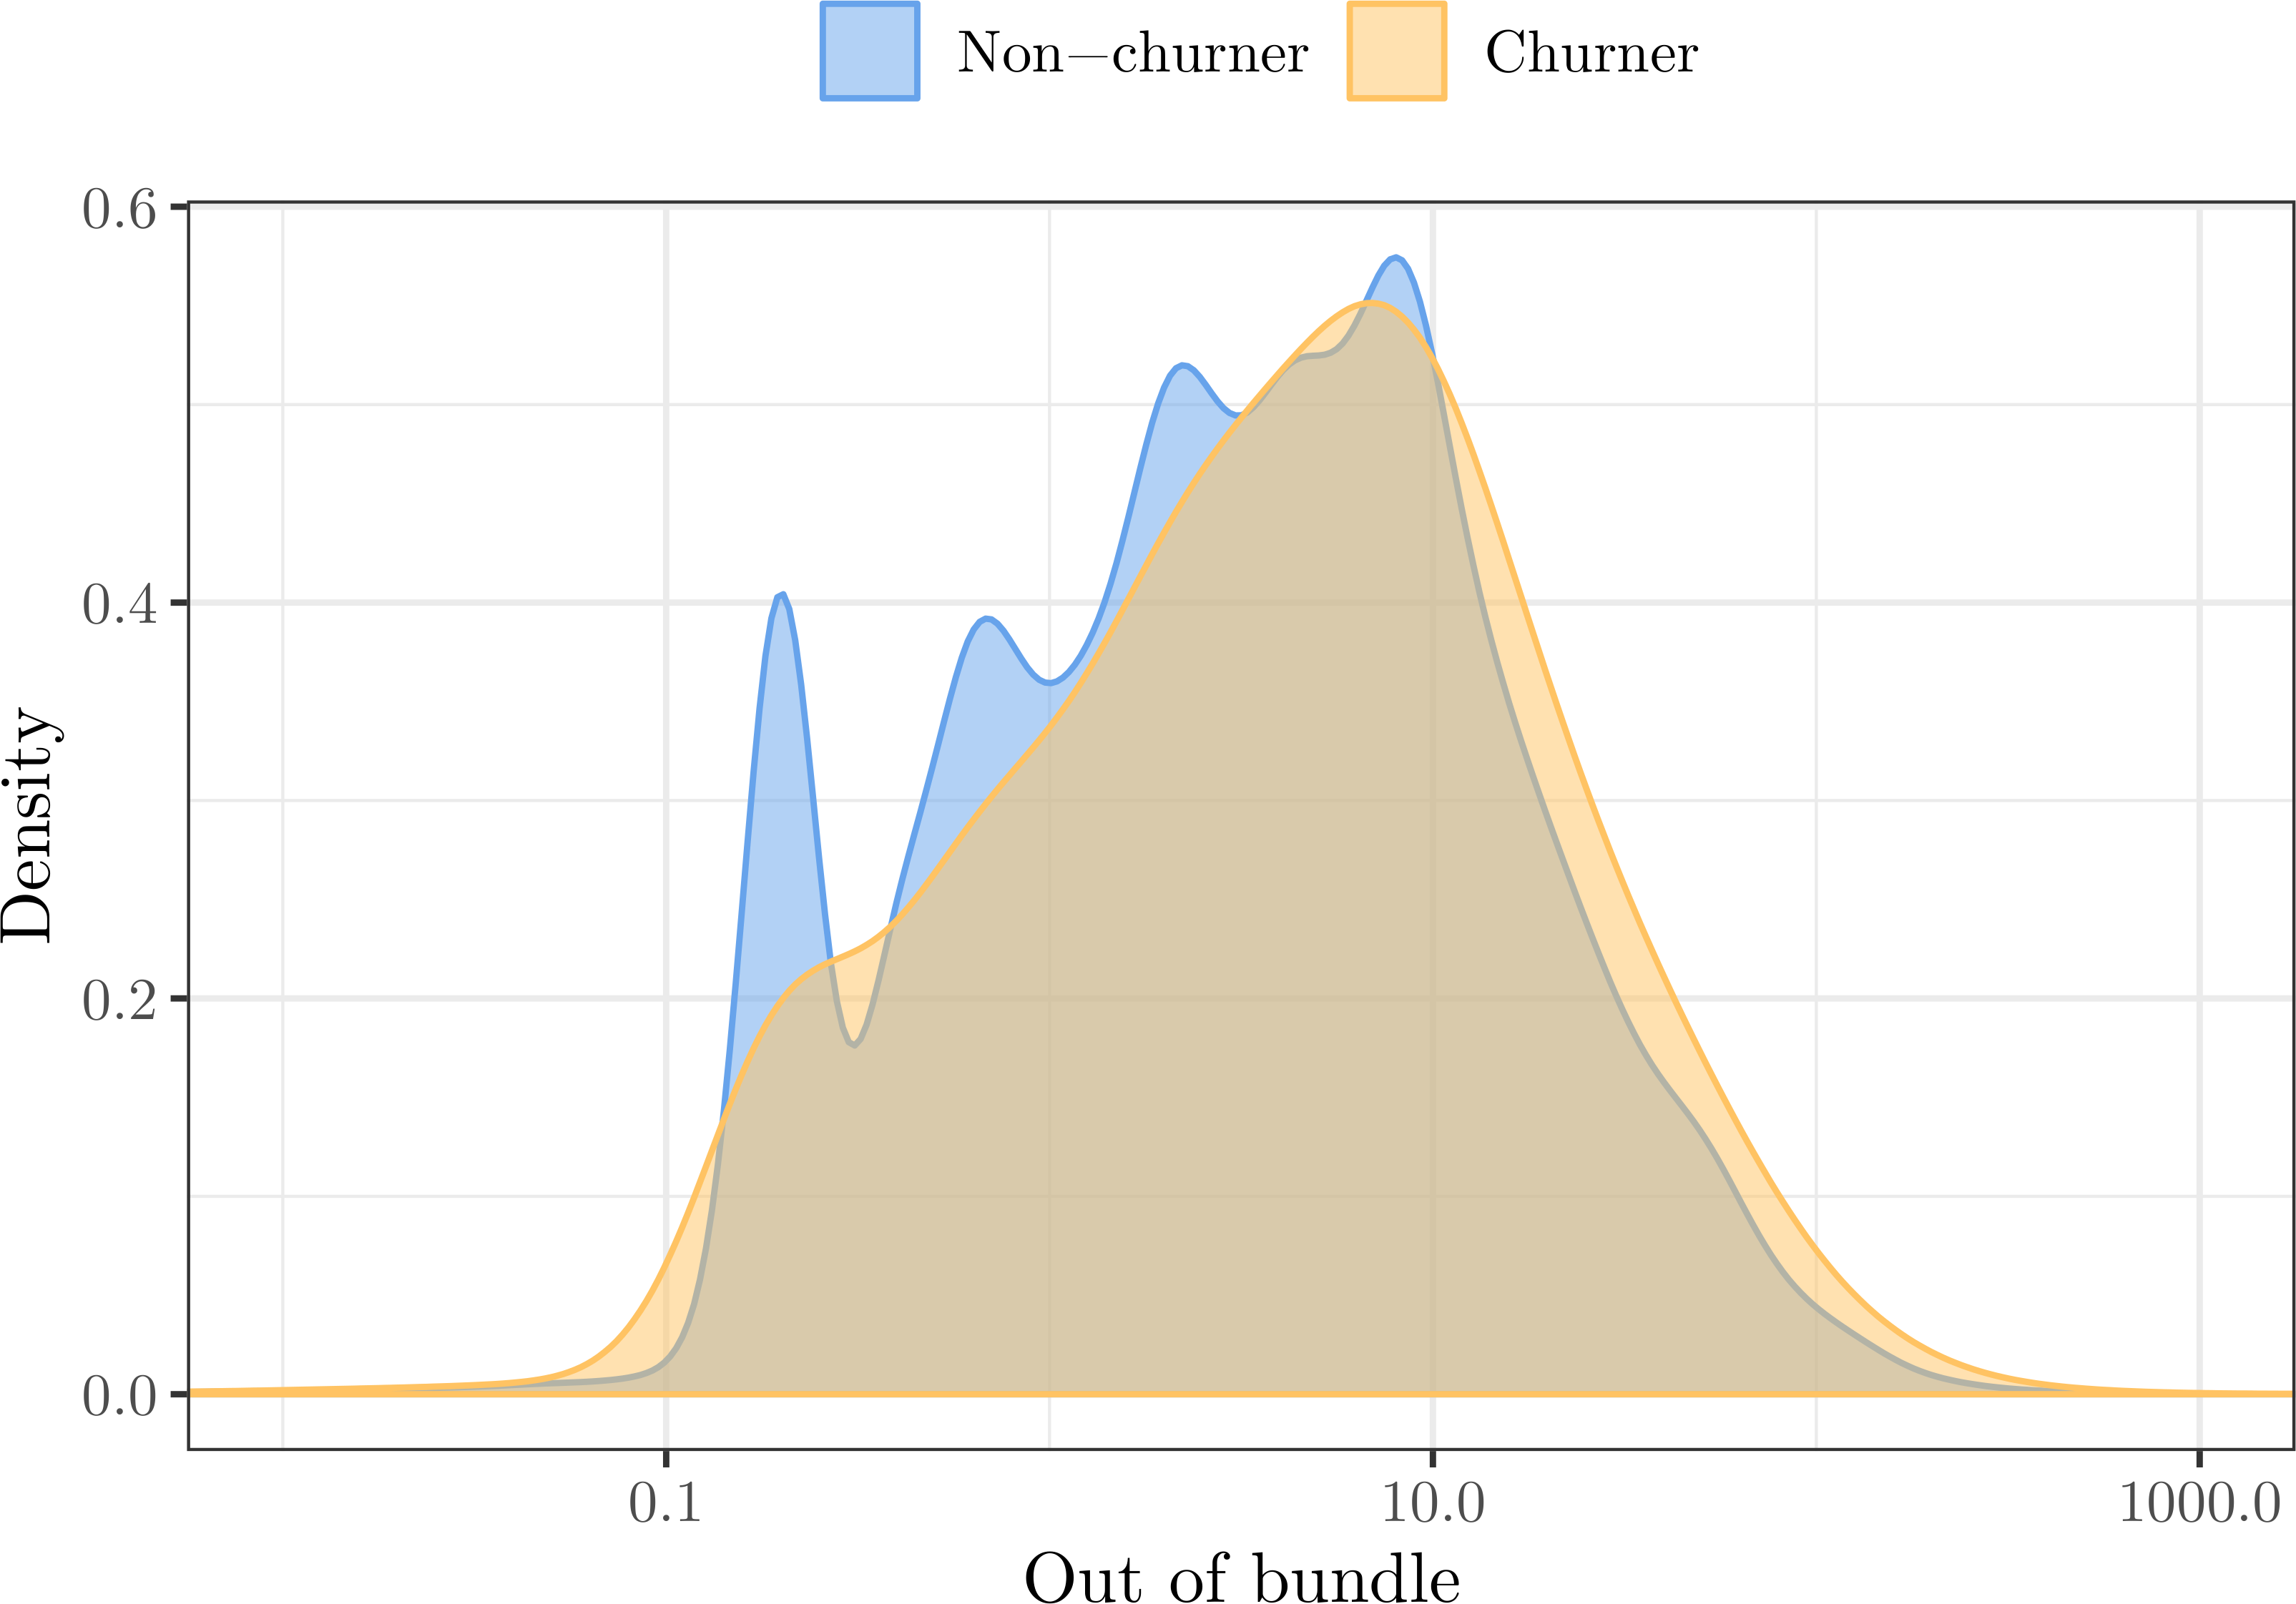
\includegraphics[width=0.9\linewidth]{figures/oob.png}
	\caption{Out-of-bundle amount (extra amount to pay on top of the usual
	invoice), in logarithmic scale.}
	\label{fig:oob}
\end{figure}

The importance of the tenure (the duration of the current subscription) is shown
in figure \ref{fig:tenure}. This graph displays the density of clients as a
function of the tenure. For confidentiality reasons, the scale of the x-axis is
hidden. The curve can be divided into two components: new customers and
long-term customers. One can clearly observe that proportionally more churners
are present in the first component than in the second. This indicates that
long-term clients tend to churn less, whereas new clients are much riskier.

\begin{figure}
    \centering
	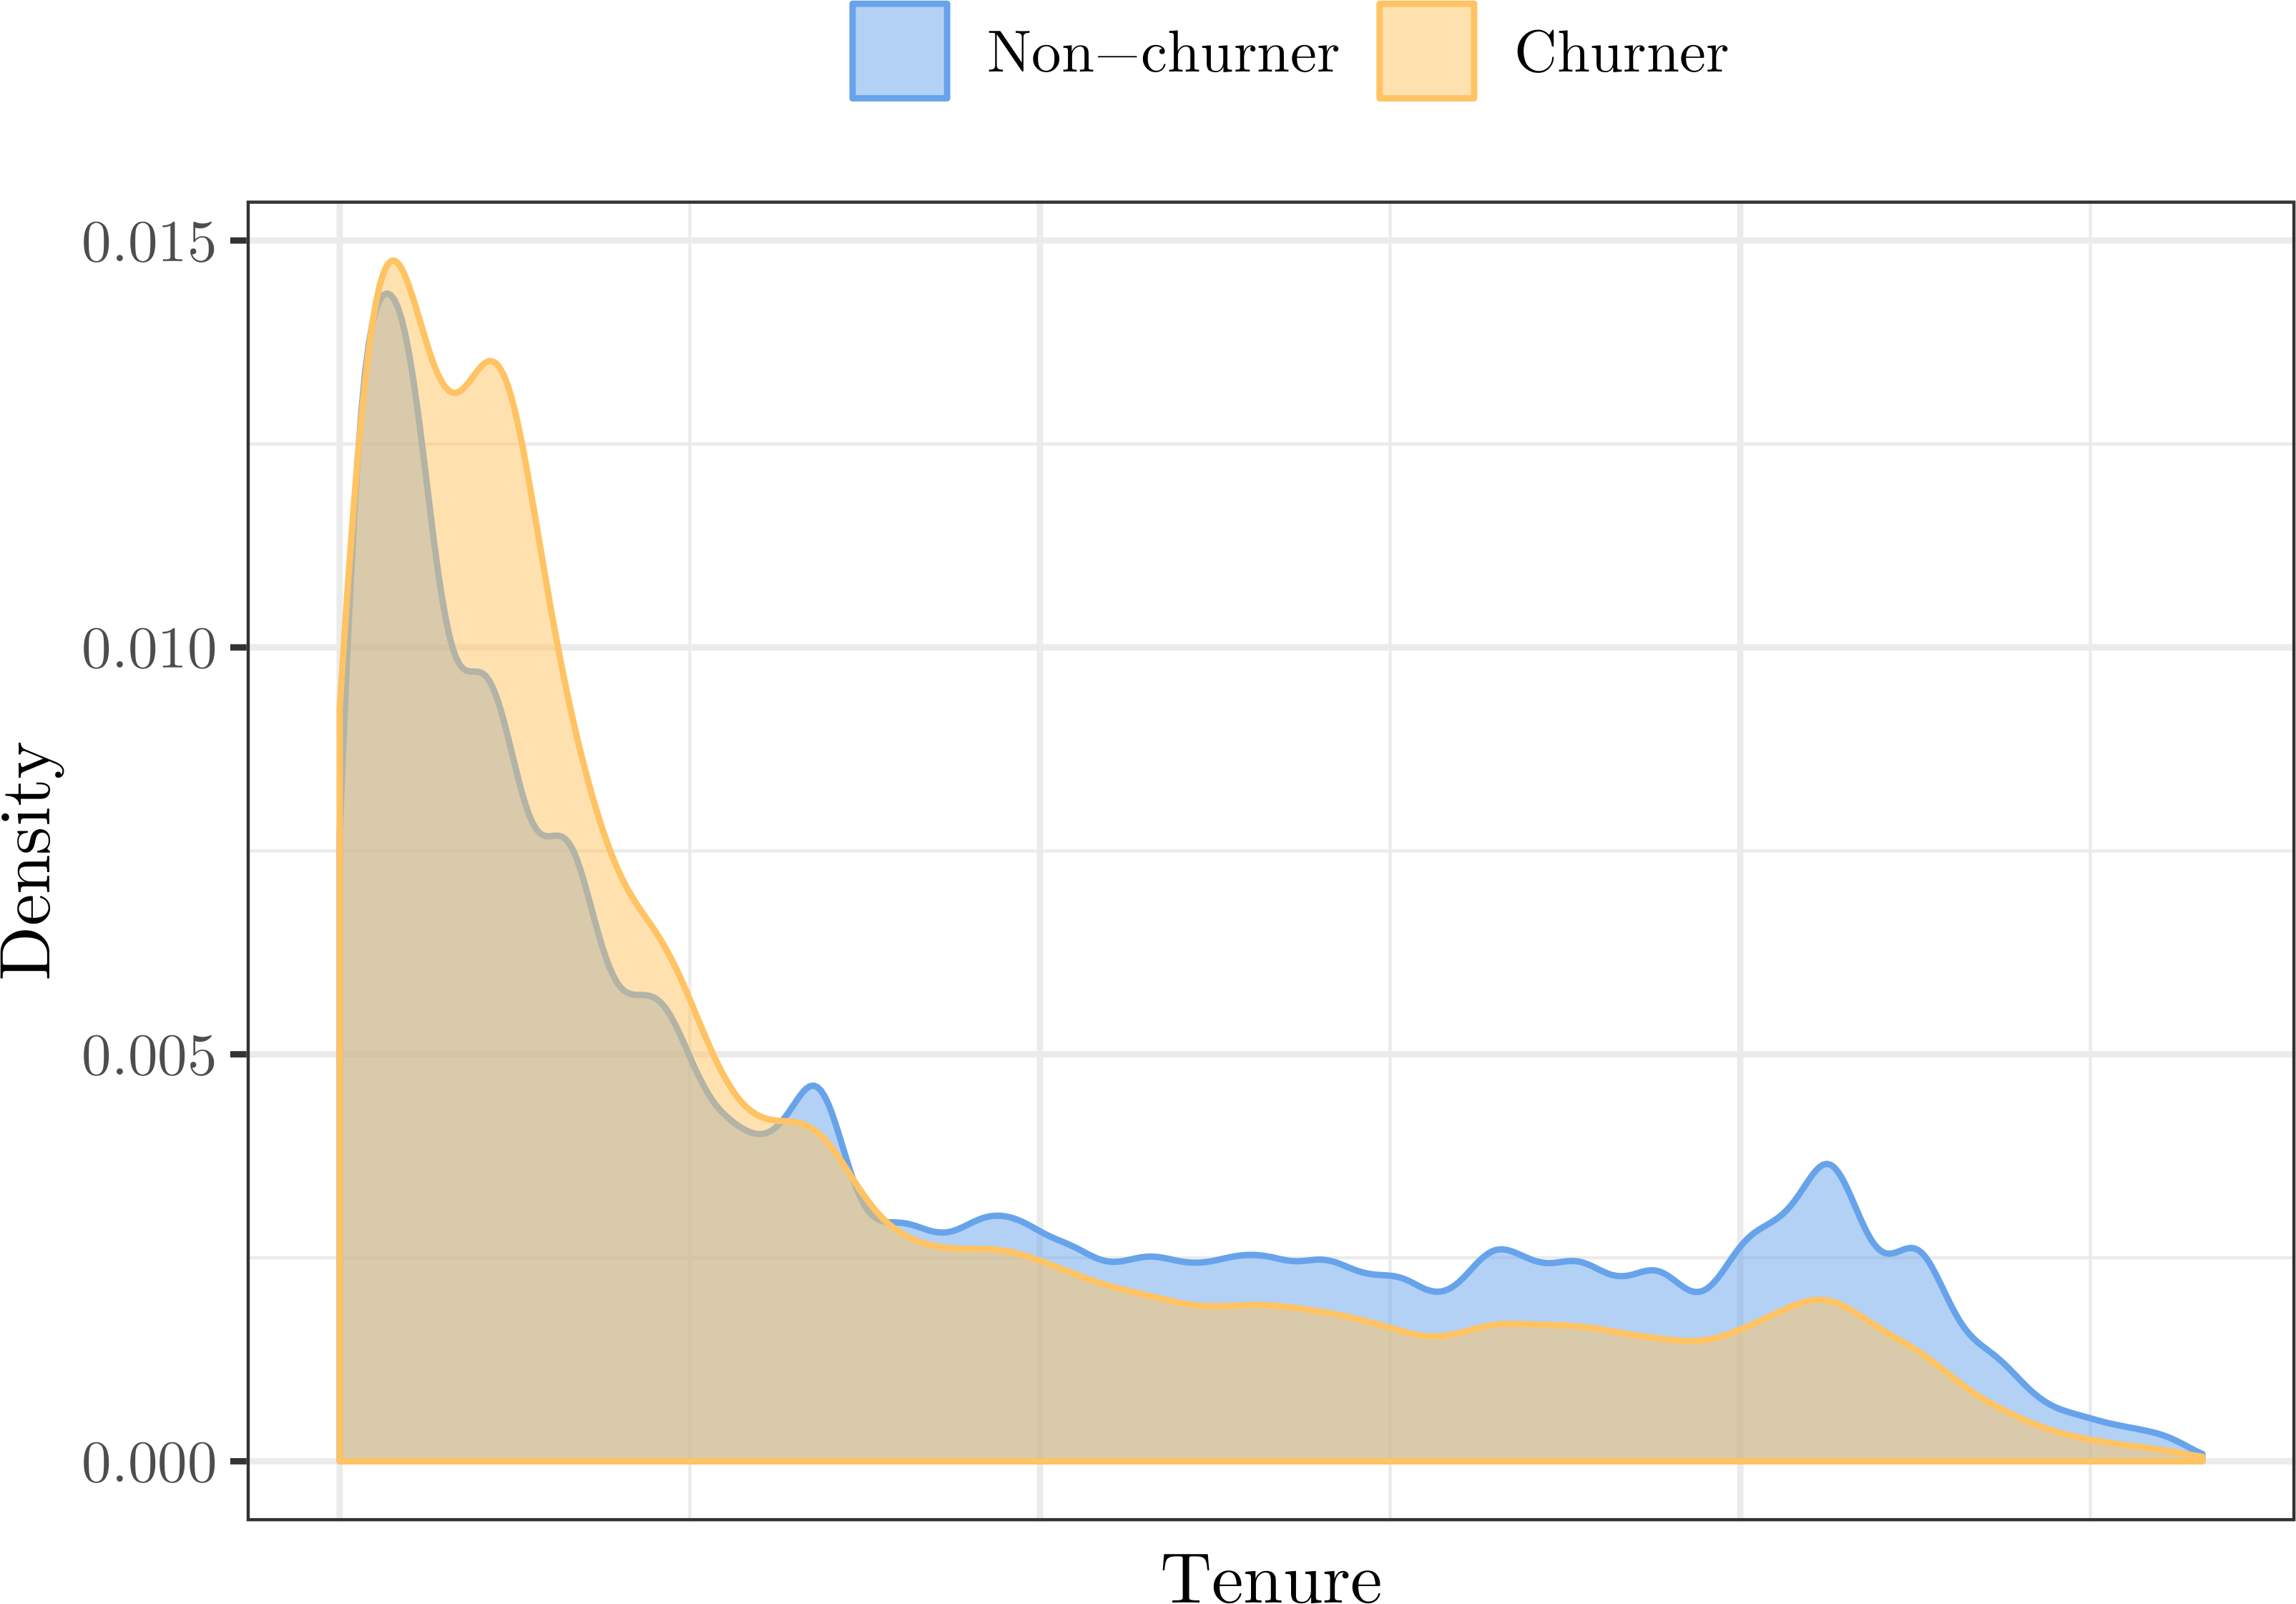
\includegraphics[width=0.9\linewidth]{figures/tenure.png}
	\caption{Tenure (time spent without churning so far) for churners and
	non-churners.}
	\label{fig:tenure}
\end{figure}

Figures \ref{fig:binary} and \ref{fig:categorical} show the distribution of two
discrete categorical variables. The first variable, R14, is a binary flag
related to revenues and is slightly less often true among churners. The second
variable, H8, is a categorical variable related to hardware and takes 8
different values. The churn rate varies moderately depending on the value of
this variable.

\begin{figure}
    \centering
    \begin{minipage}{.45\textwidth}
    	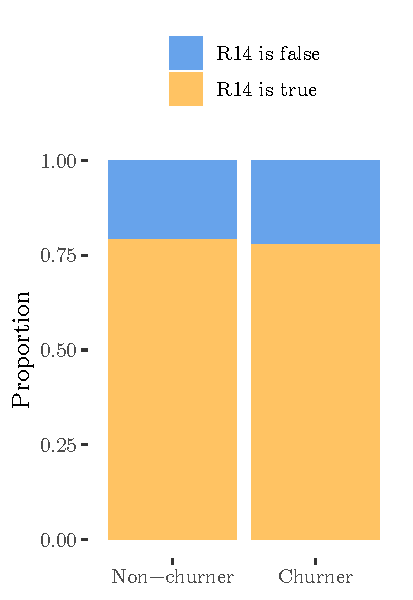
\includegraphics{figures/binary.pdf}
    	\caption{Distribution of a binary variable related to revenues, R14, for
    	churners and non-churners.}
    	\label{fig:binary}
    \end{minipage}
    \hspace{0.05\textwidth}
    \begin{minipage}{.45\textwidth}
    	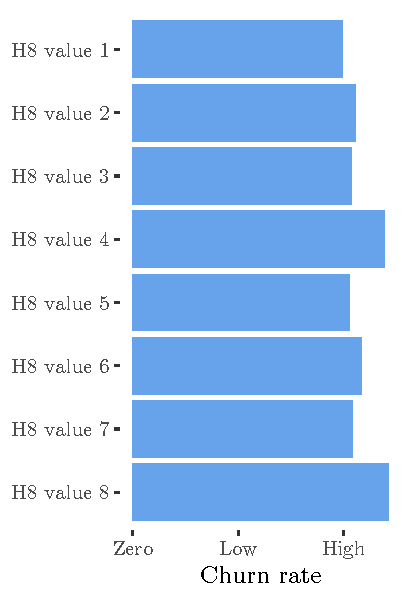
\includegraphics{figures/categorical.pdf}
    	\caption{Distribution of churn rate depending on a categorical variable
    	related to hardware, H8.}
    	\label{fig:categorical}
    \end{minipage}
\end{figure}


We demonstrate the interaction between two categorical variables in figure
\ref{fig:binary_payment_responsible}. The horizontal axis indicates whether a
customer has a cable connection, and the vertical axis denotes the payment
responsible flag. This flag is set to false only when someone else pays the bill
of the customer, such as a parent. Most customers of Orange Belgium do not have
a cable connection, and are responsible for the payment, as indicated by the
radius of the spots. The color of the spots indicates the churn rate, with a
lighter color denoting a higher probability of churn. The area is proportional
to the number of clients in each category. The impact of both binary variables
appears clearly, with a significant difference of churn rate between the two
extrema. Once again, the precise value of churn rate cannot be disclosed.


\begin{figure}
    \centering
	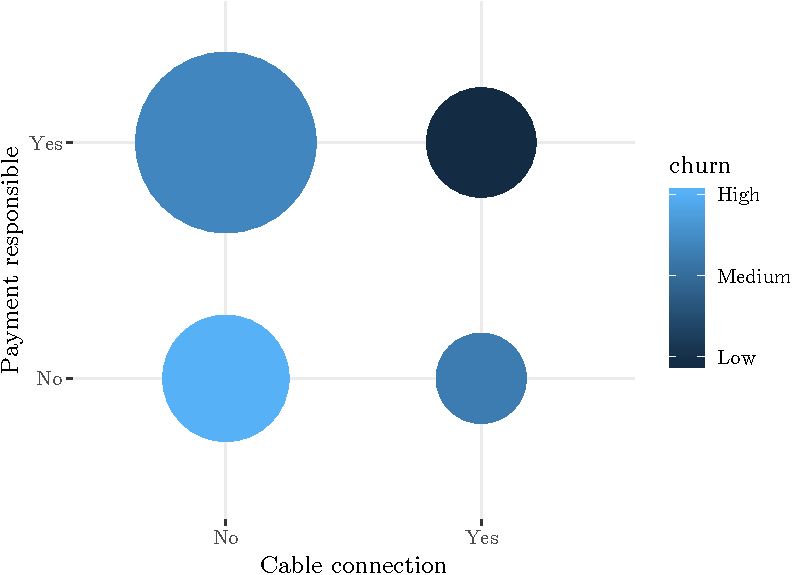
\includegraphics[width=0.9\linewidth]{figures/flagcable_payment_responsible.pdf}
	\caption{Interaction between cable connection and payment responsible. A
	customer is not responsible for payment if someone else (e.g. a parent) pays
	the invoice in her stead. The color of the spots denotes the churn rate,
	whereas its area denotes the number of customers.}
	\label{fig:binary_payment_responsible}
\end{figure}


A principal component analysis (PCA) demonstrates the important overlap between
churners and non-churners (figures \ref{fig:pca_1_2} and \ref{fig:pca_1_2}). The
blue corresponds to non-churners, while the orange and yellow represent
the churners respectively in the validation and the test set. We explain how the
test set and the validation set are partitioned in section
\ref{sec:churn_data_seg}. The ellipses represent the contour lines of
covariance, that is, the set of points at a Mahalanobis distance of 1 from the
mean in each set. The mean of each set is pictured as a dot in the center of the
figure. A large overlap between the population
of churners and non-churners appears clearly. Also, the standard deviation is larger in the
population of churners, reflecting the interpretation that churn is associated
with larger values for the out-of-bundle amount, number of calls, data usage,
etc.

\begin{figure}
    \centering
    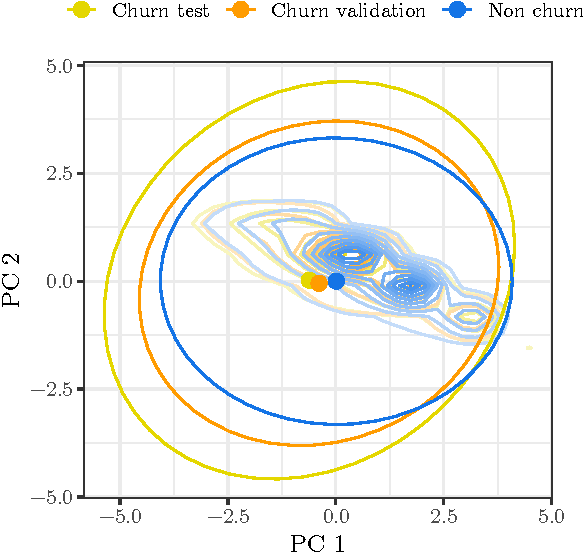
\includegraphics[width=0.63\linewidth]{figures/pca_1_2.pdf}
    \caption{Projection of the dataset onto the first two principal components.
    The ellipses show the set of points at a Mahalanobis distance of 1 from the
    mean of each group, which are represented by a dot.}
    \label{fig:pca_1_2}
\end{figure}

\begin{figure}
    \centering
    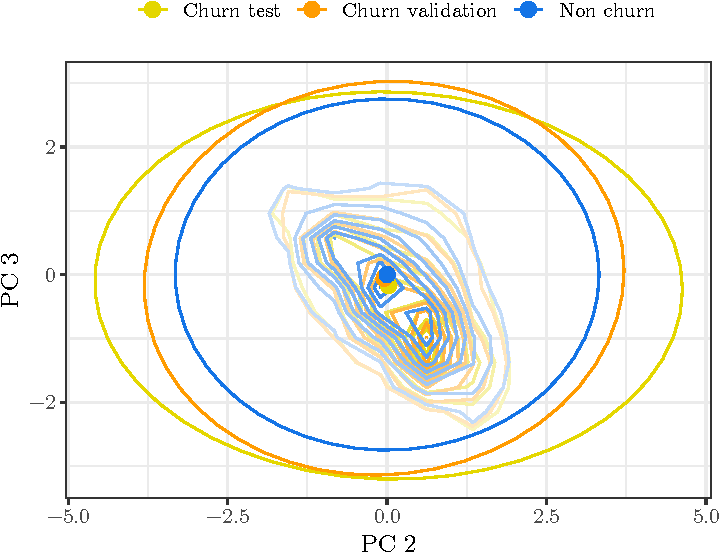
\includegraphics[width=0.8\linewidth]{figures/pca_2_3.pdf}
    \caption{Projection of the dataset onto the second and third principal
    components. The ellipses show the set of points at a Mahalanobis distance of
    1 from the mean of each group, which are represented by a dot.}
    \label{fig:pca_2_3}
\end{figure}

This data analysis demonstrates the high complexity of the churn prediction
problem. No unique variable allows to unambiguously predict churn since there is
a significant overlap between the population of churners and non-churners.
Informative variables such as the tenue (figure \ref{fig:tenure}) or the
out-of-bundle amount (figure \ref{fig:oob}) allow to increase or decrease the
confidence into churn only marginally. A large number of variables must be used
in conjunction in order to achieve decent predictive performances. Moreover, we
have no guarantee that the set of available variables are sufficient, it is
easily conceivable that unknown factors, such as a promotion launched by a
concurrent company, play a significant role.

\section{Data preparation}
\label{sec:data_pre}

The data preparation is of a sequence of steps.

\begin{description}

	\item[Unknown values preprocessing] The original data uses various means to
	specify an unknown categorical value. For example, an unknown previous
	tariff plan is either represented by an empty string, the string
	\texttt{"u"}, the string \texttt{"null"} or a null value. This preprocessing
	step replaces these various encodings by a unique one. Also, missing values
	in continuous variables are either replaced by zero or by the mean of the
	variable, depending on the semantics (e.g. null data usage is replaced by
	zero, whereas missing age is replaced by the average age in the dataset).

	\item[Date encoding] Some fields are represented by a date, such as the last
	contract change, the date of contract activation, or the churn date. These
	fields are converted to the number of days between the first day of the
	month of the dataset entry and the field value. For example, let us consider
	an entry about the activity of a customer in January 2019. Say this entry
	contains a field with the contract activation date, with value \texttt{"20
	December 2018"}. This field is converted to an integer value of 12,
	since there are 12 days between 1st January 2019 and 20 December 2018.

    \item[Clustering of character strings] There are three character string
    variables, representing the current and the previous tariff plan, and the
    manufacturer of the customer's device. These three variables could be
    considered as categorical variables, but the high number of different values
    would make this difficult to implement. We alleviate this difficulty by
    clustering all the different values into a small number of groups. In the
    case of the two tariff plan variables, this corresponds to the different
    tariff plan options (\emph{Hummingbird}, \emph{Koala}, \emph{Eagle}, etc).
    For the device manufacturer, we keep the 7 most common values, and we
    replace all the less frequent values by "Other".

	\item[Difference and ratio columns] For each numerical field representing a
	quantity that can change from month to month (such as the total duration of
	calls, or the mobile data usage), we create 2 additional fields. They
	contain the difference and the ratio of the value of the field with that of
	the same field the previous month. This hopefully gives the model an
	indication of the customer's behavior evolution over the course of the last
	month. 41 variables are suitable for this operation, therefore increasing
	the number of variables up to 155. If no data is available for the previous
	month (such as for the first month of data), the differences are set to 0
	and the ratios are set to 1. In order to reduce computation time, not all
	experiments use these new columns, as discussed in the next section. This
    augmented dataset is named ``SIM only $\Delta$'' thereafter.

	\item[Normalization] The data is normalized to obtain zero mean and unit
	variance. Even though the only models being used are random forests, which
	are not sensitive to linear scaling of its input variables, this step is
	kept in the event that we would have tried another model requiring
	normalization (such as support vector machine or neural networks). This
	preprocessing step is also useful for sensitivity analysis, where we add a
	small value to a variable and observe the difference in the predictions of
	the model. In this case, a normalized dataset allows to use the same
	difference value for all variables.

    \item[Target variable] The last step is to create a binary target variable
    from the churn date. It is defined to be true if and only if the date of
    churn is in the two months following the current data entry. If the churn
    date is in the current month or before, then the entry is discarded, for two
    reasons. Firstly, the information contained in these entries is incomplete.
    Secondly, this data is not relevant for churn prediction, as we wish to
    predict churn at least a few days in advance. It is not interesting to learn
    patterns exhibited by clients that will churn the next day, as there is
    probably no longer any hope of successful retention. If the churn date is
    not given, or if it is more than two months after the month of the data
    entry, the churn variable is set to false. This process is pictured in
    figure \ref{fig:data_separated}. The choice of the time threshold is
    dependent on the business application. A lower threshold focuses on
    short-term churn, whereas a larger threshold enables to predict churn from
    further in the future. Models already in use at Orange Belgium consider a
    time period of two months, we therefore use this value in order to enable
    the comparison of our results with production models.

\end{description}

\begin{figure}
    \centering
	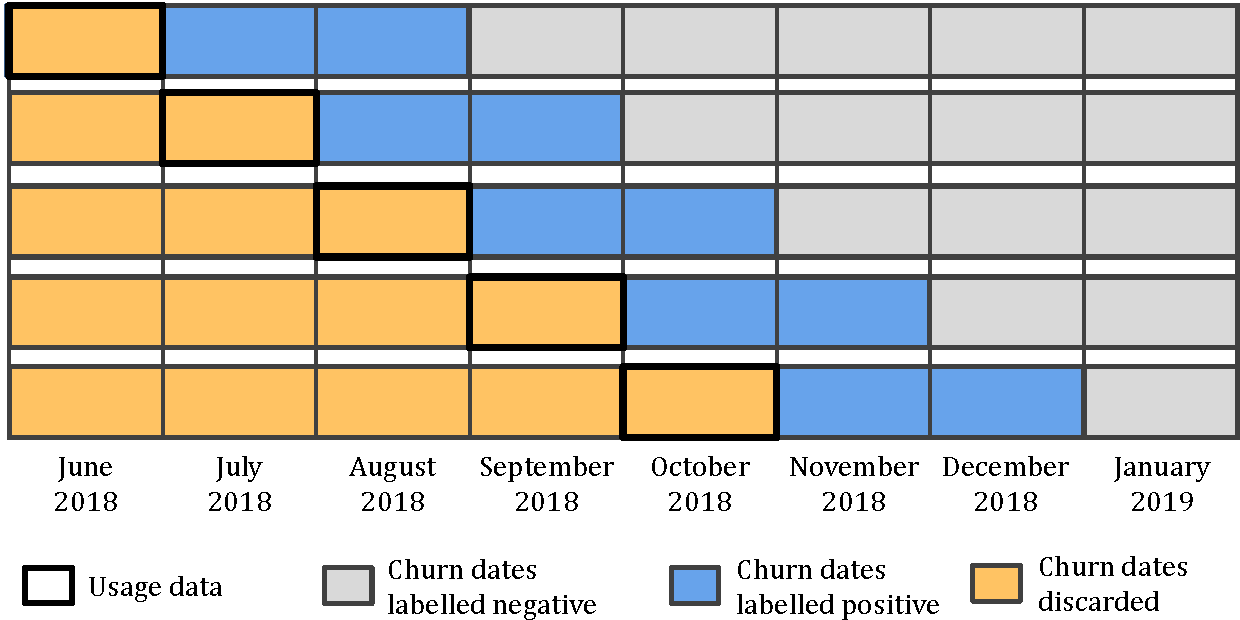
\includegraphics[width=0.9\linewidth]{figures/data_range.pdf}
	\caption{Outline of the target variable assignment. The dataset is separated
	in 5 months and each data entry in each month is labeled as churner if the
	churn date is given and less than two months ahead.}
	\label{fig:data_separated}
\end{figure}

\section{Experiments}
\label{sec:churn_exp}

\subsection{Scope}

The experiments on predictive modeling consist in the training of predictive
models on the data described in the previous sections, and an assessment of
their performance. Three datasets are derived from the output of the
preprocessing step: one containing the loyalty contracts, one containing the SIM
only contracts, and one containing the SIM only contracts with difference and
ratio variables (called SIM only $\Delta$). We evaluate the impact of

\begin{enumerate}
    \item variable selection, based on the feature importance provided by
    trained random forest models;
    \item the addition of difference and ratio variables;
    \item the type of contract (SIM only vs. loyalty).
\end{enumerate}

The high computational cost of the model training on such a large dataset does
not allow to test all the possible configurations of these three parameters. We
limited the number of selected variables to 20, 30 or all variables. Also, we do
not explore the difference variables for loyalty contracts. These
combinations of parameters yield 9 different experiment configurations.


\subsection{Data segmentation}
\label{sec:churn_data_seg}

In each configuration, the corresponding dataset is split into a training and a
test set. The training set comprises the first 4 months of data and the test set
comprises only the last month, as pictured in figure
\ref{fig:experiment_diagram}. Separating by months allows for a potential
concept drift from the training set to the test set (i.e. a change in the
typical behavior exhibited by churners). We perform a $k$-fold cross-validation
on the training set in order to provide an indication of the performance of our
model on the training data. We set $k=3$, as a compromise between statistical
significance and computation time. The difference in prediction accuracy between
the validation set and the test set indicates how much patterns learned on the
training set are still relevant for the next month. This indicates whether
training has to be repeated each month as new data arrives from the customers.
Note that when testing the model on the test set, a new model is trained on the
whole training set.

\begin{figure}
    \centering
	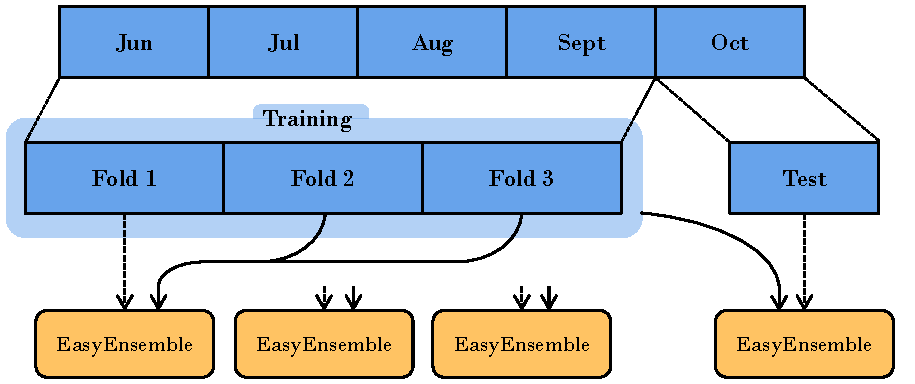
\includegraphics[width=0.9\linewidth]{figures/experiment_diagram.pdf}
	\caption{Outline of the data repartition between training and test set, with
	a 3-fold cross-validation on the training set. Dotted arrows indicate
	testing and solid arrows indicate training. Arrows for two of the three
	validation models are not shown.}
	\label{fig:experiment_diagram}
\end{figure}

\subsection{Class balancing}

In order to counteract the sheer prominence of non-churners in the dataset, we
need to use class balancing. We use the EasyEnsemble algorithm, presented in
section \ref{sec:sota_balancing}. It consists in training different models on
the whole set of positive instances, and on a randomly selected set of negative
instances. The number of negative instances is chosen so that the ratio between
the two classes is even. In all experiments, the EasyEnsemble is set to use 10
random forest models.

\subsection{Evaluation measure}

The performance of the different models is evaluated using three different
measures: the lift curve, the receiver operating characteristic (ROC) curve, and
the precision-recall (PR) curve. While the ROC curve and the PR curve are widely
used in the machine learning literature, the lift curve is of more practical
interest in evaluating churn prediction. Since a customer churn retention
campaign focuses on a limited amount of customers, the lift curve allows
observing the expected performance of the model as the number of customers
included in the campaign varies. From the ROC and PR curves, we derive the area
under the ROC curve (AUROC), the area under the PR curve (AUPRC) and the lift at
different thresholds (1\%, 5\%, and 10\%).

We argue that the most sensible cost evaluation functions are the maximum profit
criterion (MPC) and the expected maximum profit criterion (EMPC)
\parencite{verbeke2012new, verbraken2013novel}. These take into account the
different costs and benefits yielded by a retention campaign and provide the
decision threshold that should be applied to maximize the profit given the
probability distribution output by a prediction algorithm. This process
formalizes the intuition behind the lift criterion that the prediction algorithm
should focus on reducing false positives, since the retention campaign is not
able to reach each and every potential churner. Despite the relevance of this
approach under a profit-centric point of view, we are not able to use this
evaluation measure in our study. This is caused by the necessity to evaluate
different costs and benefits parameters, such as the cost of reaching a
customer, the probability that a customer accepts an incentive, the benefit if
the customer accepts it, etc. The evaluation of these parameters is a
time-consuming process and is outside of the scope of our work.


\subsection{Sensitivity analysis}
\label{sec:churn_sens}

The impact of variables on churn prediction is derived in two different ways.
The first corresponds to the variable importance output by the random forest
models. Each random forest calculates a score for each variable by measuring how
much the prediction accuracy decreases when all the values of this variable are
randomly permuted. The decrease in accuracy is calculated over the out-of-bag
samples in each tree. This permutation cancels out any statistical dependency
between this variable and the target variable, giving an estimate of the
importance of the variable in the trained model. Note that if two variables
share the same information about the target (for example by being highly
correlated), the importance of both of these variables will be less than if only
one were present. This is due to the fact that the two variables are equally
likely to be chosen when splitting nodes in a tree, therefore reducing the
impact of the removing one of the two variables when computing the importance.

This measure of importance allows to understand the predictive power of each
variable but does not indicate the directionality of its impact on the
predictions. We address this issue by constructing, for each variable $X_i$, an
alternate training set identical to the original one, but where a value equal to
one standard deviation $\sigma_{X_i}$ is added to each instance of the variable
$X_i$. A second shifted dataset is also constructed by subtracting instead of
adding the standard deviation. Then, the average predicted probability of churn
is computed for both the original training set and the shifted one, and the
difference between the two average probabilities is taken. This difference
indicates the impact of the variable on the predictions. For example, a
predicted churn probability lower for the training set where a standard
deviation is added to the tenure variable indicates that longer-standing
customers are associated with less churn. Note that we use in this experiment
the normalized dataset so that adding a standard deviation amounts to adding 1
to the instances of the variable.

\section{Results}

\begin{table}
    \centering
    \begin{tabular}{lrrrrrrrrr}
        \toprule
        & \multicolumn{3}{c}{\textbf{SIM only}}
        & \multicolumn{3}{c}{\textbf{SIM only $\Delta$}}
        & \multicolumn{3}{c}{\textbf{Loyalty}} \\
        \cmidrule(l){2-4} \cmidrule(l){5-7} \cmidrule(l){8-10}
        & \textbf{20} & \textbf{30} & \textbf{All} & \textbf{20} & \textbf{30} &
        \textbf{All} & \textbf{20} & \textbf{30} & \textbf{All} \\
        \midrule

        AUROC        & 0.66 & \underline{0.73} & \underline{0.73} & 0.72 &
        \underline{0.73} & 0.69 & 0.74 & \underline{0.76} & \underline{0.76} \\

        AUPRC        & 0.05 & \underline{0.10} & \underline{0.10} &
        \underline{0.10} & \underline{0.10} & 0.08 & 0.15 & \underline{0.19} & 0.18 \\

        Lift at 10\% & 2.25 & 3.34 & 3.41 & 3.27 & \underline{3.42} & 3.03 &
        2.96 & \underline{3.40} & 3.30 \\

        Lift at 5\%  & 2.64 & 4.49 & \underline{4.68} & 4.48 & 4.67 & 4.09 &
        3.51 & \underline{4.22} & 4.02 \\

        Lift at 1\%  & 4.29 & 9.20 & 9.53 & \underline{10.09} & 9.95 & 7.67 &
        4.66 & \underline{6.65} & 6.16 \\
        \bottomrule
    \end{tabular}
    \caption{Summary of the results of prediction experiments on the test set.
    Highest values for each type of contract and for each evaluation measure are
    underlined for the test set.}
    \label{tab:results}
\end{table}

This section shows the results of the predictive experiments. Figures
\ref{fig:lift_simo} to \ref{fig:pr_loy} are performance curves for the three
different datasets. Each plot contains a curve for both validation and test
sets, and for the configurations where we select 20, 30 or all of the variables.
This amounts to a total of 6 curves per plot. As explained in section
\ref{sec:churn_exp}, the validation is done on the 4 first months of data,
whereas the test set corresponds to the last month. Figures \ref{fig:lift_simo}
to \ref{fig:lift_loy} show the lift curves, figures \ref{fig:roc_simo} to
\ref{fig:roc_loy} show the ROC curves, and figures \ref{fig:pr_simo} to
\ref{fig:pr_loy} show the precision-recall curves. A summary of the results is
given in table \ref{tab:results}. The lift at different thresholds, the area
under the ROC curve, and the area under the precision-recall curves are reported
for the test set. Table \ref{tab:results_valid} provides the same information
for the predictions on the validation set. The impact of the different
experimental parameters on predictive performance is discussed in the next
sections.

In this section, numerical scores associated with variables are displayed as
horizontal bar plots. The colors of the bars correspond to the
categories of variables presented in section \ref{sec:churn_data}:

\begin{itemize}
    \item[\color{themeyellow}$\blacksquare$] \setulcolor{themeyellow}\ul{Subscription}
    \item[\color{themeblue}$\blacksquare$] \setulcolor{themeblue}\ul{Calls and messages}
    \item[\color{darkerblue}$\blacksquare$] \setulcolor{darkerblue}\ul{Mobile data usage}
    \item[\color{themepurple}$\blacksquare$] \setulcolor{themepurple}\ul{Revenue}
    \item[\color{darkerorange}$\blacksquare$] \setulcolor{darkerorange}\ul{Customer hardware}
    \item[\color{themeorange}$\blacksquare$] \setulcolor{themeorange}\ul{Socio-demographic}
\end{itemize}

\begin{figure}
    \centering
    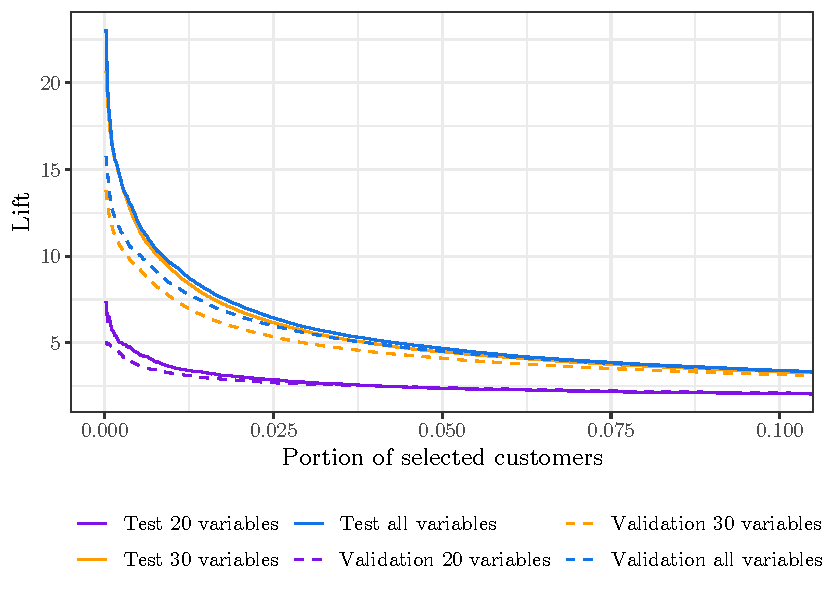
\includegraphics[width=0.9\linewidth]{figures/lift_simo.pdf}
    \caption{Lift curve for SIM only}
    \label{fig:lift_simo}
\end{figure}

\begin{figure}
    \centering
    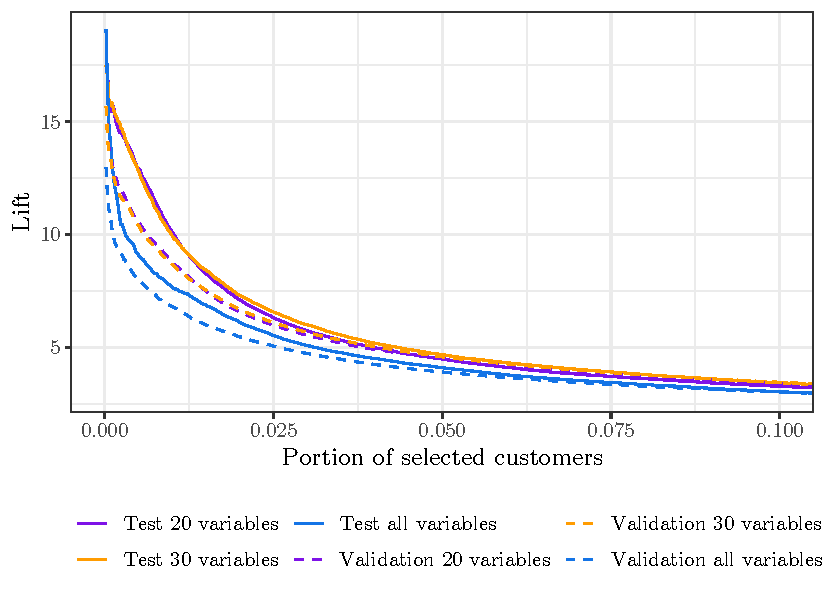
\includegraphics[width=0.9\linewidth]{figures/lift_simo_diff.pdf}
    \caption{Lift curve for SIM only with difference and ratio variables}
    \label{fig:lift_simo_diff}
\end{figure}

\begin{figure}
    \centering
    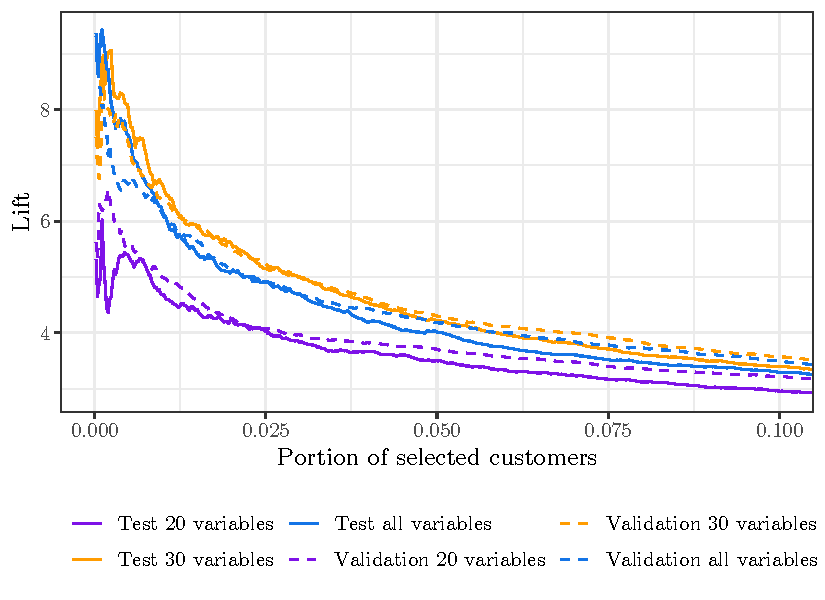
\includegraphics[width=0.9\linewidth]{figures/lift_loy.pdf}
    \caption{Lift curve for loyalty}
    \label{fig:lift_loy}
\end{figure}

\subsection{Number of variables}

The number of variables has an influence on the prediction accuracy, and this
impact depends on the dataset under consideration. Recall that in each
configuration, the selected variables are chosen according to the variable
importance given by the random forests trained on the whole training set. In the
case of the SIM only dataset (figures \ref{fig:lift_simo}, \ref{fig:roc_simo}
and \ref{fig:pr_simo}), selecting only 20 variables decreases drastically the
performance. Selecting 30 variables achieves performances almost as good as
selecting the whole set of 73 variables.

\begin{figure}
    \centering
    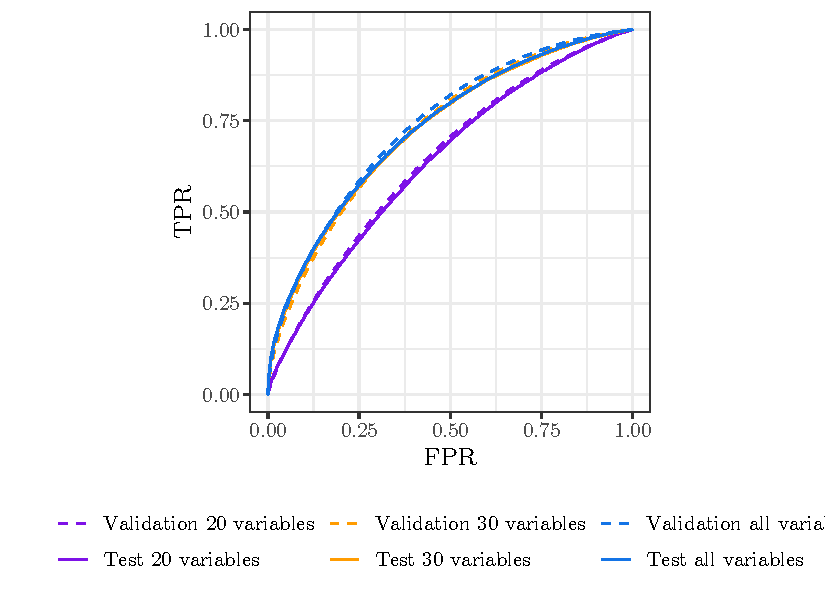
\includegraphics[width=0.9\linewidth]{figures/roc_simo.pdf}
    \caption{ROC curve for SIM only.}
    \label{fig:roc_simo}
\end{figure}

For the SIM only $\Delta$ dataset, a lower number of variables is beneficial for
performance. As shown in figures \ref{fig:lift_simo_diff},
\ref{fig:roc_simo_diff} and \ref{fig:pr_simo_diff}, selecting all variables
appears to be detrimental to the accuracy, whereas choosing between 20 or 30
variables does not make a significant difference. This might be caused by the
additional variables that add more noise than useful information for the random
forests. It is interesting to note that selecting the top 20 variables when
considering the SIM only $\Delta$ dataset provides much better accuracy than
selecting the top 20 variables in the original dataset. As shown in figure
\ref{fig:var_imp_simo_diff_decrease_accuracy}, the 20 most important variables
in the SIM only $\Delta$ dataset do not even include any difference or ratio
variable. The difference between the top 20 most important variables is as
follow:

\begin{itemize}
    \item SIM only $\Delta$ includes the number of contracts, the age, and a
    variable on data usage, whereas SIM only does not;
    \item SIM only includes the device manufacturer, the previous tariff plan,
    and two other variables on data usage, whereas SIM only $\Delta$ does not.
\end{itemize}

\begin{figure}
    \centering
    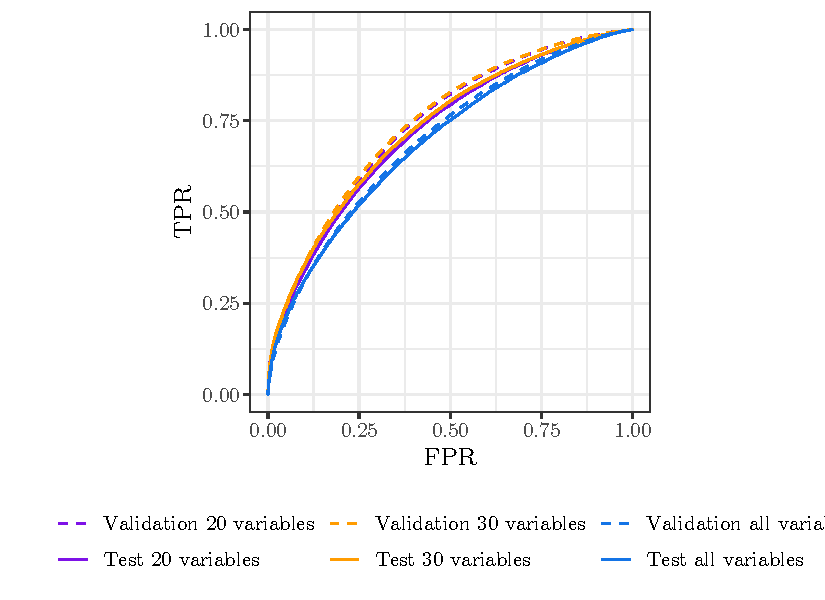
\includegraphics[width=0.9\linewidth]{figures/roc_simo_diff.pdf}
    \caption{ROC curves for SIM only with difference and ratio variables.}
    \label{fig:roc_simo_diff}
\end{figure}

The large difference in accuracy between these two configurations must be caused
by this difference in the selected variables, since all other variables and all
other experiment parameters are identical.

When considering the loyalty dataset, selecting 30 variables instead of the
whole set of 73 variables is marginally beneficial on low thresholds (less than
0.1). On the overall space of thresholds, the difference is not significant, as
indicated in table \ref{tab:results} with the AUROC and the AUPRC. However,
selecting only 20 variables is clearly detrimental.

\begin{figure}
    \centering
    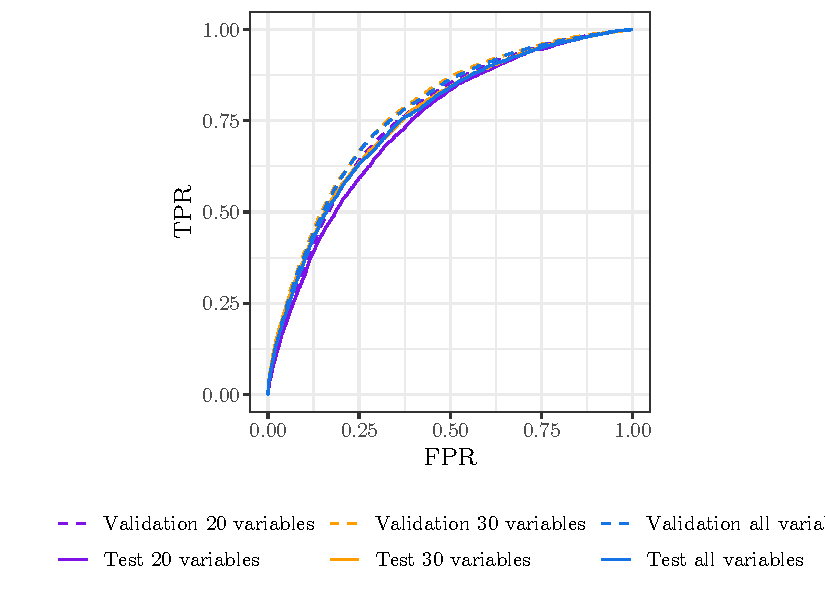
\includegraphics[width=0.9\linewidth]{figures/roc_loy.pdf}
    \caption{ROC curves for loyalty.}
    \label{fig:roc_loy}
\end{figure}

\subsection{Difference and ratio variables}

The difference and ratio variables do not have a positive impact on performance.
Indeed, the best performance achieved on the SIM only $\Delta$ dataset are
obtained by limiting the number of variables to 20 or 30. The variables being
selected in these cases do not include any of the difference and ratio
variables. If all variables are used, the performance of the random forests
decreases significantly, as shown in figures \ref{fig:lift_simo_diff},
\ref{fig:roc_simo_diff}, \ref{fig:pr_simo_diff}, and table \ref{tab:results}.
Moreover, the memory usage of this dataset is much higher than that of the
original dataset, thus complicating the training process.

\begin{figure}
    \centering
    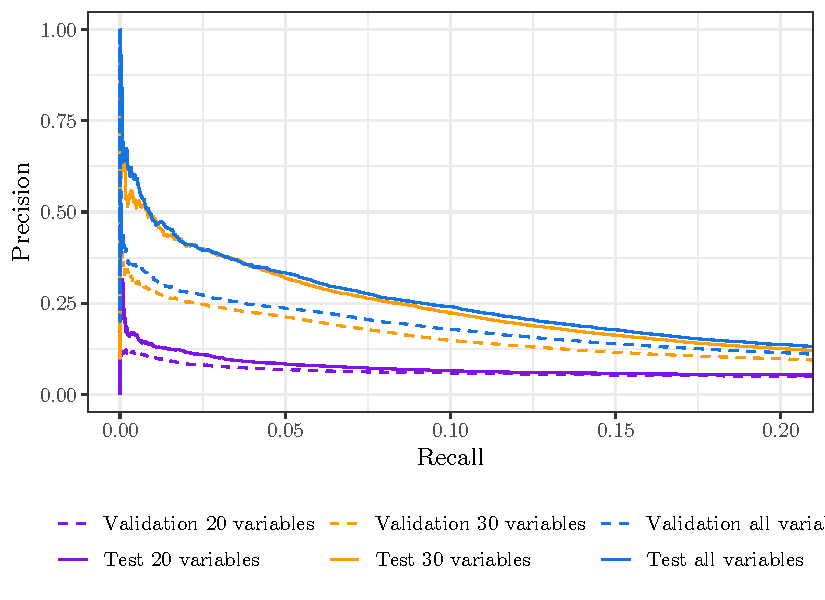
\includegraphics[width=0.9\linewidth]{figures/pr_simo.pdf}
    \caption{Precision-recall curves for SIM only.}
    \label{fig:pr_simo}
\end{figure}

\begin{figure}
    \centering
    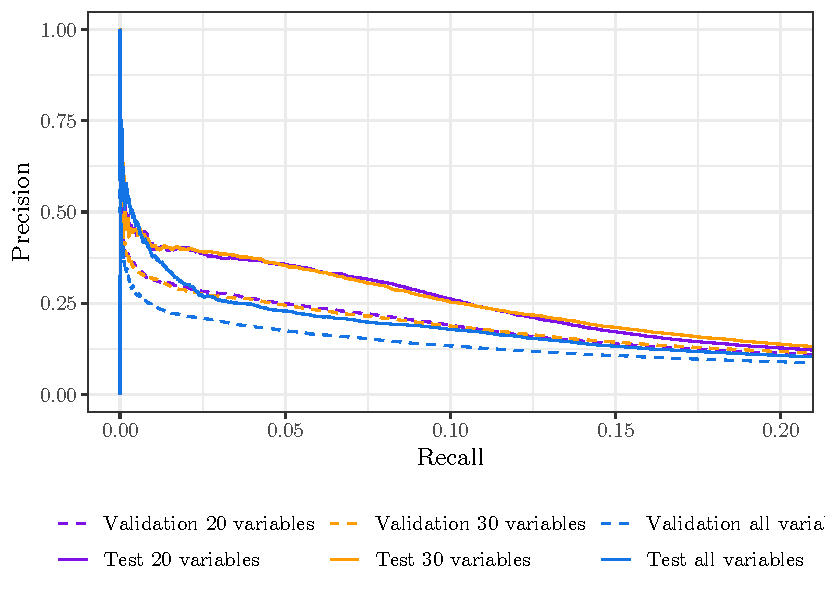
\includegraphics[width=0.9\linewidth]{figures/pr_simo_diff.pdf}
    \caption{Precision-recall curves for SIM only with difference and ratio
    variables.}
    \label{fig:pr_simo_diff}
\end{figure}

\begin{figure}
    \centering
    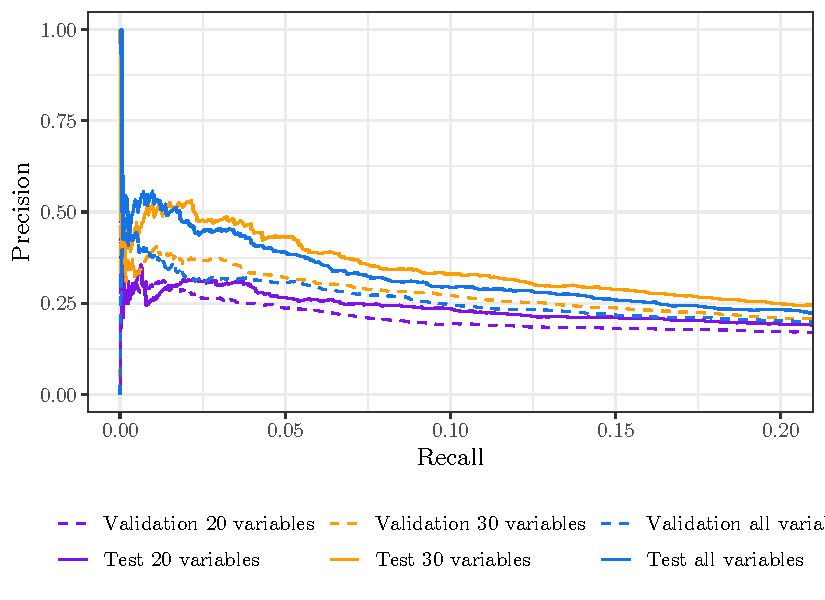
\includegraphics[width=0.9\linewidth]{figures/pr_loy.pdf}
    \caption{Precision-recall curves for loyalty.}
    \label{fig:pr_loy}
\end{figure}

\subsection{Generalization performances}

The generalization abilities of the trained models are evaluated by comparing the
accuracy on the validation set and on the test set. On the lift curves and on
the precision-recall curves, it appears that for all configurations, the
performance on the test set is better than on the validation set. Bear in mind
that on these curves, only a small fraction of the threshold space is
represented, whereas the ROC curves show all possible decision thresholds. This
observation implies that customers with a very high probability of churn are
proportionally more numerous in the test set than in the validation set. It is
illustrated in figures \ref{fig:pca_1_2} and \ref{fig:pca_2_3}, where the
ellipse of covariance of the test set is larger than that of the validation set.
This suggests that, in the test set, there are more churners with very high
values for variables having a large standard deviation. This probably
corresponds to the bill shock effect discussed in section \ref{sec:churn_data}:
a large ``out of bundle'' amount, caused by large data consumption, increases
the probability of churn. In this case, the bill shock is more pronounced in
the test set, explaining the improvement in predictions.

The performance measures on the validation set are summarized in table
\ref{tab:results_valid}. When we compare the lift at low thresholds in table
\ref{tab:results}, it is clear that the model manifests worse performance on the
validation set than on the test set. However, it is not the case for the AUROC
and the AUPRC, which take into account the whole space of decision threshold,
and not only the riskiest customers. We can conclude that our model has been
trained on a training set where the overlap between churners and non-churners is
more important than on the test set. The model thus generalizes well, and even
perform better on unseen data in our case due to a lucky domain shift.

\begin{table}
    \centering
    \begin{tabular}{lrrrrrrrrr}
        \toprule
        & \multicolumn{3}{c}{\textbf{SIM only}}
        & \multicolumn{3}{c}{\textbf{SIM only $\Delta$}}
        & \multicolumn{3}{c}{\textbf{Loyalty}} \\
        \cmidrule(l){2-4} \cmidrule(l){5-7} \cmidrule(l){8-10}
        & \textbf{20} & \textbf{30} & \textbf{All} & \textbf{20} & \textbf{30} &
        \textbf{All} & \textbf{20} & \textbf{30} & \textbf{All} \\
        \midrule
        AUROC & 0.64 & 0.73 & 0.74 & 0.74 & 0.74 & 0.70 & 0.76 & 0.78 & 0.77 \\
        AUPRC & 0.04 & 0.08 & 0.08 & 0.09 & 0.09 & 0.07 & 0.13 & 0.16 & 0.15 \\
        Lift at 10\%  & 2.10 & 3.16 & 3.39 & 3.39 & 3.44 & 3.01 & 3.22 & 3.57 & 3.50 \\
        Lift at  5\%  & 2.41 & 4.11 & 4.52 & 4.49 & 4.57 & 3.90 & 3.71 & 4.30 & 4.18 \\
        Lift at  1\%  & 3.24 & 7.58 & 8.36 & 8.80 & 8.67 & 6.79 & 5.00 & 6.37 & 6.11 \\
        \bottomrule
    \end{tabular}
    \caption{Summary of the results of prediction experiments on the validation
    set.}
    \label{tab:results_valid}
\end{table}

\subsection{Type of contract}

As indicated in table \ref{tab:results}, the models trained on loyalty perform
slightly worse than that of the SIM only datasets on small thresholds, but better
on larger thresholds. The AUROC is equal to 0.76 for loyalty, whereas the best
performing configuration for SIM only achieves an AUROC of 0.73. The AUPRC is
almost double, and this can be seen in figure \ref{fig:pr_loy}. The
precision is similar to that of the SIM only for low recall, but decreases much
more slowly. It is still at approximately 0.25 when the recall is 0.2, whereas,
in the SIM only PR curves, the precision is already at 0.12 at this threshold.

Recall that there are fewer loyalty customers than SIM only, less confidence can
thus be given to the statistical results for loyalty, especially at low
thresholds. According to these results, the models trained on the loyalty
customers are slightly less efficient on small thresholds, but this is made up
for on larger thresholds. The increase in performance is probably due to the
more obvious churn patterns exhibited by loyalty customers. Indeed, most of the
churn in this population is due to the end of the mandatory period of the
subscription. This is reflected in figure
\ref{fig:var_imp_loy_decrease_accuracy}, where time-related variables are
prominent in variable importance. Given that we know when the mandatory part of
the customer's contract ends, the confidence of the model in the probability of
churn is increased compared to the SIM only case.

\subsection{Sensitivity analysis}

The results of sensitivity analysis are shown in figures
\ref{fig:var_imp_simo_decrease_accuracy} to \ref{fig:offset_1m}. Figures
\ref{fig:var_imp_simo_decrease_accuracy} to
\ref{fig:var_imp_loy_decrease_accuracy} show the variable importance given by
the random forest models. There is one plot per dataset, and in each plot the
importance of each variable is averaged over the 10 models underlying the Easy
Ensemble meta-model. As discussed in the previous section, the most important
variables for the SIM only and the SIM only $\Delta$ datasets are almost
identical. They consist in a mix of socio-demographic variables (e.g. the
province), information about the tenure and the tariff plan of the customer, and
aggregate variables related to phone calls. The difference and ratio variables
are ranked fairly low for SIM only $\Delta$, the first one having a rank of 40
(not shown in figure \ref{fig:var_imp_simo_diff_decrease_accuracy}). On the
other hand, the selected variables for the loyalty dataset (figure
\ref{fig:var_imp_loy_decrease_accuracy}) are quite different. The tenure (first
and third variables) and other time-related variables on the subscription are
all important variables. Information relative to the type and time of
subscription is therefore important for predicting churn in loyalty contracts.
This is illustrated by the yellow color dominating the graph. Also, the age is
more important than for the SIM only dataset, as well as the variables U1, U2,
and U3, corresponding to data usage. This is consistent with an interpretation
of a younger and fickler customer base, consuming more data and more prone to
churn.

\begin{figure}
    \centering
    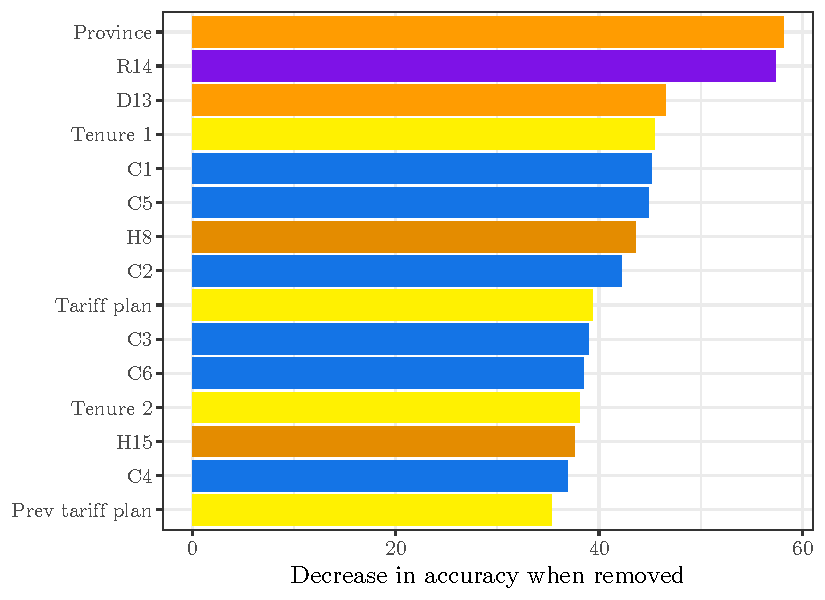
\includegraphics[width=0.9\linewidth]{figures/var_imp_simo_decrease_accuracy.pdf}
    \caption{Mean decrease in accuracy when a feature is removed for SIM only.}
    \label{fig:var_imp_simo_decrease_accuracy}
\end{figure}


Figures \ref{fig:offset_1p} and \ref{fig:offset_1m} display the shift in
predicted churn probability when a variable is offset by one standard deviation.
Figure \ref{fig:offset_1p} corresponds to an increase in the value of each
variable, whereas figure \ref{fig:offset_1m} corresponds to a decrease. The
tenure and the number of contracts have a symmetric effect: an observed increase
in their value reduces the probability of churn, and conversely. For the tenure,
this corresponds to the intuition that a newer customer is more prone to churn.
The number of contracts is a marker of commitment of a customer to Orange, and
the presence of this variable in both figures \ref{fig:offset_1p} and
\ref{fig:offset_1m} expresses that it has also a monotonic relation to churn
probability.


\begin{figure}
    \centering
    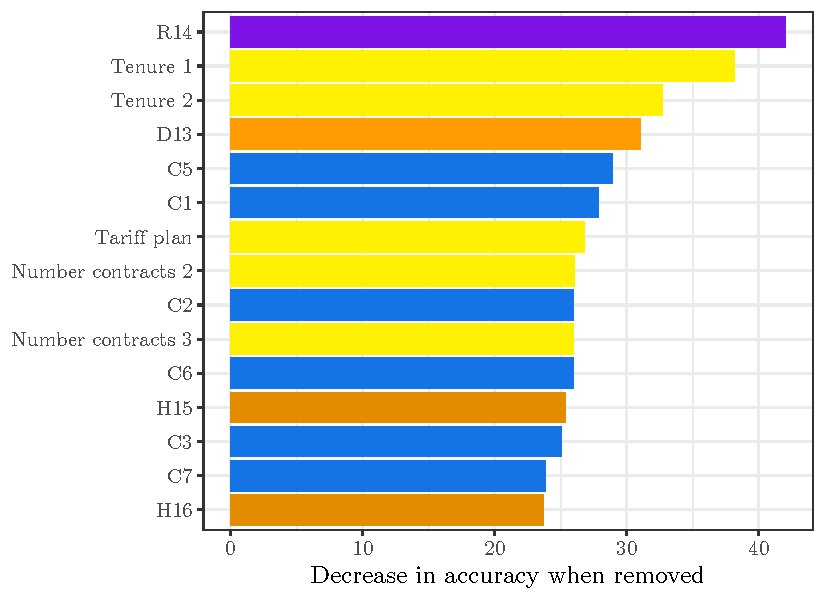
\includegraphics[width=0.9\linewidth]{figures/var_imp_simo_diff_decrease_accuracy.pdf}
    \caption{Mean decrease in accuracy when a feature is removed for SIM only
    with difference and ratio variables.}
    \label{fig:var_imp_simo_diff_decrease_accuracy}
\end{figure}


On the other hand, all other variables in this sensitivity analysis display a
non-linear relationship to predicted churn probability. This is remarkably
illustrated by the prominence of variables related to revenues in figure
\ref{fig:offset_1p}, colored in purple. These variables increase the predicted
probability of churn when they are increased, as expected by the bill shock
effect. However, they are absent from figure \ref{fig:offset_1m}, indicating
that a reduced bill is not associated with a reduced churn. It is worth mentioning
that the age is associated in both graphs with an increased risk of churn.
Consequently, any age far from the average age is associated with an increased
risk of churn.


\begin{figure}
    \centering
    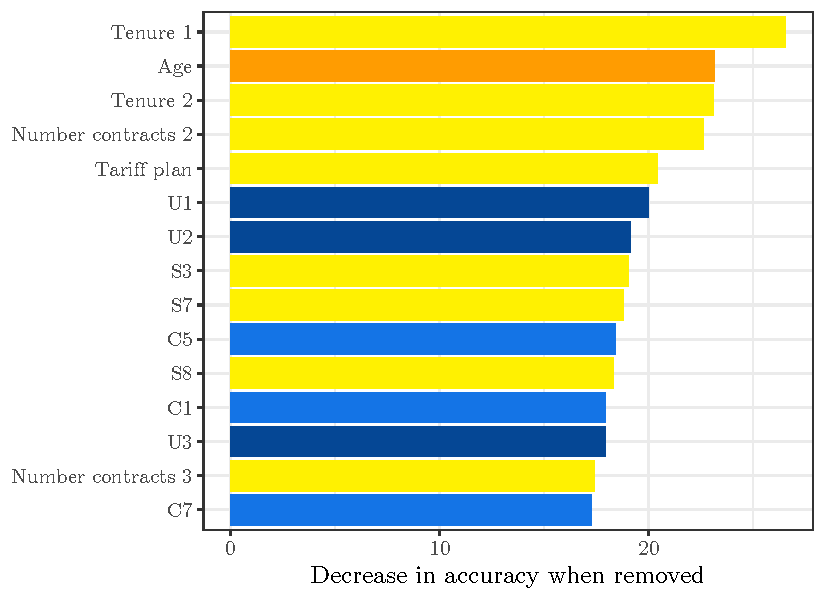
\includegraphics[width=0.9\linewidth]{figures/var_imp_loy_decrease_accuracy.pdf}
    \caption{Mean decrease in accuracy when a feature is removed for loyalty.}
    \label{fig:var_imp_loy_decrease_accuracy}
\end{figure}

Bear in mind that this analysis is solely indicating statistical associations
between the values of different variables and the predicted probability of
churn. It is by no means an indication of causality. For example, the number of
contracts is inversely associated with the risk of churn. It is tempting to
conclude that selling new contracts to customers will therefore reduce their
risk of stopping their subscription. Nevertheless, the analysis does not confirm
this hypothesis: it might be the case that a satisfied customer is typically not
likely not churn and is also more prone to buying new services. In this case,
the churn and the number of contracts have a common cause (customer
satisfaction), and manipulating the number of contracts will not modify the risk
of churn. Also, the magnitudes of the difference in churn rates should not be
considered as realistic, meaningful values. We added a standard deviation to
each variable, regardless of whether a standard deviation makes sense for each
variable. For example, the number of contracts is typically not distributed
according to a Gaussian distribution, since it takes as value only small
positive integers. We can expect most of the decision trees composing our model
to choose a split point close to 1 for this variable, in order to categorize
clients as either having 1 contract or more. Adding a standard deviation to the
variable would change the path of each sample in these trees. This explains the
disproportionate 15\% of difference in churn rate in figure \ref{fig:offset_1m}.

\begin{figure}
    \centering
    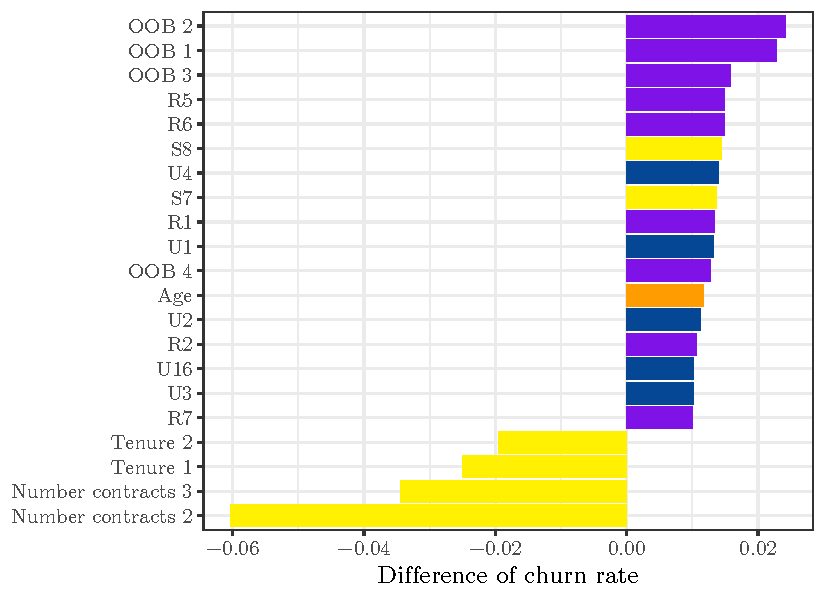
\includegraphics[width=0.9\linewidth]{figures/offset_1p.pdf}
    \caption{Difference in the predicted probability of churn when a standard
    deviation is added separately to each variable. Run on the SIM only dataset.
    Only variables inducing a difference having an absolute value greater than
    0.01 are shown.}
    \label{fig:offset_1p}
\end{figure}

\begin{figure}
    \centering
    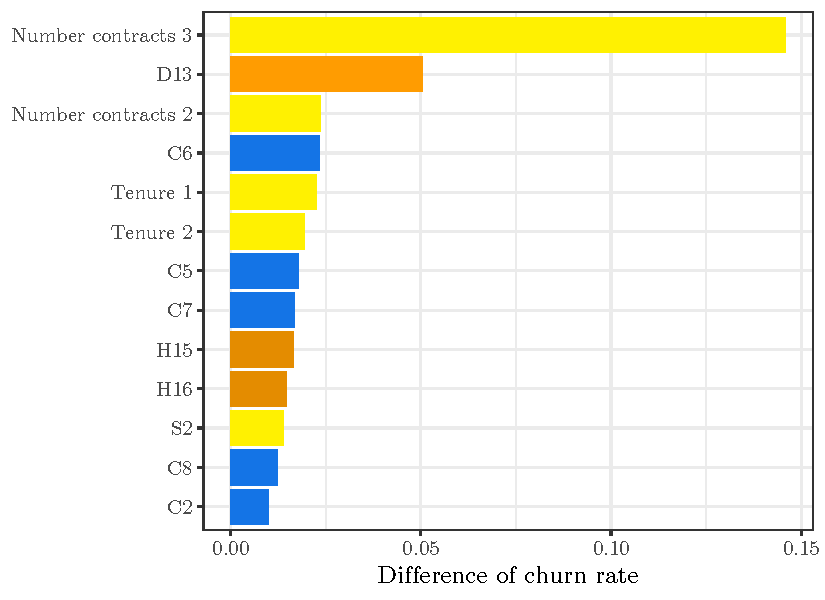
\includegraphics[width=0.9\linewidth]{figures/offset_1m.pdf}
    \caption{Difference in the predicted probability of churn when a standard
    deviation is subtracted separately from each variable. Run on the SIM only
    dataset. Only variables inducing a difference having an absolute value
    greater than 0.005 are shown.}
    \label{fig:offset_1m}
\end{figure}

\section{Comparison to the state of the art}

In this section, we compare our results to other studies in churn prediction. Of
the 20 articles in our bibliography related to churn prediction, 15 are
empirical studies either suggesting a new method or comparing existing methods.
7 of these 15 articles use precision, recall, accuracy, and F-measure as
evaluation measures. These evaluation measures are applicable when the output of
the prediction model is a hard label, such as for a support vector machine or a
decision tree. However, our experiment uses an ensemble model composed of random
forests and the predictions take the form of a score between 0 and 1. This
implies that a decision threshold has to be chosen when classifying customers as
churners or non-churners. The precision, recall, F-measure and accuracy are thus
functions of this threshold, and this does not allow a direct comparison with
these 7 empirical studies. We are left with 8 other studies which use either the
lift at different thresholds (most often 10\%, also named top decile lift), the
expected maximum profit and the area under the ROC curve (AUROC). The results of
these studies are compiled in table \ref{tab:comparison_sota}, along with our
results in the last row.

\begin{table}
    \centering
    \begin{tabular}{llrrr}
        \toprule
        Paper & Best method & AUROC & Lift 10\% & Lift 5\%\\
        \midrule
        \citeauthor*{coussement2017comparative}, \citeyear{coussement2017comparative}
        & Logistic regression & 0.63 & 2.19 & ---  \\
        \citeauthor*{decaigny2018new}, \citeyear{decaigny2018new}
        & Logit Leaf model & 0.87 & 5.34 & ---  \\
        \citeauthor*{oskarsdottir2018time}, \citeyear{oskarsdottir2018time}
        & Similarity forests & 0.87 & 6.05 & ---  \\
        \citeauthor*{zhu2017empirical}, \citeyear{zhu2017empirical}
        & C4.5 with UnderBagging & 0.80 & 4.54 & ---  \\
        \citeauthor*{mitrovic2018operational}, \citeyear{mitrovic2018operational}
        & Random forest & 0.74 & 2.35 & ---  \\
        \citeauthor*{idris2014ensemble}, \citeyear{idris2014ensemble}
        & Ensemble with mRMR & 0.75 & ---  & ---  \\
        \citeauthor*{oskarsdottir2017social}, \citeyear{oskarsdottir2017social}
        & Logistic Regression & 0.89 & ---  & 6.16 \\
        \citeauthor*{verbeke2014social}, \citeyear{verbeke2014social}
        & Relational classifier & ---  & 3.11 & 3.92 \\
        \addlinespace
        Our results & Easy Ensemble & 0.73 & 3.41 & 4.68 \\
        \bottomrule
    \end{tabular}
    \caption{Comparison of our results to other studies in churn prediction.}
    \label{tab:comparison_sota}
\end{table}

We consider our results on the SIM only test set, taking the results of one of
the best performing configurations (no variable selection, no difference or ratio
variables). It is important to notice that the studies mentioned in table
\ref{tab:comparison_sota} obviously do not provide a unique numerical result. In
each of these studies, we considered, whenever possible, the results pertaining
to a dataset similar to ours in terms of churn rate and type of contracts. Also,
when multiple methods are compared in a study, we retained the evaluation
measure of the method performing best. The name of the method retained in each
study is given in the second column of the table.

In terms of area under the ROC curve, we achieve results similar to 2 studies,
both using random forests (the ensemble proposed by \textcite{idris2014ensemble}
contains a random forest, a KNN, and a rotation forest). Also, we perform better
than the logistic regression proposed by \textcite{coussement2017comparative},
but the 4 remaining papers outperform our model by a clear margin. In terms of
lift, we outperform the logistic regression in the first row, the random forest
used in \textcite{mitrovic2018operational} and the combined relational
classifier proposed by \textcite{verbeke2014social}. All other studies yield a
superior lift, both at 5\% and 10\% threshold.

\section{Conclusion}

We summarize here the main findings of our experiments on churn prediction. All
those conclusions are inevitably strongly related to the limited dataset we
considered. We expect that further validation could help in better supporting
such conclusions. Also, the variable selection performed in these experiments
give a useful, restricted scope for the causal analysis in the next chapter by
discarding irrelevant variables.

\begin{itemize}
    \item Feature selection does not reduce performance if at least 30 of the
    most important variables are selected.
    \item Adding difference and ratio variables reduces the performance if no
    feature selection is conducted beforehand.
    \item Due to a lucky domain shift, the trained models actually perform
    better on the test set than on the validation set.
    \item Churn is slightly easier to predict in the loyalty dataset, due to
    the importance of time-related variables.
    \item Important variables include non-exhaustively: the tenure, the
    province, the tariff plan, the number of calls, and the data usage.
    \item The tenure and the number of contracts are associated monotonically to
    the churn probability
    \item Variables related to the amount paid by the customer are associated to
    more churn when they are increased, but the opposite is not true.
\end{itemize}

\chapter{Causal analysis}
\label{ch:caus}

\section{Introduction}
\label{sec:causal_intro}

In this chapter, the application of causal inference to customer data is
explored, in the hope of shedding light on the reasons for customer churn. A
predictive experiment as conducted in the previous chapter indicates which
variables are indicative of a client about to churn, but there is no guarantee
that an intervention on any of these variables will have a positive effect. For
example, the number of contracts registered by a customer has a strong
predictive power as shown in figure
\ref{fig:var_imp_simo_diff_decrease_accuracy}. However, a hypothetical churn
retention action that would sell additional contracts will maybe fail, if
satisfied clients are more prone to buy new contracts but not dissatisfied ones.
In this case, the predictive variable  (number of contracts) and the churn have
a common cause (customer satisfaction). Manipulating the number of contracts
will therefore have no effect on churn. Different tools are needed to discover
true causal relationships between variables. In this chapter, we focus on three
types of models: causal Bayesian networks, information-theoretic filters, and
supervised causal inference. An overview of state-of-the-art methods for each of
these models is given in section \ref{sec:sota_caus}, but we describe them here
in more details.

We begin by introducing \emph{Bayesian networks}, which are graphical models
used to represent probabilistic dependencies between random variables. They are
represented by a \emph{directed acyclic graph} (DAG) where the nodes are random
variables, and a joint probability density is assigned to these variables. We
will use the terms \emph{nodes} and \emph{variable} interchangeably. In a
directed acyclic graph, a node $A$ is a parent of $B$ if there is a direct edge
from $A$ to $B$, $A$ is an ancestor of $B$ if there is a directed path from $A$
to $B$. We can define in a similar way the notions of child, descendant, and
spouse in a directed acyclic graph. Bayesian networks come in a causal variant,
which is defined here \parencite{guyon2007causal}.

\begin{definition}[Causal Bayesian network]

Let $\bm X$ be a set of random variables and $P$ a joint
probability density over $\bm X$. Let $\Gamma$ be a DAG in which the vertices
are $\bm X$. It is required that
\begin{enumerate}[(i)]
    \item for every edge from a node $X\in\bm X$ to a node $Y\in\bm X$, $X$ is a
    direct cause of $Y$, and
    \item for every node $X\in\bm X$, $X$ is probabilistically independent of
    all its non-descendants given its parents, according to $P$:
    \begin{equation}
        X \perp_P (\bm X \setminus \text{Descendents}(X)) | \text{Parents}(X)
    \end{equation}
    where $\text{Descendents}(X)$ is the set of descendent nodes of $X$ and
    $\text{Parents}(X)$ is the set of parent nodes of $X$.
\end{enumerate}
The first condition is required for a Bayesian network to be causal, and the
second condition is called the Markov condition. The tuple $(\bm X, P, \Gamma)$
is a causal Bayesian network iff both conditions are satisfied.

\end{definition}

We denote independence between two variables $X$ and $Y$ according to the
probability density $P$ as $X\perp_P Y$. Similarly, the conditional independence
between two variables $X$ and $Y$ given a set of variables $\bm Z$ is written
$X\perp_P Y|\bm Z$.

The notion of d-separation, as introduced by Pearl (\emph{e.g.} in
\cite{pearl2002causality}), gives a graphical criterion to evaluate the
conditional dependence between two sets of nodes entailed by the Markov
property. This notion uses the terms \emph{chain} (a causal pattern of the form
$X\rightarrow Y\rightarrow Z$), \emph{fork} ($X\leftarrow Y\rightarrow Z$), and
\emph{collider} ($X\rightarrow Y\leftarrow Z$).

\begin{definition}[d-separation]
    Let $X$ and $Y$ be two variables in $\bm X$, and $\Pi$ an undirected path
    between $X$ and $Y$ in the DAG $\Gamma$. The path $\Pi$ is blocked by a set
    of nodes $\bm Z\subset\bm X\setminus\{X, Y\}$ if either of the two following
    statements are true:
    \begin{enumerate}[(i)]
        \item $\Pi$ contains a chain $I\rightarrow Z\rightarrow J$ or a fork
        $I\leftarrow Z\rightarrow J$ such that $Z$ is in $\bm Z$
        \item $\Pi$ does not contain a collider $I\rightarrow Z\leftarrow J$
        such that $Z$ or any of its descendent nodes are in $\bm Z$
    \end{enumerate}
    If all undirected paths $\Pi$ between $X$ and $Y$ are blocked by $\bm Z$,
    then $\bm Z$ d-separates $X$ and $Y$.
\end{definition}

\begin{figure}
    \centering
    \begin{tikzpicture}
        \begin{scope}[every node/.style={ellipse,thick,draw}]
            \node (1) at (0, 0) {Invoice};
            \node (2) at (0, -1.5) {Churn};
            \node (3) at (-3.5, 0) {Data usage};
            \node (4) at (-6.5, 0) {Age};
            \node (5) at (3, 0) {Location};
        \end{scope}
        \begin{scope}[>={Stealth[black]},
            every edge/.style={draw=black,very thick}]
                    \path[->] (1) edge node {} (2);
                    \path[->] (4) edge node {} (3);
                    \path[->] (3) edge node {} (1);
                    \path[->] (5) edge node {} (1);
        \end{scope}
    \end{tikzpicture}
    \caption{An example of causal network illustrating the notion of
    d-separation. Age and invoice are d-separated given data usage, whereas data
    usage and location are no longer d-separated once we know the invoice amount
    or the churn variable.}
    \label{fig:d_sep}
\end{figure}

Using the notion of \emph{d-separation}, we define the conditional independence
between two variables $X$ and $Y$ given $\bm Z$ entailed by a graph $\Gamma$ as
$X\perp_\Gamma Y|\bm Z$. To illustrate this notion, consider the figure
\ref{fig:d_sep}. In this fictional example, the churn is caused solely by the
amount to pay on the invoice. This invoice is in turn determined by the data
usage (and indirectly by the age of the customer), and also by the location: a
customer in a less populated area pays more because establishing the
connectivity is more expensive for the operator. In this configuration, the age
and the invoice are d-separated by the data usage, since knowing the data usage
of a client removes any information the age may bring about the invoice amount.
Also, data usage and location are d-separated given the empty set, since there
is a collider between them. However, if we know the invoice variable, data usage
and location are no longer d-separated, as the knowledge of the invoice allows
to \emph{explain away} one variable with the other. If the client has a large
invoice amount and is living in a populated area, that must mean that its data
usage was probably  high. Note that knowing the churn variable instead of the
invoice would have the same effect, since churn is a direct effect of invoice.

The condition of \emph{faithfulness} is often set onto a causal Bayesian
network:

\begin{definition}[Faithfulness]
\label{def:faith}

A DAG $\Gamma$ is \emph{faithful} to a joint probability density $P$ iff every
dependency entailed by the Markov condition on $\Gamma$ is also
entailed by $P$. That is,

\begin{equation}
\forall X, Y\in\bm X,\forall \bm Z\subset\bm X,\quad
X\not\perp_\Gamma Y|\bm Z\Rightarrow X\not\perp_P Y|\bm Z.
\end{equation}

\end{definition}

Both the Markov conditions and the faithfulness conditions ensure that a given
graph and a given probability density represent accurately the same set of
dependencies and independencies. When both conditions are met, we write
(in)dependence relations without specifying whether it is entailed by $P$ or
$\Gamma$. The faithfulness condition, in particular, ensures that the influence
of a cause onto an effect by multiple causal routes does not cancel itself out.
To demonstrate a violation of this assumption, assume a gene codes both
for the production of a particular protein and for the suppression of another
gene that codes this protein as well. In this case, when the first gene is
removed, the protein is still produced by the other gene, and therefore the
presence of the first gene seems to be independent of the production of the
protein. The probability density $P$ postulates the independence between the two
variables, whereas the causal structure of the problem indicates a causal
link\parencite{hitchcock1997probabilistic}.

Another important concept in Bayesian networks is the notion of \emph{Markov
blanket} of a variable. Informally, this is a set of variables that shields a
given target variable from the influence of the rest of the network. This notion
is useful, for example, in feature selection for machine learning. The Markov
blanket of a target variable is a subset that brings the maximum information
about the target, among all possible sets of variables. Adding any other
variable will bring some information that is already contained in other members,
or in the interaction thereof, of the Markov blanket.

\begin{definition}[Markov blanket]

For a set of random variables $\bm X$, a subset $\bm M\subset\bm X$, and a
variable $Y\in\bm X$, $\bm M$ is the Markov blanket of $Y$ iff for any subset
$\bm V\subset\bm X$, $Y$ is conditionally independent of $\bm V\setminus \bm M$
given $\bm M$.

\end{definition}

In our case, where causal Bayesian networks are represented by a directed
acyclic graph, and where both the Markov and the faithfulness
conditions are met, the Markov blanket of a variable is unique and consists of
its direct causes, its direct effects, and the direct causes of its direct
effects. An example is given in figure \ref{fig:markov_blanket}.

\begin{figure}
    \centering
    \begin{tikzpicture}
        \tikzset{every node/.style={circle, thick},
                >={Stealth[black]},
                every edge/.style={draw=black,very thick}}

        \node[fill=lightorange, draw, minimum size=2.4em] (1) at (0, 0) {$Y$};
        \node[fill=lightblue, draw] (2) at (-1.5, 1.5) {$C_1$};
        \node[fill=lightblue, draw] (3) at (1.5, 1.5) {$C_2$};
        \node[fill=lightblue, draw] (4) at (-1.5, -1.5) {$E_1$};
        \node[fill=lightblue, draw] (5) at (1.5, -1.5) {$E_2$};
        \node[fill=lightblue, draw] (6) at (3, 0) {$S_1$};
        \node[draw] (7) at (-3, 3) {$A_1$};
        \node[draw] (8) at (-3, 0) {$D_1$};
        \node[draw] (9) at (3, 3) {$A_2$};
        \node[draw] (10) at (4.5, 1.5) {$Z_1$};

        \path [->] (2) edge node {} (1);
        \path [->] (3) edge node {} (1);
        \path [->] (1) edge node {} (4);
        \path [->] (1) edge node {} (5);
        \path [->] (6) edge node {} (5);
        \path [->] (7) edge node {} (2);
        \path [->] (4) edge node {} (8);
        \path [->] (9) edge node {} (3);
        \path [->] (10) edge node {} (6);

    \end{tikzpicture}
    \caption{A causal Bayesian network, with the Markov blanket of $Y$
    highlighted in blue.}
    \label{fig:markov_blanket}
\end{figure}

These definitions lay the theoretical background for graphical causal models,
but methods for inference from observational data still need to be derived. The
methods used in this experiment are described in section
\ref{sec:causal_experiments}. A common requirement of some of these methods is
an accurate test of statistical independence between two variables in $\bm X$.
Many statistical independence tests exist, but in our case, we need an estimator
that is able to handle a mix of categorical and continuous variables. We use the
\emph{mutual information}, which is an information-theoretic measure of
statistical dependency. It is more general than the Pearson or the Spearman
correlation coefficient, as it encompasses any type of dependency, and not only
linear or monotonic relationships. Also, it is defined for any two random
variables, regardless of their type or domain. In the case of two discrete
variables $X$ and $Y$ taking values respectively in $\mathcal X$ and $\mathcal
Y$, with a joint probability distribution $P(X, Y)$ and marginal probability
distributions $P(X)$ and $P(Y)$, the mutual information between $X$ and  $Y$ is
defined as \parencite{cover2012elements}

\begin{align}
    I(X, Y) &= \sum_{x\in\mathcal X}\sum_{y\in\mathcal Y}
    P(x, y) \log\left(\frac{P(x, y)}{P(x)P(y)}\right)\label{eq:mi_discrete}\\
    &= H(X) - H(X|Y)\\
    &= H(Y) - H(Y|X)\\
    &=H(X) + H(Y) - H(X, Y)
\end{align}

where $H(X)$ is the entropy of $X$ and $H(X|Y)$ is the conditional entropy of
$X$ given $Y$\parencite{shannon1948mathematical}. The two last equalities
indicate that the mutual information is a symmetric, positive quantity, and
that it can be viewed as the reduction in uncertainty that a variable brings
about the other. A schematic view of these formulae is given in figure
\ref{fig:mi_schematic}. In the case of two continuous variables, an analogous
definition exist \parencite{kolmogorov1956shannon}

\begin{figure}
    \centering
    \begin{tikzpicture}
        \fill[lightblue, opacity = 0.5] (-1,0) circle (1.8);
        \fill[lightorange, opacity = 0.5] (1,0) circle (1.8);
        \draw (-1,0) circle (1.8) node [left] {$H(X|Y)$};
        \draw (1,0) circle (1.8) node [right] {$H(Y|X)$};
        \node at (0,0) {$I(X, Y)$};
        \node at (-3.5,0) {$H(X)$};
        \node at (3.5,0) {$H(Y)$};
        \node at (0,2.2) {$H(X, Y)$};
    \end{tikzpicture}
    \caption{Schematic representation of the relationship between entropy,
    conditional entropy, joint entropy, and mutual information of two discrete
    random variables. The blue circle represents $H(X)$ and the orange circle
    represents $H(Y)$.}
    \label{fig:mi_schematic}
\end{figure}

\begin{align}
    I(X, Y) &= \int_\mathcal X\int_\mathcal Y
    P(x, y) \log\left(\frac{P(x, y)}{P(x)P(y)}\right)dx\,dy\\
    &= h(X) - h(X|Y)\\
    &= h(Y) - h(Y|X)\\
    &= h(X) + h(Y) - h(X, Y)
\end{align}

where $h(X)$ is the differential entropy of $X$ and $h(X|Y)$ is the conditional
differential entropy of $X$ given $Y$. In the case of two normally distributed
variables, we have

\begin{equation}
    \label{eq:mi_gaussian}
    I(X,Y)=-\frac{1}{2}\log(1-\rho^2)
\end{equation}

where $\rho$ is the Pearson correlation coefficient between $X$ and $Y$. Even
though the assumption of normal distribution does not hold in general, empirical
results show that it is still a decent estimator for non-linear dependencies
\parencite{olsen2008impact}. Finally, the mutual information between a continuous
variable $X$ and a discrete variable $Y$ taking values in a finite set $\mathcal
Y$ can be computed as

\begin{equation}
I(X, Y)=h(X) - h(X|Y)=h(X)-\sum_{y\in\mathcal Y}h(X|Y=y)P(Y=y)\label{eq:mi_mixed}
\end{equation}

which means that the mutual information in the mixed case can be computed with
an estimator of the differential entropy of a continuous variable. Following the
discretization method described in \parencite{olsen2008impact}, let $N$ be the
number of values sampled independently and identically from $X$. We divide the
domain $\mathcal X$ of $X$ into $k$ bins of equal size $\Delta$, and we write
$\text{nb}(i)$ the number of samples present in the $i$th bin, $\forall
i\in\{1,\dots,k\}$. The differential entropy of $X$ is estimated with the
\emph{Miller-Madow estimator}

\begin{equation}
    \label{eq:mle_ent}
    \hat h(X) = \sum_{i=1}^k
    \frac{\text{nb}(i)}{N}\log\left(\frac{\text{nb}(i)}{N}\right) + \log\Delta +
    \frac{k-1}{2N}
\end{equation}

It follows that we can compute the mutual information in all possible
configurations of variable types:
\begin{enumerate}[(i)]
    \item Between two discrete variables, using equation \ref{eq:mi_discrete}
    \item Between a continuous variable $X$ and a discrete variable $Y$ with
    equation \ref{eq:mi_mixed} and the differential entropy estimator of
    equation \ref{eq:mle_ent}
    \item Between two continuous variables assuming normal distributions with
    equation \ref{eq:mi_gaussian}
\end{enumerate}

The mutual information can be generalized for any $n$ variables, and is then
named $n$-way \emph{interaction} or \emph{co-information}
\parencite{bell2003co}. A general formula exists, but we are only interested in
the case $n=3$ since it is connected with causal configurations composed of
three variables. All causal configurations of three variables can be easily
enumerated, allowing to develop causal discovery algorithms based solely on the
3-way interaction. In this case, the 3-way interaction (that we simply name
interaction) between three random variables $X_1$, $X_2$, and $Y$ is defined in
\parencite{mcgill1954multivariate} as

\begin{equation}
    \label{eq:int_cond}
    I(X_1, X_2, Y) = I(X_1, X_2) - I(X_1, X_2 | Y)
\end{equation}

where, in the case of a discrete $Y$ taking values in a finite set $\mathcal
Y$, $I(X_1, X_2 | Y)$ can be computed as

\begin{equation}
    \label{eq:int_cond_sum}
    I(X_1, X_2 | Y) = \sum_{y\in\mathcal Y}P(Y=y)I(X_1, X_2 | Y = y)
\end{equation}

A more general definition of conditional mutual information is given in
\parencite{cover2012elements}. But since we consider a classification problem
with $\mathcal Y = \{0, 1\}$, this restricted definition is sufficient for our
purposes.

\section{Scope}

In this chapter, the same dataset as in the predictive modeling chapter is used.
We restrict ourselves to SIM only contracts since it is supposed that the causes
of churn are at least partially different between loyalty and SIM only
contracts. All 5 months of data are used. In order to decrease computation time,
only the first 30 variables in the ranking of the random forest trained in
chapter \ref{ch:churn} are used. Depending on the algorithm being used, a random
subsampling has been applied, also to reach decent computation times. In all
cases, the positive class (churners) is untouched, and a random subset of the
negative class is sampled so that the class ratio is even.

\section{Prior knowledge of churn}
\label{sec:causal_prior}

Bayesian reasoning indicates that we should always take into account our prior
knowledge on a problem when considering the outcome of an experiment designed to
test some hypotheses on this problem. An unlikely theory according to our priors
needs strong evidence to be proven true. Ideally, we should assign a probability
(in the Bayesian sense, that is, a degree of belief) to every theory, and
calculate the probability of the experiment results according to each theory. We
will obviously not conduct this procedure formally in the context of this study,
but the Bayesian methodology is nonetheless useful to keep in mind when
interpreting the results of the causal inference experiments. This section
describes the prior knowledge we have on the causes of churn. It is the result
of discussions and interviews with the data science and business intelligence
teams at Orange Belgium. This prior knowledge is highly valuable since it
incorporates years of experience in churn prevention and customer relationship
in general. We summarize the main causes of churn in four different settings.

\paragraph{Bill shock} This setting has been already evoked multiple times in
chapter \ref{ch:churn}. It occurs when a customer has an unusually large
service usage, which results in an important ``out of bundle'' amount (i.e. the
client is charged much more than usual). This triggers a reaction from the
customer inducing an increased risk of churn. This scenario is well understood
and verified in practice. It is believed to be the most important cause of
churn.

\paragraph{Customer dissatisfaction} Multiple factors influence customer
satisfaction, including quality of service and network quality. A
customer having numerous cuts of network connection during phone calls, or
unable to use properly Orange online services, will be more likely to seek
better alternatives elsewhere.

\paragraph{Wrong positioning} Each customer has different service usage habits.
Some people make a few minutes of phone calls per month, whereas this can be
counted in hours for others. This is why multiple tariff plans are proposed by
the service provider. However, choosing the right tariff plan is sometimes
difficult. On the one hand, if not enough call time is provisioned, an ``out of
bundle'' amount is likely to be charged at the end of the month. On the other
hand, an expensive tariff plan results in a high fixed cost for the customer.
When the needs of a customer does not correspond to the chosen tariff plan, we
say that the customer is wrongly positioned. A wrong positioning results in most
cases to a higher bill that expected, and is a significant cause of churn.

\paragraph{Churn due to a move} It is common to choose a product bundle from a
telecommunication company comprising a subscription for mobile phone, landline
phone, television, and internet connection. In this case, the subscription is
tied to the particular place of domicile of the customer. When the client moves
to another place, it is quite common to also change for another
telecommunication service provider. Therefore, this is a significant cause of
churn, albeit of a different nature from the other settings exposed above.


\paragraph{} These different settings are described informally, and their
translation to the formal definitions of causality presented in section
\ref{sec:causal_intro} is not straightforward. This touches upon philosophical
debates on the definition of causality, which are well beyond the scope of this
thesis. More practically, we wish to find a mapping between the events believed
to be causes of churn and specific instantiations of measurable random
variables. In the case of the first setting, we can reasonably assume that
variables measuring the ``out of bundle'' amount of the customer is a faithful proxy
for bill shock.  Similarly, customer satisfaction can be estimated using,
for example, the number of network cuts during phone calls, or the number of
calls to the customer service. The wrong positioning can also be numerically
estimated, given the tariff plan of the client and its average service usage.
The last setting, churn due to a move, is much more difficult to estimate, as it
is not directly related to the interaction between the client and the
telecommunication services.

In the dataset available for this study, the only measured variables that
translate to potential causes of churn are the ``out of bundle'', the tariff plan
and service usage (phone calls, messages, mobile data). We have no measure
for network quality, customer satisfaction, or propensity to move in the near
future. Also, the wrong positioning is not explicitly encoded and has to be
inferred by the causal inference model from the average service usage and the
current tariff plan.

\section{Experiments}
\label{sec:causal_experiments}

The overall scheme of this experiment consists of running several causal
inference techniques, which give different types of results in various forms,
and extract a general consensus, if any, in the light of the different
assumptions each model put on the data. Indeed, all causal inference methods are
based on different assumptions, and the ability of a given method to infer
causal patterns from observational data lies upon these assumptions.

More specifically, we use 5 different causal inference algorithms:
\noprelistbreak
\begin{itemize}
    \item PC
	\item Grow-shrink (GS)
	\item Incremental Association Markov Blanket (IAMB)
	\item Minimum interaction maximum relevance (mIMR)
	\item D2C
\end{itemize}

For the first three methods, we use the R package \emph{bnlearn}
\parencite{scutari2009learning} for independence tests using mutual information
and asymptotic $\chi^2$ test \parencite{good2013permutation}. For mIMR and D2C,
we use the R package \emph{D2C} \parencite{bontempi2015dependency}, along with
another implementation of mIMR using the mutual information estimator given in
section \ref{sec:causal_intro}. The sample size used in the experiment is given
after the description of each algorithm. In all cases, a false positive rate of
0.05 is chosen for statistical tests of independence.

\subsection{PC}

\paragraph{Description} The PC algorithm \parencite{spirtes1991algorithm}
returns the set of directed acyclic graphs that are faithful to a given
probability distribution. It is based on independence tests between two
variables, conditioned on a set of other variables. It uses the notion of
d-separation to eliminate or find the direction of putative causal links. The PC
algorithm is given in algorithm \ref{alg:pc}, where $\textbf{Adjacencies}(X)$ is
the set of nodes that are adjacent to $X$ in the current version of the result
$\Gamma$. Therefore, it evolves as $\Gamma$ is modified in the algorithm. When
two directions for a causal link are faithful, $\Gamma$ contains an undirected
edge to represent the two directions at once. The result is thus a graph having
directed and undirected edges, but which represent an equivalence class of
undirected acyclic graphs. The idea underlying PC is to A) start with a full
graph, B) remove edges using independence tests with conditioning sets of
increasing size, C) orient colliders using the d-separation property, and D)
find remaining orientations using two more rules. The assumptions underlying
this algorithm are

\begin{enumerate}[(i)]
    \item There is no unmeasured confounder
    \item The statistical tests are correct
    \item The causal relationships between variables are the same for all samples
    \item There exists a DAG $\Gamma$ representing the causal structure that is
    faithful to the underlying joint probability density $P$ (definition
    \ref{def:faith})
\end{enumerate}

If these assumptions hold, then the result of the algorithm is a set of DAGs
that are all faithful to the density probability $P$. The assumption (iii) is
reasonable in our case, but the three others less so.

\begin{algorithm}
    \caption{The PC algorithm}
    \label{alg:pc}
    \begin{algorithmic}
        \State A) Let $\Gamma$ be a complete undirected graph on the set of
        vertices $\bm X$.

        \State B) $n\gets 0$
        \Repeat
            \Repeat
                \State Select a pair of vertices $X$ and $Y$ such that
                \State $\quad\bullet\;X$ and $Y$ are adjacent
                \State $\quad\bullet\;$ there exists a set $\bm
                Z\subseteq\textbf{Adjacencies}(X)\setminus \{Y\}$ that has $n$
                elements
                \State $\quad\bullet\;$ $X\perp Y|\bm Z$.
                \State Remove the edge $X \text{---} Y$ from $\Gamma$
                \State Add $\bm Z$ to $\textbf{Sepset}(X, Y)$ and to $\textbf{Sepset}(Y, X)$
            \Until {no $X$, $Y$ pairs satisfying above conditions can be found}
            \State $n\gets n+1$
        \Until {for each pair $X$ and $Y$, $|\textbf{Adjacencies}(X)\setminus \{Y\}|<n$}

        \State C) For all triplets $X \text{---} Y \text{---} Z$ where there is
        no edge between $X$ and $Z$, orient it as $X\rightarrow Y \leftarrow Z$
        if $Y$ is not in $\textbf{Sepset}(X, Z)$

        \State D)
        \Repeat
            \State Orient all $X\rightarrow Y\text{---} Z$ as $X\rightarrow Y
            \rightarrow Z$
            \State Orient all $X\text{---}Y$ as $X\rightarrow Y$ if there is
            a directed path from $X$ to $Y$
        \Until{no more edges can be oriented}
    \end{algorithmic}
\end{algorithm}

\paragraph{Experimental setting} The PC algorithm is slow when the number of
samples is large since the whole Bayesian network is inferred. Therefore, we
restrict the dataset to 10,000 samples. The implementation given in the package
\emph{bnlearn} is used. The results are given under the form of a directed
acyclic graph.

\subsection{Grow-Shrink}

\paragraph{Description} The GS algorithm \parencite{margaritis2000bayesian} is a
Markov Blanket discovery algorithm efficient even for a large number of
variables. It is based on an estimator that returns a numerical value for the
statistical dependency between two variables, potentially conditioned on a set
of other variables. In our case, we use the mutual information. Consider a
target variable $Y$ and a set of predictor variables $\bm X$. The GS algorithm
constructs the Markov blanket of $Y$, denoted $\MB(Y)$, in three phases
performed in sequence:

\begin{enumerate}[A)]
    \item All variables $X\in\bm X$ are ordered in decreasing order according to
    $I(X, Y)$
    \item Each variable $X\in\bm X$ is added to $\MB(Y)$ iff it is
    conditionally dependent on $Y$, given $\MB(Y)$. That is, iff $I(X,
    Y|\MB(Y)) > 0$.
    \item Each variable $X\in\MB(Y)$ is removed from $\MB(Y)$
    iff it is conditionally independent of the rest of $\MB(Y)$. That
    is, iff $I(X, Y|\MB(Y)\setminus\{X\}) = 0$.
\end{enumerate}

The phase A) is a heuristic to speed up the search, however
\textcite{tsamardinos2003algorithms} pointed out that this delays the inclusion
of spouses, since those have small unconditional relevance to $Y$. Therefore,
more false positives are included before spouses get into $\MB(Y)$.

\paragraph{Experimental setting} The entire set of positive samples is used,
along with a subset of the same size of negative samples. The resulting number
of samples cannot be disclosed due to confidentiality reasons, as it would allow
inferring the actual churn rate in the dataset. The GS algorithm has been
implemented using the independence test in the package \emph{bnlearn}. The
results are given as a list of members of the Markov blanket.


\subsection{Incremental Association Markov Blanket}

\paragraph{Description} The IAMB algorithm \parencite{tsamardinos2003algorithms}
is essentially similar to the GS algorithm, but does not include the sorting
heuristic as a first phase:

\begin{enumerate}[A)]
    \item The variable $X\in\bm X$ maximizing $I(X, Y|\MB(Y))$ is added
    to $\MB(Y)$, repeatedly until all remaining variables are
    independent of $Y$ given $\MB(Y)$.
    \item Each variable $X\in\MB(Y)$ is removed from $\MB(Y)$
    iff it is conditionally independent of the rest of $\MB(Y)$. That
    is, iff $I(X, Y|\MB(Y)\setminus\{X\}) = 0$.
\end{enumerate}

\paragraph{Experimental setting} The experimental setting is the same as for
the GS algorithm.

\subsection{Minimum Interaction Maximum Relevance}

\paragraph{Description} The mIMR filter \parencite{bontempi2010causal} is a
feature selection algorithm that has similarities with the mRMR algorithm
\parencite{peng2005feature}. By using the interaction instead of the redundancy
between the candidate variable and the set of selected variables, causes and
spouses of the target are favored. In order to select only causes, spouses are
eliminated beforehand on the basis of their null unconditional mutual
information with the target. More formally, the main objective of feature
selection is to find a subset $\bm X^*$ of a set of variables $\bm X$ that
maximizes the mutual information with the target $Y$:

\begin{equation}
\bm X^*=\argmax_{\bm X_S\subseteq \bm X} I(\bm X_S,Y)
\end{equation}

Evaluating all possible subsets $\bm X_S$ is computationally infeasible, the
forward selection scheme is therefore adopted. It consists in repetitively
selecting the variable $X_{d+1}^*$ that bring the most improvement given the set
$\bm X_S$ containing the $d$ variables already selected, until a fixed number
$v$ of variables is attained. The improvement is determined in a way that favors
direct causes of $Y$. Consider the interaction equation \ref{eq:int_cond}. The
interaction $I(X_1, X_2, Y)$ can be viewed as the reduction in statistical
dependency between $X_1$ and $X_2$ brought by the knowledge of $Y$. On the one
hand, a positive interaction occurs in 4 types of causal patterns, shown in
figures \ref{fig:chain}, \subref{fig:common_cause}, \subref{fig:brotherhood} and
\subref{fig:grandparent}. On the other hand, a negative interaction occurs only
in the common effect configuration (figure \ref{fig:common_effect}) and the
spouse configuration (figure \ref{fig:spouse}). Furthermore, one can
differentiate between common effect and spouse configurations by noticing that a
spouse of the target has null unconditional relevance with the target (a spouse
is relevant only when the common effect is known). In practice, a statistical
test is used to restrict the set of considered variables to those having
non-null mutual information with the target, written $\bm X_+$. This leads to
the update criterion of mIMR that is a linear combination of relevance and
interaction:

\begin{equation}
    X_{d+1}^* = \argmax_{X_k\in\bm X_+ \setminus \bm X_S}
    \left[ I(X_k,Y) - I(\bm X_S, X_k, Y)\right].
\end{equation}

\begin{figure}
    \centering
    \begin{subfigure}[b]{0.3\linewidth}
        \begin{tikzpicture}
            \tikzset{every node/.style={circle, thick},
                    >={Stealth[black]},
                    every edge/.style={draw=black,very thick}}
            \node[draw, minimum size=2.4em] (1) at (0, 0) {$Y$};
            \node[draw] (2) at (-1.5, 1.5) {$X_1$};
            \node[draw] (3) at (1.5, 1.5) {$X_2$};
            \path [->] (2) edge node {} (1);
            \path [->] (3) edge node {} (1);
        \end{tikzpicture}
        \caption{Common effect}
        \label{fig:common_effect}
    \end{subfigure}
    ~
    \begin{subfigure}[b]{0.3\linewidth}
        \begin{tikzpicture}
            \tikzset{every node/.style={circle, thick},
                    >={Stealth[black]},
                    every edge/.style={draw=black,very thick}}
            \node[draw] (1) at (0, 0) {$X_1$};
            \node[draw] (2) at (-1.5, 1.5) {$X_2$};
            \node[draw, minimum size=2.4em] (3) at (1.5, 1.5) {$Y$};
            \path [->] (2) edge node {} (1);
            \path [->] (3) edge node {} (1);
        \end{tikzpicture}
        \caption{Spouse}
        \label{fig:spouse}
    \end{subfigure}
    ~
    \begin{subfigure}[b]{0.3\linewidth}
        \begin{tikzpicture}
            \tikzset{every node/.style={circle, thick},
                    >={Stealth[black]},
                    every edge/.style={draw=black,very thick}}
            \node[draw, minimum size=2.4em] (1) at (0, 0) {$Y$};
            \node[draw] (2) at (-2, 0) {$X_1$};
            \node[draw] (3) at (2, 0) {$X_2$};
            \path [->] (2) edge node {} (1);
            \path [->] (1) edge node {} (3);
        \end{tikzpicture}
        \caption{Chain}
        \label{fig:chain}
    \end{subfigure}
    ~
    \begin{subfigure}[b]{0.3\linewidth}
        \begin{tikzpicture}
            \tikzset{every node/.style={circle, thick},
                    >={Stealth[black]},
                    every edge/.style={draw=black,very thick}}
            \node[draw, minimum size=2.4em] (1) at (0, 0) {$Y$};
            \node[draw] (2) at (-1.5, -1.5) {$X_1$};
            \node[draw] (3) at (1.5, -1.5) {$X_2$};
            \path [->] (1) edge node {} (2);
            \path [->] (1) edge node {} (3);
        \end{tikzpicture}
        \caption{Common cause}
        \label{fig:common_cause}
    \end{subfigure}
    ~
    \begin{subfigure}[b]{0.3\linewidth}
        \begin{tikzpicture}
            \tikzset{every node/.style={circle, thick},
                    >={Stealth[black]},
                    every edge/.style={draw=black,very thick}}
            \node[draw] (1) at (0, 0) {$X_1$};
            \node[draw, minimum size=2.4em] (2) at (-1.5, -1.5) {$Y$};
            \node[draw] (3) at (1.5, -1.5) {$X_2$};
            \path [->] (1) edge node {} (2);
            \path [->] (1) edge node {} (3);
        \end{tikzpicture}
        \caption{Brotherhood}
        \label{fig:brotherhood}
    \end{subfigure}
    ~
    \begin{subfigure}[b]{0.3\linewidth}
        \begin{tikzpicture}
            \tikzset{every node/.style={circle, thick},
                    >={Stealth[black]},
                    every edge/.style={draw=black,very thick}}
            \node[draw, minimum size=2.4em] (1) at (0, 0) {$X_1$};
            \node[draw] (2) at (-2, 0) {$X_2$};
            \node[draw, minimum size=2.4em] (3) at (2, 0) {$Y$};
            \path [->] (2) edge node {} (1);
            \path [->] (1) edge node {} (3);
        \end{tikzpicture}
        \caption{Grandparent}
        \label{fig:grandparent}
    \end{subfigure}

    \caption{Possible causal patterns between two variables $X_1$ and $X_2$ and
    a target variable $Y$ having non-null interaction.}
    \label{fig:causal_patterns}
\end{figure}

Using the approximation

\begin{equation}
    I(\bm X_S, X_k, Y) \approx \frac{1}{d}\sum_{X_i\in\bm X_S} I(X_i, X_k, Y),
\end{equation}

the forward step can be written as

\begin{align}
    X_{d+1}^* &= \argmax_{X_k\in\bm X_+ \setminus \bm X_S}
    \left[I(X_k,Y) - \frac{1}{d}\sum_{X_i\in\bm X_S} I(X_i, X_k, Y)\right]\\
    &= \argmax_{X_k\in\bm X_+ \setminus \bm X_S}
    \left[I(X_k,Y) - \frac{1}{d}\sum_{X_i\in\bm X_S}
    \left(I(X_i,X_k)-I(X_i, X_k,|Y)\right)\right]\label{eq:mimr_int}\\
    &= \argmax_{X_k\in\bm X_+ \setminus \bm X_S}
    \left[I(X_k,Y) + \frac{1}{d}\sum_{X_i\in\bm X_S} \sum_{y\in\mathcal Y}
    P(Y = y)\left(I(X_i, X_k,|Y=y)-I(X_i,X_k)\right)\right]\label{eq:mimr_final}
\end{align}

where equation \ref{eq:mimr_int} is derived using equation \ref{eq:int_cond} and
similarly \ref{eq:mimr_final} is derived from \ref{eq:int_cond_sum}. The first two variables are selected as

\begin{equation}
    X_1^*, X_2^* = \argmax_{X_i, X_k\in\bm X_+}I([X_i,X_k],Y).
\end{equation}

The mIMR filter is based on some underlying estimator of mutual information
between two variables, and a statistical test of independence for selecting the
set of unconditionally relevant variables $\bm X_+$.

\paragraph{Experimental setting} In this experiment, two implementations are
used:
\noprelistbreak
\begin{itemize}
    \item One using the mutual information estimator described in section
    \ref{sec:causal_intro} and the test of independence in the package
    \emph{bnlearn}.
    \item One assuming normally-distributed continuous variables, allowing to
    compute the mutual information (with equation \ref{eq:mi_gaussian}) and to
    test for independence using the Pearson correlation coefficient. Discrete
    variables are converted to numerical values using one-hot encoding.
\end{itemize}

The drawback of the first method is that the mutual information estimator is
ad-hoc: it assumes a monotonic relationship between two continuous variables
but uses a histogram-based entropy estimator in the mixed case. This may lead to
inconsistencies in the measure of mutual information. On the other hand, the
second method sets the linear assumption on all variables, even on one-hot
encoded categorical variables. For the first implementation, the dataset is
restricted to 10,000 samples, due to the computational cost of the entropy
estimator. In the second implementation, 100,000 samples are used. The results
are provided as a list of the first 15 selected variables, accompanied with the
gain provided by each variable at each iteration of the algorithm.

\subsection{D2C}

\paragraph{Description} The first three causal inference algorithms used in this
section are solely based on statistical independence tests, and therefore are
unable to differentiate between indistinguishable causal patterns, such as the
two variables configuration or the fully-connected three variables
configuration. Since the probability density $P$ is reduced to a set of
(in)dependence relations, any fully connected graph is faithful to $P$ in these
two cases. Asymmetrical patterns exist however in the structural nature of the
dependencies between two variables and the remaining ones. The D2C algorithm
\parencite{bontempi2015dependency} is based on the asymmetry of descriptors
extracted from the Markov blanket of two causally linked variables. Consider two
random variables $X_1$ and $X_2$ such that $X_1$ is a cause of $X_2$, and their
respective Markov blanket $\MB(X_1)$ and $\MB(X_2)$. This setting is pictured in
figure \ref{fig:d2c_mb}. We consider only one cause, effect and spouse per
Markov blanket for the sake of the presentation, but the principles generalize
obviously to any Markov blanket. Two assumptions are however made: i) the only
path between $X_1\cup\MB(X_1)$ and $X_2\cup\MB(X_2)$ is the edge $X_1\rightarrow
X_2$, and ii) $X_1$ and $X_2$ have no common ancestor with their respective
spouse. Failure to satisfy these conditions is expected to be compensated for by
the predictive model. Even though we cannot distinguish between causes, effects
and spouses among $\MB(X_1)$ and $\MB(X_2)$, we can derive several inequalities
using d-separation. Consider the variables $M_1$ and $M_2$, which are members of
respectively  $\MB(X_1)$ and $\MB(X_2)$, but whose relation to $X_1$ and $X_2$
is unknown (that is, $M_1$ is either $C_1$, $E_1$ or $S_1$). We have

\begin{equation}
\label{eq:d2c_ineq}
\begin{cases}
    I(X_1, M_2 | X_2) > I(X_2, M_1 | X_1)\quad\text{if }M_2 = C_2 \\
    I(X_1, M_2 | X_2) = I(X_2, M_1 | X_1)\quad\text{otherwise,}
\end{cases}
\end{equation}

since the only collider configuration between one of $X_1$ and $X_2$ and a
member of the Markov blanket of the other variable is $X_1\rightarrow
X_2\leftarrow C_1$. By computing a population of descriptors

\begin{align}
    D(1, 2)&=\{I(X_1, M_2 | X_2)|\;\forall M_2\in\MB(X_2)\}\\
    D(2, 1)&=\{I(X_2, M_1 | X_1)|\;\forall M_1\in\MB(X_1),\},
\end{align}

equation \ref{eq:d2c_ineq} indicates that the distribution of $D(1, 2)$ differs
from $D(2, 1)$. Other similar inequalities are used to compute 2 other
population of descriptors. The rank of each $M_1$ in $\MB(X_2)$ is also
computed, along with the rank of each $M_2$ in $\MB(X_1)$. The quartiles of the
population of these various descriptors are computed, along with the
mutual information between $X_1$ and $X_2$, and the mutual information
conditioned on $\MB(X_1)$ or $\MB(X_2)$. All these quantities are then used as
features on a machine learning algorithm, whose task is to predict the
probability of a causal link between $X_1$ and $X_2$. The default implementation
of D2C uses a random forest classifier.

\begin{figure}
    \centering
    \begin{tikzpicture}
        \tikzset{every node/.style={circle, thick},
                >={Stealth[black]},
                every edge/.style={draw=black,very thick}}

        \node[draw, minimum size=2.4em] (1) at (0, 0) {$X_1$};
        \node[fill=lightorange, draw] (2) at (1.5, 1.5) {$C_1$};
        \node[fill=lightorange, draw] (3) at (-1.5, -1.5) {$E_1$};
        \node[fill=lightorange, draw] (4) at (-3, 0) {$S_1$};
        \node[draw] (5) at (3, -3) {$X_2$};
        \node[fill=lightblue, draw] (6) at (4.5, -1.5) {$C_2$};
        \node[fill=lightblue, draw] (7) at (1.5, -4.5) {$E_2$};
        \node[fill=lightblue, draw] (8) at (0, -3) {$S_1$};

        \path [->] (1) edge node {} (3);
        \path [->] (2) edge node {} (1);
        \path [->] (4) edge node {} (3);
        \path [->] (1) edge node {} (5);
        \path [->] (5) edge node {} (7);
        \path [->] (6) edge node {} (5);
        \path [->] (8) edge node {} (7);

    \end{tikzpicture}
    \caption{Two causally linked variables and their Markov blanket.}
    \label{fig:d2c_mb}
\end{figure}

\paragraph{Experimental setting}  The D2C model is trained using randomly
generated DAGs, as described in \parencite{bontempi2015dependency} and
implemented in the R package \emph{D2C}. We use 50 DAGs having each a number of
nodes sampled uniformly between 10 and 20, and each DAG generated 50 to 200 data
samples. The function underlying the edge between two nodes is randomly chosen
to be either linear, quadratic or a sigmoid. A Gaussian additive noise of
standard deviation chosen randomly from 0.2 to 1 is added to each directed edge.
The feature extraction phase uses the lazy learning approach
\parencite{bontempi1999lazy} to estimate mutual information, thus avoiding the
linear assumption. We assume a Markov blanket of 4 variables when constructing
the asymmetrical features. Given the high computational cost of feature
extraction, 2,000 samples are used from the customer dataset. The results are
provided as the predicted probability for each variable to be a cause of churn.

\section{Results}

In this section, the colors of the bars in graphs correspond to the
variables categories presented in section \ref{sec:churn_data}:

\begin{itemize}
    \item[\color{themeyellow}$\blacksquare$] \setulcolor{themeyellow}\ul{Subscription}
    \item[\color{themeblue}$\blacksquare$] \setulcolor{themeblue}\ul{Calls and messages}
    \item[\color{darkerblue}$\blacksquare$] \setulcolor{darkerblue}\ul{Mobile data usage}
    \item[\color{themepurple}$\blacksquare$] \setulcolor{themepurple}\ul{Revenue}
    \item[\color{darkerorange}$\blacksquare$] \setulcolor{darkerorange}\ul{Customer hardware}
    \item[\color{themeorange}$\blacksquare$] \setulcolor{themeorange}\ul{Socio-demographic}
\end{itemize}

\subsection{PC}

The output of the PC algorithm is a dense graph linking most of the variables,
but unfortunately, the churn variable is completely disconnected from the rest
of the graph. Note that it also the case for the province, the tariff plan, and
other variables. All of these variables have been ruled out of the Markov
blanket of the churn variable in this algorithm by conditional independence
tests.

\subsection{Grow-Shrink}

The Markov blanket output by the GS algorithm contains 21 variables:

\begin{itemize}
    \item 4 variables related to voice calls (C5, C6, C7, and C8)
    \item 6 variables related to data usage (U1, U2, U3, U4, U10, and U19)
    \item 4 variables related to messages (C1, C2, C3, C4)
    \item ``out of bundle'' amount
    \item Age
    \item Tenure
    \item Number of contracts
    \item A socio-demographic variable (D13)
    \item A hardware-related variable (H15)
    \item A subscription-related variable (S7)
\end{itemize}

As explained by \textcite{tsamardinos2003algorithms}, the heuristic used in GS
that favors variables having high unconditional relevance to the target
increases the probability of false positive, since spouses of the target are not
included in the beginning. Therefore, indirect causes or effects are included
instead. This is particularly obvious in our case since the 4 variables related
to voice calls are highly correlated, and some of them are known to be causes of
the others. The same applies to the groups of variables related to data usage and
messages.

\subsection{Incremental Association Markov Blanket}

The Markov blanket output by the IAMB algorithm contains 2 variables:
\noprelistbreak
\begin{itemize}
    \item The current tariff plan
    \item The previous tariff plan
\end{itemize}

According to IAMB, the churn is therefore independent of all other variables
when we know the current and the previous tariff plan of the customer. This
result is surprising but is stable for different values of false
positive rates: a p-value of up to 0.2 was considered significant for
independence tests, always giving the same result. It is noticeable that IAMB
returns a Markov blanket comprising only categorical variables, while the GS
algorithm gives only numerical variables. While the conditional independence
tests are identical in the two methods, the different order of tests may have
favored one type of variable over the other.

\subsection{Minimum Interaction Maximum Relevance}

Prior to the results of the mIMR algorithm, we show in figures \ref{fig:I_x_x}
and \ref{fig:I_x_x_inter} the mutual information and the interaction matrices of
the 30 most predictive variables. These values are computed using our estimator
presented in section \ref{sec:causal_intro}. Let $X_i$ and $X_j$ be two
variables in our dataset, and let $Y$ be the churn variable. Figure
\ref{fig:I_x_x} shows the mutual information $I(X_i, X_j)$ in the cell of
position $(i, j)$. A line is also added for the churn variable. On the one hand,
one can see that no single variable seems to have a high mutual information with
the churn. This could explain why the PC and IAMB algorithms fail to find a
satisfactory Markov blanket for the churn variable. On the other hand, 3
clusters of high mutual information can clearly be noticed, corresponding to the
summary of voice calls, data usage and messages over the last 3 months. Given
that these variables do not vary randomly from month to month, it is expected
that they are strongly informative about each other, and even more about the
average of the 3 months.

The matrix in figure \ref{fig:I_x_x_inter} shows at position $(i, j)$ the
interaction between two variables $X_i$ and $X_j$ and the churn variable $Y$,
that is, $I(X_i, X_j, Y)$. The row corresponding to the churn is not relevant in
this figure. Recall that the interaction between two variables and a target is
the reduction in statistical dependence that the knowledge of the target brings:

\begin{equation*}
    I(X_1, X_2, Y) = I(X_1, X_2) - I(X_1, X_2 | Y).
\end{equation*}

It is also the amount of mutual dependence to the target that cannot be explained
by bivariate interactions:

\begin{equation*}
    I(X_1, X_2, Y) = I(X_1, Y) + I(X_2, Y) - I([X_1, X_2], Y)
\end{equation*}

We thus seek couples of variables having a negative mutual information with the
churn, since that means that those variables are complementary. Complementary
variables are more likely to either be in a common effect or spouse
configuration (figures \ref{fig:common_effect} and \subref{fig:spouse}) with the
churn. One couple stands out clearly in figure \ref{fig:I_x_x_inter}, the tenure
and the province. The province negatively interacts with most other variables,
meaning that it brings information about the churn only when considering it
conjointly with other variables. The clusters of strongly correlated variables
in figure \ref{fig:I_x_x} have a near-zero interaction since the knowledge of
the churn does not change their distributions.

\begin{figure}
    \centering
    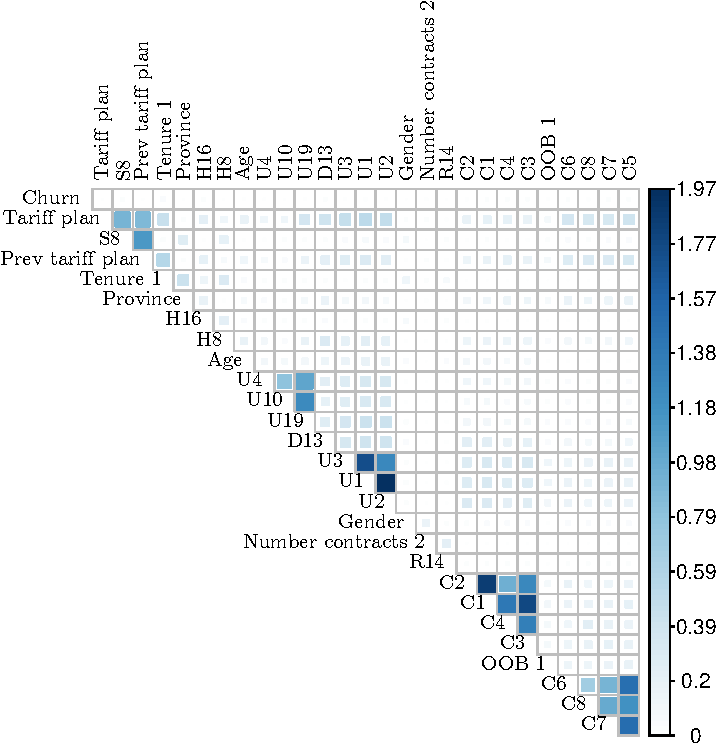
\includegraphics[width=0.8\linewidth]{figures/I_x_x.pdf}
    \caption{Mutual information matrix. The color of the cell indicates the
    statistical dependency between the row and column variables. Clusters of
    high mutual information can be observed for calls, data usage, and messages
    variables. The churn variable has a very low mutual information with other
    variables.}
    \label{fig:I_x_x}
\end{figure}

\begin{figure}
    \centering
    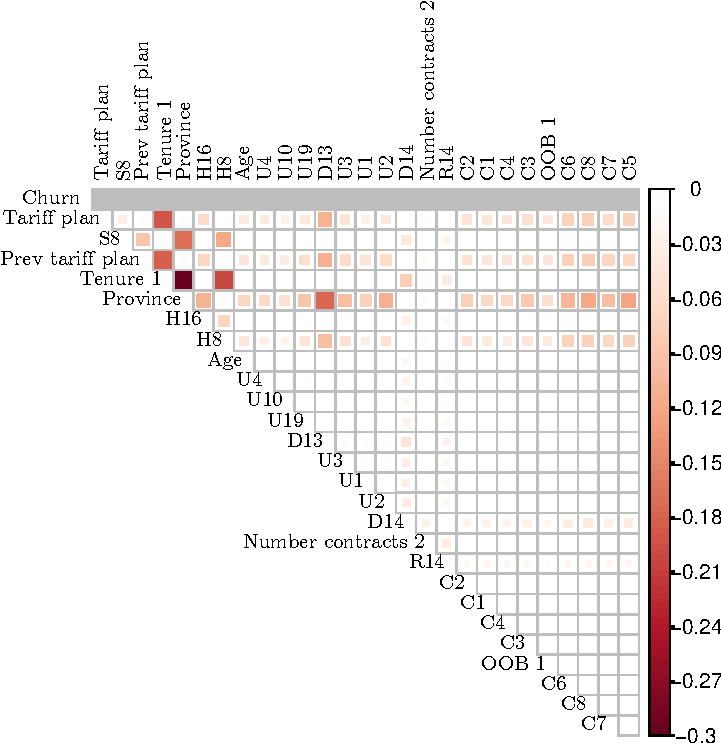
\includegraphics[width=0.8\linewidth]{figures/I_x_x_inter.pdf}
    \caption{Matrix of interaction with the churn. A large negative value
    indicates that the row and column variables bring more information on churn
    when considered together than when considered separately. The  province
    variable has high interaction with most other variables, as well as the
    tariff plan to a lesser extent.}
    \label{fig:I_x_x_inter}
\end{figure}

Figures \ref{fig:mimr_perso} and \ref{fig:mimr_original} show the sequence of
variables selected by the mIMR algorithm, for both our mutual information
estimator (figure \ref{fig:mimr_perso}) and the estimator assuming Gaussian
distributions (figure \ref{fig:mimr_original}). Each row corresponds to one
iteration of the algorithm. The width of the bar corresponds to the value of the
mIMR criterion at this step of the algorithm, that is, the approximated value of
$I(X_k, Y) - I(\bm X_S, X_k, Y)$ where $Y$ is the churn variable, $X_k$ is the
variable under consideration and $\bm X_S$ is the set of variables selected
before $X_k$ (i.e. above $X_k$ on the plot). The two first variables have no
gain since they are directly selected as the pair of variables having the
highest interaction with the target. Unsurprisingly, the first two variables in
figure \ref{fig:mimr_perso} are the tenure and the province (this couple of
variable has the highest negative interaction in figure \ref{fig:I_x_x_inter}).
Background knowledge, as well as figure \ref{fig:I_x_x}, indicate that the
following selected variables are not redundant with one another, up to the 9th
and 10th rows. At these rows, the two variables are both related to the data
usage. That probably indicates that the relevance term $I(X_k, Y)$ is prevailing
over the interaction term $I(\bm X_S, X_k, Y)$.

The selected variables in figure \ref{fig:mimr_original} are mostly similar to
those in \ref{fig:mimr_perso}, except that all categorical variables are not in
the first ranks. Since those are converted to as many numerical variables as
there are categorical levels, the information is spread across multiple
variables. Moreover, each of these new variables is considered to be Gaussian
distributed, therefore not allowing to estimate optimally the mutual
information. Another important difference between \ref{fig:mimr_perso} and
\ref{fig:mimr_original} is that the age and number of contracts are prevalent in
the latter. The importance of age is most probably due to the Gaussian
assumption, which is verified in this case, allowing efficient estimation of its
mutual information with other variables.

\begin{figure}
    \centering
    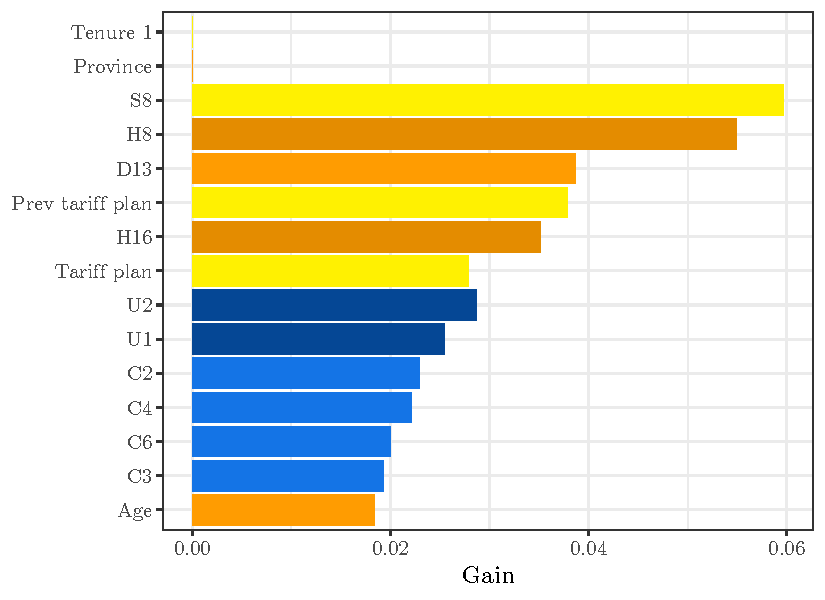
\includegraphics[width=0.9\linewidth]{figures/mimr_perso.pdf}
    \caption{Ranking of variables selected by mIMR with their respective gains,
    using the mutual information estimator of section \ref{sec:causal_intro}.
    There is no gain for the first two variables.}
    \label{fig:mimr_perso}
\end{figure}

\begin{figure}
    \centering
    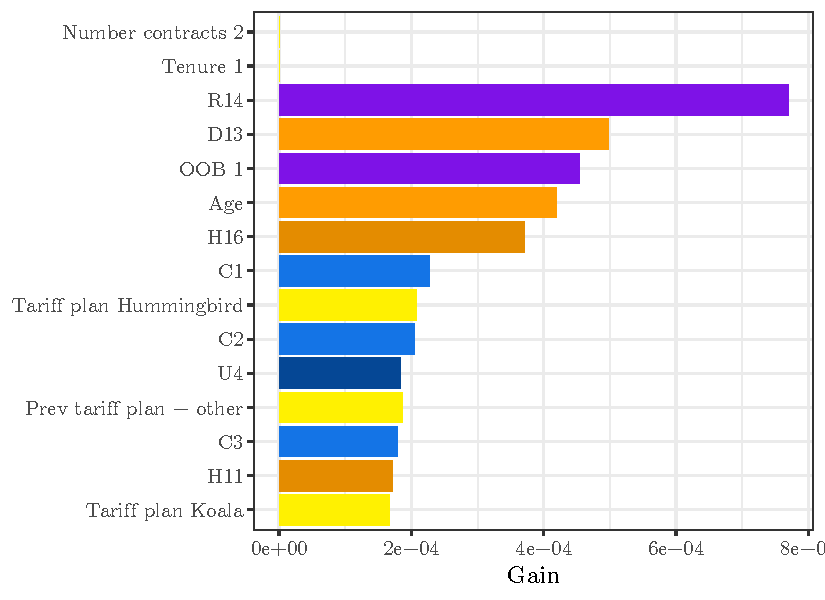
\includegraphics[width=0.9\linewidth]{figures/mimr_original.pdf}
    \caption{Ranking of variables selected by mIMR with their respective gains,
    using one-hot encoding for categorical variables and assuming Gaussian
    distributions. There is no gain for the first two variables.}
    \label{fig:mimr_original}
\end{figure}

\subsection{D2C}

The results from the D2C algorithm are shown in figure \ref{fig:d2c_proba}. To
each variable correspond a probability of being a cause of churn predicted by
the trained random forest. Since the implementation we use for D2C is designed
for numerical variables, one-hot encoding is used. All the variables present in
this plot are related to the tariff plan, previous tariff plan, province of
residence and hardware-related variables. This is consistent with results of
mIMR in figure \ref{fig:mimr_perso}, except for the second and last rows,
related to a categorical socio-demographic variable. Mobile data usage variables
are also present and are the only variables related to service usage in this
graph.

We do not believe that the socio-demographic variables D15 and D16 have a causal
relationship with churn, and this rank is most probably due to an artifact in
the encoding of variables. Indeed, in the data preparation process, we noticed
that data entries labeled as churners tend to have more often missing values in
categorical variables. This issue was caused by the inclusion in the dataset of
customers that already churned, even though some variables have no longer a valid
value for these customers. The solution was to remove such entries from the
dataset, but a related, unforeseen problem may have persisted for these
categorical variables.

\begin{figure}
    \centering
    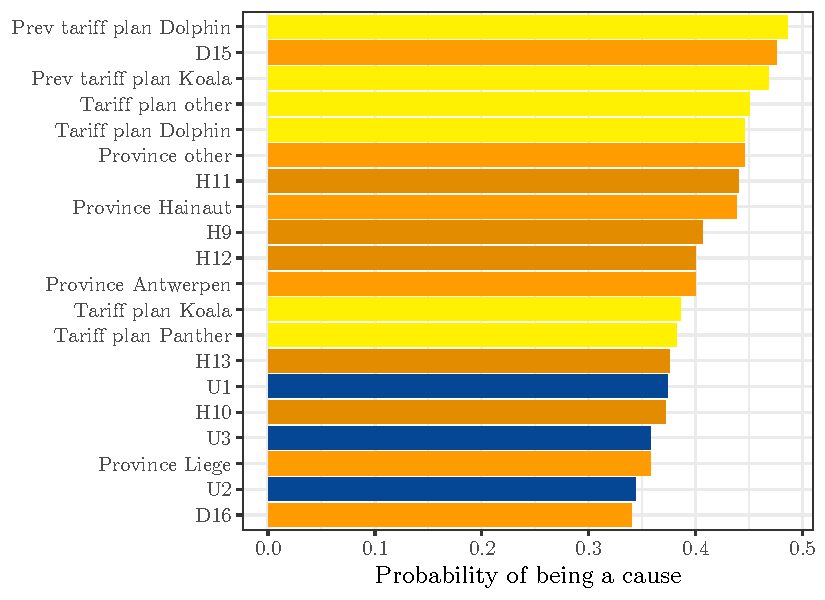
\includegraphics[width=0.9\linewidth]{figures/d2c_proba.pdf}
    \caption{Probability of causal link predicted by D2C}
    \label{fig:d2c_proba}
\end{figure}

\section{Discussion}

The output of the GS and IAMB algorithm correspond to the Markov blanket,
indistinguishably causes, effects and spouses of churn. On the other hand, mIMR
and D2C focus explicitly on direct causes, but a numerical score is provided for
each variable. A choice of threshold has to be made on which variables we
consider to be predicted as causes by these algorithms.

For the mIMR in figure \ref{fig:mimr_perso}, we include all variables up to the
9th and do not consider relevant the following ones. As discussed earlier, the
9th and 10th variables are mostly redundant with one another. Therefore, we can
assume that at this threshold, the relevance term is becoming more important
than the interaction term, and the causal property of the mIMR filter is not
maintained anymore. In the case of mIMR with Gaussian assumption, the threshold
is fixed at the 7th variable, since the following variables show a clear and
distinct decrease in gain.

As for the output of the D2C algorithm, although there seems to be a large
number of variables, most of them are different one-hot encodings of the same
original variable. The most probable causes as predicted by D2C are solely the
tariff plan, previous tariff plan, province of residence, data usage, and a
hardware-related variable (H8). It seems reasonable to consider these 5
variables as predicted causes.

We summarize the results of the 5 algorithms (with the two implementations of
mIMR) in table \ref{tab:causal_summary}. For each variable, we indicate by which
algorithm this variable was output, using the thresholds discussed above. There
is no clear-cut consensus on which variables are causes. It is however
reasonable to consider the number of messages and the duration of voice calls as
\emph{not} being inferred causes of churn, since only the GS algorithm outputs
these variables. On the other hand, the tariff plan and previous tariff plan are
given by all algorithms except for PC, GS, and mIMR with Gaussian assumption. We
do not expect a categorical variable to be correctly predicted as a cause or not
using the Gaussian assumption, the theory that the tariff plan and previous
tariff plan are causes of churn are thus consistent with the observations.

\begin{table}
    \centering
    \begin{tabularx}{\textwidth}{rYYYYYY}
        \toprule
        & PC & GS & IAMB & mIMR 1 & mIMR 2 & D2C \\
        \midrule
        Tenure               & \nok & \ok  & \nok & \ok  & \ok  & \nok \\
        H14                  & \nok & \ok  & \nok & \ok  & \ok  & \nok \\
        D13                  & \nok & \ok  & \nok & \ok  & \ok  & \nok \\
        Data usage           & \nok & \ok  & \nok & \ok  & \nok & \ok  \\
        Tariff plan          & \nok & \nok & \ok  & \ok  & \nok & \ok  \\
        Previous tariff plan & \nok & \nok & \ok  & \ok  & \nok & \ok  \\
        Out of bundle        & \nok & \ok  & \nok & \nok & \ok  & \nok \\
        Nunber of contracts  & \nok & \ok  & \nok & \nok & \ok  & \nok \\
        S7                   & \nok & \ok  & \nok & \ok  & \nok & \nok \\
        H8                   & \nok & \nok & \nok & \ok  & \nok & \ok  \\
        Province             & \nok & \nok & \nok & \ok  & \nok & \ok  \\
        Age                  & \nok & \nok & \nok & \nok & \ok  & \nok \\
        R14                  & \nok & \nok & \nok & \nok & \ok  & \nok \\
        Messages             & \nok & \ok  & \nok & \nok & \nok & \nok \\
        Voice calls          & \nok & \ok  & \nok & \nok & \nok & \nok \\
        \bottomrule
    \end{tabularx}
    \caption{Summary of the results of causal analysis. A green arrow indicates
    which variables are output by each algorithm. The output is the Markov
    blanket for PC, GS and IAMB, and direct causes for mIMR and D2C.}
    \label{tab:causal_summary}
\end{table}

In the absence of a formal procedure to assess these results, we summarize the
results of causal inference from observational data to the following statements:

\begin{itemize}
    \item The  messages, the voice calls, as well as all variables not
    represented in table \ref{tab:causal_summary}, are considered as most
    probably \emph{not inferred causes of churn}.
    \item The tariff plan and previous tariff plan are considered as most
    probably \emph{inferred causes of churn}.
    \item The inferred causal relationship of other variables in the table
    \ref{tab:causal_summary} is undecided.
\end{itemize}

In the light of our prior knowledge on the causes of churn exposed in section
\ref{sec:causal_prior}, we would expect the ``out of bundle'' variable to stand
out more explicitly, but it is only given by mIMR with Gaussian assumption.
However, recall that the distribution of the ``out of bundle'' can roughly be
modeled as the exponential of a Gaussian (see figure \ref{fig:oob}). It is thus
easy to understand why the other inference methods fail to report the causal
link to the churn expected by our priors, due to the different estimators of
mutual information. If it is true that the bill shock is a true cause of churn,
then the results we observe in table \ref{tab:causal_summary} are not
extraordinary. In other words, the credence in this theory is slightly, but not
significantly, undermined.

Two of the other causes of churn according to our prior knowledge are customer
satisfaction and churn due to a move. As explained in section
\ref{sec:causal_prior}, none of the measured variables are direct proxies for
these two putative explanations of churn. The interaction of variables present
in table \ref{tab:causal_summary} might be the most direct display of the
missing causal proxies. This would also explain the presence of variables
seemingly unrelated to our prior knowledge. However, this hypothesis is somewhat
far-fetched and conforming to the faithfulness assumption by engineering
relevant variables would be much more precise and productive. Such missing
variables could be, for example, the number of calls to the customer service, a
measure of the network quality, the number of network cuts during a call, and so
on. Adding these variables would reduce latent confounding if the underlying
causal hypothesis are actually true.

The last of the four expected causes of churn correspond to a wrong positioning
of the customer's tariff plan. This cause is supported by the results in a more
obvious way. The tariff plan and previous tariff plan are reported as causes of
churn by D2C and mIMR, and is also considered part of the Markov blanket by
IAMB. This indicates that the wrong positioning theory is not unlikely. However,
adding a variable that indicates a wrong positioning would be a
stronger, more direct way of verifying this hypothesis.

Given the prior knowledge of churn presented in section \ref{sec:causal_prior},
the mIMR 1 and D2C algorithms seem to better infer relevant variables as direct
causes. Indeed, the bill shock and the wrong positioning imply that the ``out of
bundle'', the tariff plan and the data usage are likely causes of churn. The two
latter are output by mIMR 1 and D2C, whereas mIMR2 outputs the ``out of
bundle''. A model similar to mIMR1 or D2C, but able to correctly handle
variables with an exponential distribution such as the ``out of bundle'', would
be ideal.

Finally, it is important to consider that these results may suffer from sampling
bias. Given that we use a crude random undersampling technique, some causal
patterns in the discarded positive samples may be under-represented in the
resulting training set. This is especially the case for the PC algorithm (using
10,000 samples), the first implementation of mIMR (10,000 samples), and D2C
(2,000 samples). And even though the remaining algorithms use far more samples,
none of them are able to actually take into account the entire set of
non-churners. Furthermore, we have no theoretical guarantee that an even class
ratio is best for inferring causal patterns. Reducing sampling bias in causal
analysis requires the conception of new techniques that are outside the scope of
this thesis.

\chapter{Conclusion}

Lorem ipsum dolor sit amet, consectetur adipiscing elit. Nunc ullamcorper
sollicitudin dolor quisconvallis. Curabitur in dictum sapien. Suspendisse sed
magna sodales, dictum lacus sed, porttitor neque. Duis semper vehicula elit,
quis hendrerit ligula rutrum id. Praesent ac cursus leo, nec scelerisque eros.
Aliquam imperdiet vestibulum turpis, ut hendrerit leo sollicitudin eu. Maecenas
mattis elit quis lectus vestibulum rutrum. Nunc tempus metus sit amet sagittis
porttitor. Integer varius metus aliquet purus pretium, a tincidunt justo
faucibus. Mauris sollicitudin, tortor id tempus suscipit, odio diam dignissim
dolor, quis rutrum libero nisl non nisl. Aliquam felis nisi, mollis nec finibus
a, aliquam eu lectus.

Phasellus in ex hendrerit, malesuada tortor sit amet, sagittis enim. Phasellus
at orci gravida ex malesuada congue ac ac felis. Cras maximus malesuada ligula
id consequat. Praesent bibendum auctor massa eget dignissim. Ut sit amet rhoncus
justo, ut pretium risus. Sed pellentesque nulla eget leo rhoncus malesuada.
Vivamus at diam vitae nibh mattis malesuada non quis turpis. Etiam dignissim
laoreet orci, non sollicitudin sem. Integer non sapien dui. Ut eu elit non
turpis lobortis ullamcorper non a lacus. Integer dictum blandit fringilla.
Quisque tempus metus in dolor rutrum, sed rutrum felis tristique. Nullam ut diam
quis libero imperdiet facilisis. Aenean id nulla quis dolor maximus molestie.
Donec et tortor vel ex hendrerit congue. Nullam pulvinar dui eu sollicitudin
accumsan.

Aliquam nec lectus id leo sagittis feugiat consectetur id diam. Donec sed erat
in turpis vehicula varius. Etiam pharetra dolor dolor. Praesent rhoncus dictum
enim posuere rutrum. Cras et porttitor velit. Fusce condimentum turpis ut eros
aliquet, et finibus dui facilisis. Nullam ullamcorper ex ac tortor dictum
fermentum. Curabitur ultricies diam in consequat fringilla. Mauris a lectus dui.
Mauris in est eget ligula fermentum vestibulum ac a odio. Aliquam erat volutpat.
In ultrices purus id finibus volutpat. Phasellus elementum egestas pellentesque.
Ut porttitor augue sed nunc pellentesque tempus. Vivamus tortor ante, posuere
non magna at, gravida interdum arcu. Maecenas egestas blandit magna, sit amet
tristique enim porta et.

\printbibliography


\end{document}
